% Dies ist die Hauptdatei, von der aus das Gesamtdokument erzeugt wird.  Diese
% Datei sollten Sie zunächst umbenennen, damit sie keinen generischen Namen
% hat!  Dann wird sie mit LuaLaTeX kompiliert.

% In der Datei defs.tex werden alle globalen LaTeX-spezifischen Einstellungen
% vorgenommen
% Jede LaTeX-Datei beginnt mit der Dokumentenklasse.  Für diese Vorlage wurde
% die Klasse "scrreprt" von KOMA-Script gewählt, die in etwa der
% Standardklasse "report" entspricht, allerdings wesentlich mehr Möglichkeiten
% bietet und im gewissen "moderner" ist.  Eine sehr ausführliche Dokumentation
% zu KOMA-Script findet man unter der folgenden Adresse:
% http://mirrors.ctan.org/macros/latex/contrib/koma-script/doc/scrguide.pdf
\documentclass[
  % die Schriftgröße - sollten Sie nicht ändern
  fontsize=12pt,
  % das Papierformat, also DIN A4
  paper=A4,
  % Literaturverzeichnis ins Inhaltsverzeichnis
  bibliography=totoc,
  % andere Verzeichnisse ebenfalls ins Inhaltsverzeichnis
  listof=totoc,
  % abgesetzte Formeln linksbündig
  fleqn,
  % für die Satzspiegelkonstruktion - siehe KOMA-Doku
  DIV=12,
  % Bindekorrektur (linker Rand) - evtl. anpassen
  BCOR=1mm,
  % die im Text verwendeten Sprachen (u.a. für das Paket babel); die
  % letztgenannte (!) Sprache ist die Standardsprache; "n"german steht für die
  % neue Rechtschreibung
  english,ngerman,
  % weil (s.u.) das Paket geometr verwendet wird
  usegeometry,
  % wie Absätze gesetzt werden: ohne Einzug, halbe Zeile Abstand
  parskip=half-
]{scrreprt}

% Beschriftungen für Tabellen kommen linksbündig über die Tabelle
\KOMAoption{captions}{tableheading,nooneline}
\setcaptionalignment[figure]{c}
\setcaptionalignment[table]{l}

% wird für die Titelseite benötigt
\usepackage{geometry}

% Standardpaket für Lokalisation, siehe Option "ngerman" oben
\usepackage{babel}
% Laden von optimierten Trennmustern
\babelprovide[hyphenrules=ngerman-x-latest]{ngerman}

% Standardpaket für mathematische Zusatzfunktionen; wenn Sie keine
% mathematischen Formeln brauchen, können Sie diese Zeile löschen
\usepackage{amsmath}

% die Hauptschrift Libertinus
\usepackage{libertinus-otf}
% die "Schreibmaschinenschrift" Anonymous Pro, angepasst
\usepackage{AnonymousPro}
\setmonofont{AnonymousPro}[Scale=MatchLowercase,FakeStretch=0.85]

% etwas größerer Zeilenabstand als im Buchsatz
\linespread{1.1}

% Paket für Feinkorrekturen an der Typographie, das für ein ausgewogeneres
% Schriftbild sorgt
\usepackage{microtype}

% Paket für kontextsensitive Anführungszeichen
\usepackage{csquotes}
% Shortcut, damit aus dem eigentlich falschen Zeichen " richtige
% Anführungszeichen je nach Sprache werden
\MakeOuterQuote{"}

% Paket, das den Befehl \includegraphics ermöglicht
\usepackage{graphicx}

% komfortablere Aufzählungen als in Standard-LaTeX; ein Beispiel findet man in
% chap3.tex
\usepackage{enumitem}

% Paket für mehr als die üblichen Standardfarben
\usepackage[dvipsnames]{xcolor}
% Definition der "Hausfarben" der HAW
\definecolor{haw}{HTML}{003CA0}
\definecolor{haw2}{HTML}{0096D2}
\definecolor{haw3}{HTML}{A0BEDC}
\definecolor{darkgreen}{rgb}{0, 0.5, 0}
\definecolor{background}{HTML}{EEEEEE}
\definecolor{delim}{RGB}{20,105,176}
\colorlet{punct}{red!60!black}
\colorlet{numb}{magenta!60!black}

% typographisch anspruchsvolle Tabellen; siehe chap3.tex
\usepackage{booktabs}

% zum Erstellen des Literaturverzeichnisses; der gängige Stil APA ist hier
% bereits eingestellt
\usepackage[style=apa]{biblatex}
% eine Beispieldatei für ein Literaturverzeichnis
\addbibresource{bachelorarbeit.bib}

% für die Erzeugung der Grafiken in chap3.tex; wenn Sie PGF/TikZ nicht
% verwenden wollen, können Sie diese Zeilen entfernen
\usepackage{tikz}
% Zusatzbibliotheken für TikZ, die in den genannten Beispielen verwendet
% werden
\usetikzlibrary{calc,intersections,angles,3d}

% für die Erzeugung des Codeblocks in chap3.tex; wenn in Ihrer Arbeit keine
% Codeblöcke vorkommen, können Sie diese Zeilen entfernen
\usepackage{listings}

% see https://tex.stackexchange.com/questions/83085/how-to-improve-listings-display-of-json-files
\lstdefinelanguage{json}{
    basicstyle=\normalfont\ttfamily,
    numbers=left,
    numberstyle=\scriptsize,
    stepnumber=1,
    numbersep=8pt,
    showstringspaces=false,
    breaklines=true,
    frame=lines,
    backgroundcolor=\color{background},
    literate=
    *{0}{{{\color{numb}0}}}{1}
        {1}{{{\color{numb}1}}}{1}
        {2}{{{\color{numb}2}}}{1}
        {3}{{{\color{numb}3}}}{1}
        {4}{{{\color{numb}4}}}{1}
        {5}{{{\color{numb}5}}}{1}
        {6}{{{\color{numb}6}}}{1}
        {7}{{{\color{numb}7}}}{1}
        {8}{{{\color{numb}8}}}{1}
        {9}{{{\color{numb}9}}}{1}
        {:}{{{\color{punct}{:}}}}{1}
        {,}{{{\color{punct}{,}}}}{1}
        {\{}{{{\color{delim}{\{}}}}{1}
        {\}}{{{\color{delim}{\}}}}}{1}
        {[}{{{\color{delim}{[}}}}{1}
        {]}{{{\color{delim}{]}}}}{1},
}
% see https://tex.stackexchange.com/questions/152829/how-can-i-highlight-yaml-code-in-a-pretty-way-with-listings
\newcommand\YAMLcolonstyle{\color{red}\mdseries}
\newcommand\YAMLkeystyle{\color{black}\bfseries}
\newcommand\YAMLvaluestyle{\color{blue}\mdseries}

\makeatletter

\newcommand\language@yaml{yaml}

\expandafter\expandafter\expandafter\lstdefinelanguage
\expandafter{\language@yaml}
{
    keywords={true,false,null,y,n},
    keywordstyle=\color{darkgray}\bfseries,
    basicstyle=\YAMLkeystyle,
    sensitive=false,
    comment=[l]{\#},
    morecomment=[s]{/*}{*/},
    commentstyle=\color{purple}\ttfamily,
    stringstyle=\YAMLvaluestyle\ttfamily,
    moredelim=[l][\color{orange}]{\&},
    moredelim=[l][\color{magenta}]{*},
    moredelim=**[il][\YAMLcolonstyle{:}\YAMLvaluestyle]{:},
    morestring=[b]',
    morestring=[b]",
    literate =    {---}{{\ProcessThreeDashes}}3
        {>}{{\textcolor{red}\textgreater}}1
        {|}{{\textcolor{red}\textbar}}1
        {\ -\ }{{\mdseries\ -\ }}3,
}

\lst@AddToHook{EveryLine}{\ifx\lst@language\language@yaml\YAMLkeystyle\fi}
\makeatother
\newcommand\ProcessThreeDashes{\llap{\color{cyan}\mdseries-{-}-}}

\lstdefinelanguage{math}{
    keywords={SIGNED, UNSIGNED},
    sensitive=true,
    morekeywords={bis},
    keywordstyle=\color{blue}\bfseries,
    comment=[l]\%,
    string=[b]",
    morestring=[b]',
    moredelim=*[s][\color{gray}]{/*}{*/},
    morekeywords={[2]Beispiel},
    keywordstyle={[2]\color{haw2}\bfseries},
}

% Anpassung des Erscheinungsbildes des Codeblocks; mehr dazu in der
% Dokumentation des Pakets "listings"
\lstdefinestyle{mystyle}{
    backgroundcolor=\color{gray!20},
    keywordstyle=\color{haw2},
    numberstyle=\footnotesize\color{haw},
    basicstyle=\ttfamily\small,
    captionpos=t,
    frame=single,
    framerule=0pt,
    keepspaces=true,
    numbers=left,
    numbersep=6pt,
    belowcaptionskip=1em,
    aboveskip=\bigskipamount,
}

\lstdefinestyle{custom_daniel}{
    backgroundcolor=\color{gray!20},
    basicstyle=\ttfamily\small,
    keywordstyle=\color{haw2},
    commentstyle=\color{gray},
    numberstyle=\footnotesize\color{haw},
    stringstyle=\color{darkgreen},
    numbers=left,
    breaklines=true,
    keepspaces=true,
    showspaces=false,
    showstringspaces=false,
}
\lstset{style=mystyle}
% damit es "Codeblock" und nicht "Listing" heißt
\renewcommand{\lstlistingname}{Codeblock}

% für die Verlinkung innerhalb des PDF-Dokuments, für PDF-Lesezeichen und
% PDF-Metadaten; dieses Paket sollte üblicherweise immer als letztes geladen
% werden
\usepackage[colorlinks=true,allcolors=haw,hyperfootnotes=false,pageanchor=true,linktoc=all]{hyperref}

% für die Druckversion können Sie die obige Zeile durch die folgende ersetzen,
% damit Links nicht blau dargestellt werden:
% \usepackage[draft]{hyperref}

% Metadaten des PDF-Dokumentes; setzen Sie hier Ihren eigenen Namen sowie den
% Titel Ihrer Arbeit ein
\hypersetup{pdfauthor={Daniel Freire Mendes}}
\hypersetup{pdftitle={Performance-Optimierung von Datenbanken}}

\usepackage{subcaption}
\usepackage{float}
\usepackage[labelfont=bf]{caption}
% \includeonly{benchmarks}
% BibTex see here: https://github.com/Hannah-Sten/TeXiFy-IDEA/issues/1390
% Wenn das Kommentarzeichen entfernt wird, kann man mit einem Befehl wie
%
% \includeonly{chap2,chap3}
%
% erreichen, dass nur ausgewählte Dateien kompiliert werden.  Das ist für die
% Arbeit an umfangreichen Dokumenten hilfreich, weil es Zeit spart.  Für das
% Erstellen des fertigen Dokuments muss der Befehl natürlich wieder
% auskommentiert werden, damit alle Referenzen aktuell sind und die
% Seitenzahlen stimmen.

% Hier beginnt das eigentliche Dokument.  Sie können weitere Dateien
% hinzufügen und natürlich auch vorhandene weglassen.  Die vorhandene
% Dateistruktur ist lediglich als Beispiel gedacht.
\begin{document}
% In dieser Umgebung wird die Titelseite separat vom restlichen Text gesetzt
\begin{titlepage}
  % andere Seitenränder als im Rest der Arbeit
  \newgeometry{lmargin=2cm,tmargin=7mm,rmargin=5mm,bmargin=1cm}
  % die "Hausfarbe" der HAW; diese und die folgenden Einstellungen sind lokal
  % und gelten nur innerhalb der Umgebung "titlepage"
  \color{haw}
  % Blocksatz für die Titelseite deaktivieren
  \raggedright
  % Logo rechtsbündig setzen
  \hfill
\includegraphics[width=7cm]{PNGs/General/HAW_Marke_RGB_300dpi}\\

  % vertikaler Abstand
  \vspace{5cm}

  % Wahl der "Hausschrift" Open Sans der HAW, die als Schrift auf Ihrem
  % Rechner installiert sein muss
  \setmainfont{Open Sans}
  % etwas kleiner als üblich
  \small
  % fett und in Majuskeln
  \textbf{BACHELORARBEIT}

  % vertikaler Abstand
  \vspace{8mm}

  % der Titel der Arbeit als "Seite in der Seite"; natürlich müssen Sie hier
  % Ihren Titel eintragen
  \begin{minipage}{0.8\linewidth}
    % Wahle der zweiten "Hausschrift" der HAW, die ebenfalls auf Ihrem Rechner
    % bereits vorhanden sein muss
    \setmainfont{Martel Heavy}
    % ziemlich große Schrift
    \LARGE
    % [1mm] steht jeweils für einen etwas größeren Durchschuss
    Performance -\\[1mm]
    Optimierung\\[1mm]
    von Datenbanken\\
    % am Ende noch ein waagerechter Strich, das CD will es so...
    \,\rule{11mm}{1.2mm}
  \end{minipage}

  % vertikaler Abstand, überraschenderweise
  \vspace{1cm}

  % hier korrektes Datum und Ihren Namen eingeben
  % TODO(Daniel): update this
  vorgelegt am 26. März 2022\\
  Daniel Freire Mendes

  % letzter vertikaler Abstand für heute
  \vspace{5cm}

  % noch eine "Seite in der Seite", etwas nach rechts geschoben
  \hspace*{37mm}
  \begin{minipage}{0.5\linewidth}
    % Namen und Titel der beiden Prüfer eintragen
    \begin{tabular}{@{}ll}
      Erstprüferin: & Prof. Dr. Stefan Sarstedt\\[-.3mm]
      Zweitprüfer: & Prof. Dr. Olaf Zukunft \\
    \end{tabular}\\

    % noch ein horizontaler Strich
    \,\rule{9mm}{1mm}\\[1.5mm]

    \textbf{HOCHSCHULE FÜR ANGEWANDTE}\\
    \textbf{WISSENSCHAFTEN HAMBURG}\\
    Department Informatik\\
    Berliner Tor 7\\
    20099 Hamburg
  \end{minipage}
\end{titlepage}
% setzt die Geometrie wieder auf die Standardwerte zurück
\restoregeometry

% für die Seite mit dem Abstract keine Seitenzahl ausgeben
\thispagestyle{empty}
% TODO(Daniel): write text here
\section*{Zusammenfassung}

% Hier ersetzen Sie bitte die vorhandenen Texte durch Ihre eigenen
% Zusammenfassungen
Der Arbeit beginnt mit einer kurzen Beschreibung ihrer zentralen Inhalte, in
der die Thematik und die wesentlichen Resultate skizziert werden.  Diese
Beschreibung muss sowohl in deutscher als auch in englischer Sprache vorliegen
und sollte eine Länge von etwa 150 bis 250 Wörtern haben.  Beide Versionen
zusammen sollten nicht mehr als eine Seite umfassen.  Die Zusammenfassung
dient u.\,a.\ der inhaltlichen Verortung im Bibliothekskatalog.

% Zum Wechseln der Sprache siehe den Kommentar in chap3.tex
{
  \begin{otherlanguage}{english}
    % TODO(Daniel): write text here
    \section*{Abstract}

    The thesis begins with a brief summary of its main contents, outlining the
    subject matter and the essential findings.  This summary must be provided
    in German and in English and should range from 150 to 250 words in length.
    Both versions combined should not comprise more than one page.  Among
    other things, the abstract is used for library classification.
  \end{otherlanguage}
}

% In der Titelei werden römische Ziffern für die Seitenzahlen verwendet;
% gleichzeitig wird durch diesen Befehl die aktuelle Seitenzahl auf eins
% gesetzt
\pagenumbering{Roman}

% Inhaltsverzeichnis
\tableofcontents

% Abbildungsverzeichnis, kann evtl. weggelassen werden
\listoffigures

% Tabellenverzeichnis, kann evtl. weggelassen werden
\listoftables

% weitere Verzeichnisse (z.B. Codeblöcke) sind theoretisch möglich

% neue Seite, vorsichtshalber
\clearpage
% ab jetzt arabische Ziffern und wieder auf eins setzen
\pagenumbering{arabic}
%! Author = danielmendes
%! Date = 21.10.24
\chapter{Überblick}

\section{Einführung in Benchmarks}

Benchmarks dienen dazu, praktisch und effektiv zu untersuchen, wie sich ein
System unter Last verhält. Die wichtigste Erkenntnis, die man aus Benchmarks
gewinnen kann, sind die Probleme und Fehler, die man systematisch dokumentieren
und nach Priorität abarbeiten sollte. Das Ziel von Benchmarks ist die Reduzierung
und Bewertung von unerwünschtem Verhalten sowie die Analyse, wie sich das
System derzeit und unter simulierten, zukünftigen, anspruchsvolleren Bedingungen
verhalten könnte.

Es gibt zwei verschiedene Techniken für Benchmarks. Die erste zielt darauf ab,
die Applikation als Ganzes zu testen (full-stack). Dabei wird nicht nur die
Datenbank getestet, sondern die gesamte Applikation, einschließlich des Webservers,
des Netzwerks und des Applikationscodes. Der Ansatz dahinter ist, dass ein Nutzer
genauso lange auf eine Abfrage warten muss, wie das gesamte System benötigt.
Daher sollte diese Wartezeit so gering wie möglich sein. Es kann dabei vorkommen,
dass MySQL nicht immer das Bottleneck ist.\footnote{Gemeint ist ein Engpass beim Transport von Daten oder Waren, der maßgeblichen Einfluss auf die Abarbeitungsgeschwindigkeit hat. Optimierungsversuche an anderer Stelle führen oft nur zu geringen oder gar keinen messbaren Verbesserungen der Gesamtsituation. (\cite{bottleneck})}

Full-Stack-Benchmarks haben jedoch auch Nachteile. Sie sind schwieriger zu erstellen
und insbesondere schwieriger korrekt einzurichten. Wenn man lediglich verschiedene
Schemas und Abfragen in MySQL auf ihre Performance testen möchte, gibt es sogenannte
Single-Component-Benchmarks. Diese analysieren ein spezifisches Problem in der
Applikation und sind deutlich einfacher zu erstellen. Ein weiterer Vorteil besteht
darin, dass nur ein Teil des gesamten Systems getestet wird, wodurch die Antwortzeiten
kürzer sind und man schneller Ergebnisse erhält.

Wenn bei Benchmarks schlechte Designentscheidungen getroffen werden, kann dies zu einer
falschen Interpretation des Systems führen, da die Ergebnisse nicht die Realität widerspiegeln.
Die Größe des Datensatzes und des Workloads muss realistisch sein. Idealerweise verwendet
man einen Snapshot\footnote{Snapshots bestehen größtenteils aus Metadaten, die den Zustand Ihrer Daten definieren, und sind keine vollständige Duplikation der Daten auf Ihrer Festplatte. Snapshots werden häufig für Test-/Entwicklungsaufgaben verwendet. (\cite{snapshot}) } des tatsächlichen produktiven Datensatzes.
Gibt es keine Produktionsdaten, sollten die Daten und der Workload simuliert werden,
da realistische Benchmarks komplex und zeitaufwendig sein können.

Häufige Fehler beim Durchführen von Benchmarks sind unter anderem, dass nur ein kleiner Teil
der tatsächlichen Datensatzgröße verwendet wird und die Datensätze unkorrekt gleichmäßig
verteilt sind. In der Realität können Hotspots auftreten. Bei zufällig generierten Werten
kommt es hingegen häufig zu unrealistisch gleichmäßig verteilten Datensätzen. Ein weiterer
Fehler besteht darin, dass man beim Testen einer Anwendung nicht das tatsächliche
Benutzerverhalten nachstellt. Wenn gleiche Abfragen in einer Schleife ausgeführt werden,
muss man außerdem auf das Caching achten, da sonst falsche Annahmen über die Performance
getroffen werden können. Zudem wird oft die Warmmachphase des Systems vollständig ignoriert.
Kurze Benchmarks können schnell zu falschen Annahmen über die Performance des Systems führen.

Um verlässliche Ergebnisse zu erhalten, sollte ein Benchmark ausreichend lange laufen,
um den stabilen Zustand des Systems zu beobachten, insbesondere bei Servern mit großen
Datenmengen und viel Speicher. Dabei ist es wichtig, so viele Informationen wie möglich zu
erfassen und sicherzustellen, dass der Benchmark wiederholbar ist, da unzureichende oder
fehlerhafte Tests wertlos sind. Außerdem ist es wichtig, die Ergebnisse in einem Diagramm
darzustellen, da auftretende Phänomene sonst anhand einer tabellarischen Darstellung nicht
erkannt werden können.


\section{Measures}
\begin{itemize}[label={--}]
    \item \textbf{Durchsatz (Throughput):} Der Durchsatz ist die Anzahl an Transaktionen pro Zeiteinheit.
    Er ist standardisiert, und Datenbankanbieter versuchen, diesen zu optimieren.
    Meistens werden Transaktionen pro Sekunde (oder manchmal pro Minute) als Einheit verwendet.
    \item \textbf{Antwortzeiten (Latenz):} Die Antwortzeit misst die gesamte Zeit, die für eine Abfrage benötigt wird.
    Diese kann, abhängig von der Applikation, in Mikrosekunden (µs), Millisekunden (ms), Sekunden oder Minuten angegeben werden.
    Von dieser Zeit können aggregierte Antwortzeiten wie Durchschnitt, Maximum, Minimum und Perzentile abgeleitet werden.
    Das Maximum ist oft eine weniger sinnvolle Metrik, da es sich nicht gut wiederholen lässt.
    Daher nutzt man eher Perzentile bei den Antwortzeiten.
    Wenn beispielsweise das 95. Perzentil der Antwortzeit bei 5 ms liegt, bedeutet dies, dass mit einer Wahrscheinlichkeit von 95 \% die Abfrage in weniger als 5 ms abgeschlossen ist.
    \item \textbf{Nebenläufigkeit (Concurrency):} Die Nebenläufigkeit auf dem Webserver lässt sich nicht zwangsläufig auf den Datenbankserver übertragen.
    Eine genauere Messung der Gleichzeitigkeit auf dem Webserver besteht darin, zu bestimmen, wie viele gleichzeitige Anfragen zu einem bestimmten Zeitpunkt ausgeführt werden.
    Es kann auch geprüft werden, ob der Durchsatz sinkt oder die Antwortzeiten steigen, wenn die Gleichzeitigkeit zunimmt.
    Beispielsweise benötigt eine Website mit „50.000 Benutzern gleichzeitig“ vielleicht nur 10 oder 15 gleichzeitig laufende Abfragen.
    \item \textbf{Skalierbarkeit (Scalability):} Skalierbarkeit ist wichtig für Systeme, die ihre Performance unter unterschiedlich starken Workloads beibehalten müssen.
    Ein ideales System würde doppelt so viele Abfragen beantworten (Throughput), wenn doppelt so viele „Arbeiter“ versuchen, die Aufgaben zu erfüllen.
    Die meisten Systeme sind jedoch nicht linear skalierbar und zeigen Leistungseinbußen, wenn die Parameter variieren.
\end{itemize}


\section{Tools}\label{sec:tools}

\subsection{Einführung}\label{subsec:einfuhrung}

Als Haupttool, um Benchmarktests durchzuführen, habe ich mich für Sysbench \cite{sysbench_repo}
entschieden. Sysbench ist ein Open-Source-Tool, das ein skriptfähiges, multi-threaded Benchmark-Tool
ist, das auf LuaJIT basiert. Es wird auch hauptsächlich für Datenbankbenchmarks verwendet, kann
jedoch auch dazu eingesetzt werden, beliebig komplexe Arbeitslasten zu erstellen, die keinen
Datenbankserver erfordern. Dabei werden Tests auf verschiedenen Systemressourcen, wie CPU, S
peicher, I/O und Datenbanken wie MySQL \cite{sysbench_mysql} verwendet.

Im Zuge der Recherchearbeit habe ich mir auch andere Benchmarking-Tools betrachtet, wie z.B.
Benchbase \cite{DifallahPCC13} oder mybench \cite{mybench_repo}. Die größten Vorteile von
Sysbench habe ich in der Skriptfähigkeit und Flexibilität gesehen. D.h. dass ich benutzerdefinierte
Benchmarks schneller und unkompliziert erstellen kann. Außerdem hat sich Sysbench als de facto
Standard im Bereich der Datenbankbenchmarks etabliert \cite{mybench_comparison}. Dadurch stehen
eine breite Nutzerbasis und viele verfügbare Ressourcen zur Verfügung. Im Vergleich zu den
anderen Tools bietet allerdings Sysbench eine weniger präzise Steuerung der Ergebnisrate
und der Transaktionen. Außerdem haben Tools wie mybench die Möglichkeit, in Echtzeit umfassende
Visualisierungen darzustellen. Damit können Metriken live in einem Diagramm angezeigt werden
\cite{mybench_user_interface}. Dieses Feature ist sicherlich hilfreich, aber in meinem Fall habe
ich abgewogen und bin zu dem Entschluss gekommen, dass die einfachere Bedienung für mich der
ausschlaggebende Grund, neben dem Fakt, dass Sysbench der de facto Standard ist.

Trotzdem kann man nicht komplett auf Graphen verzichten, da beispielweise Entwicklungen
im Laufe einer Zeitmessung in einem Kurvenverlauf deutlich besser zu erkennen sind als in einer CSV-Datei.
Anhand der reinen Zahlen aus diesen Tabellen fallen diese wiederkehrende Trends unter anderem nicht direkt auf.
Die Kennzahlen, die mithilfe von Sysbench ermittelt werden, werden in einer CSV-Datei gespeichert.
Um diese tabellarische Form in eine Grafische umzuwandeln, gibt es unterschiedliche Tools, die widerum
eigene Vor- und Nachteile bieten.

Die erste mögliche Alternative stellt das Tool Gnuplot \cite{gnuplot} dar.
Mit diesem lassen sich CSV-Dateien sehr gut darstellen. Wenn man aber beispielweise nur bestimmte Spalten
aus der Tabelle anzeigen lassen will, dann kommt man schnell an seine Granzen.
Um besser Anpassungsfähig sein zu können, habe ich mich letztlich dazu entschieden ein eigenes Python-Script
zu schreiben, die mithilfe der Libraries pandas (//TODO (Daniel): find source) matplotlib.pyplot (//TODO (Daniel): find source)
die Graphen erstellt.

\subsection{Einführung in die Tools}\label{subsec:einfuhrung-in-die-tools}

Als allererstes muss der MySQL-Server (oder eine anderes relationales Datenbankverwaltungssystem, das von Sysbench
unterstützt wird) lokal auf dem Rechner gestartet sein. Wichtig ist dabei die User -und Passwortdaten zu merken, da
diese von den Sysbench - Benchmarks benötigt werden. Nachdem das RDBMS gestartet worden ist, muss zudem eine
Datenbank erstellt werden. Dies könnte unter anderem so aussehen:

\begin{lstlisting}[label={lst:create database}]
CREATE DATABASE sbtest;
\end{lstlisting}

Nachdem man die Datenbank erstellt hat, muss das Tool Sysbench zunächst installiert werden.
Als nächstes machen wir uns mit dem Tool und den verschiedenen Argumenten,
die beim Aufruf mitübergeben werden müssen oder können, vertraut.
Hier ist eine Auflistung mit den übergebenen Argumenten:

\begin{itemize}
    \item \texttt{--db-driver}: Gibt den Treiber für die Datenbank an, die Sysbench verwenden soll. In diesem Fall \texttt{mysql}, um MySQL-Datenbanken zu testen.
    \item \texttt{--mysql-host}: Der Hostname oder die IP-Adresse des MySQL-Servers. Standardmäßig wird \texttt{localhost} verwendet, wenn nichts angegeben wird.
    \item \texttt{--mysql-user}: Der Benutzername, mit dem Sysbench auf die MySQL-Datenbank zugreift.
    \item \texttt{--mysql-password}: Das Passwort für den MySQL-Benutzer. Falls der Benutzer kein Passwort hat oder der Zugriff über eine andere Authentifizierungsmethode erfolgt, kann dieses Argument weggelassen werden.
    \item \texttt{--mysql-db}: Der Name der MySQL-Datenbank, auf die zugegriffen wird. In diesem Beispiel \texttt{sbtest}.
    \item \texttt{--time}: Gibt die Laufzeit des Benchmarks in Sekunden an und muss immer mit angegeben werden.
    \item \texttt{--report-interval}: Gibt das Intervall in Sekunden an, in dem Zwischenergebnisse während des Tests ausgegeben werden.
    Sofern \texttt{--report-interval} nicht gesetzt wird, werden die Ergebnisse erst am Ende des Tests angezeigt.
    \item \texttt{--tables}: Die Anzahl der Tabellen, die für den Test erstellt werden sollen. Standardmäßig wird nur eine Tabelle erstellt.
    \item \texttt{--table-size}: Die Anzahl der Datensätze (Zeilen) pro Tabelle. Muss auch nicht zwingend angegebend werden.
\end{itemize}

Neben den sieben aufgelisteten Argumenten gibt es zwei weitere wichtige Optionen:
\begin{enumerate}
    \item Wie im Abschnitt~\ref{einfuhrung} erwähnt, kann ein Lua-Skript angegeben werden, um eigene
    Tabellen zu erstellen, Beispieldaten einzufügen und bestimmte Abfragen durchzuführen.
    Dazu muss am Ende der Sysbench-Befehlszeile lediglich der Pfad zur Lua-Datei hinzugefügt werden.
    Ein erklärendes Beispiel dazu folgt weiter unten in diesem Abschnitt.
    \item Die Methode, den Sysbench ausführen soll, muss ebenfalls spezifiziert werden.
    Auch dieser wird am Ende der Sysbench-Befehlszeile angehängt.
\end{enumerate}

Zunächst schauen wir ein kurzes Demo-Beispiel, denn es gibt die Möglichkeit die Datenbank
auf Performance zu testen, ohne selbst eigene SQL-Befehle zu schreiben. Dafür gibt es vordefinierte Testtypen von Sysbench.
Auf diese Weise kann man schnell die Korrektheit der Einrichtung des Tools überprüfen, bevor man Lua-Scripts
für die eigenen Bedürfnisse schreibt.

Man kann unter anderen zwischen diesen Testtypen wählen:
\begin{itemize}
    \item \textbf{oltp\_insert}: Prüft die Fähigkeit der Datenbank, Daten schnell und effizient einzufügen und
    simuliert eine Umgebung, in der viele Schreiboperationen ausgeführt werden.
    \item \textbf{oltp\_read\_only}: Fokussiert sich auf die Performance bei Leseoperationen und
    eignet sich, um die Leistung bei einer rein lesenden Arbeitslast zu testen.
    \item \textbf{oltp\_read\_write}: Simuliert eine realistische Arbeitslast, bei der sowohl Lese- als
    auch Schreiboperationen gleichzeitig durchgeführt werden.
\end{itemize}

Des Weiteren gibt es auch unterschiedliche Methoden, die mit den Testtypen kombiniert werden können.

\begin{itemize}
    \item \item \textbf{prepare}: Bereitet die Datenbank für den Test vor, u.a. das Einfügen von benötigten Datensätze.
    \item \textbf{run}: Ist die Ausführungsphase des Tests. Je nach Testtyp führt diese Methode die spezifizierten Operationen aus,
    wie etwa das Einfügen von Daten (oltp\_insert), das Abfragen von Daten (oltp\_read\_only) oder beides (oltp\_read\_only).
    Dabei wird die Performance der Datenbank unter der angegebenen Arbeitslast gemessen.
    \item \textbf{cleanup}: Diese Methode sorgt dafür, dass nach Abschluss des Tests alle Testdaten entfernt werden.
    Sie stellt die Datenbank in ihren ursprünglichen Zustand zurück und stellt sicher,
    dass keine Testdaten zurückbleiben, die eine mögliche produktive Umgebung beeinträchtigen könnten.
\end{itemize}

Für das Demo-Beispiel wählen wir den Testtypen \textbf{oltp\_read\_write} und allen Methoden aus.
Für die Methode run würde unsere Query so aussehen, wobei \texttt{YOUR\_USER} und \texttt{YOUR\_PASSWORD}
entsprechend ersetzt werden müssten:

\begin{lstlisting}[style=custom_daniel,label={lst:sysbenchrun}]
sysbench oltp_read_write \
  --db-driver=mysql \
  --mysql-user=YOUR_USER \
  --mysql-password=YOUR_PASSWORD \
  --mysql-db="sbtest" \
  --time=10 \
  --report-interval=1 \
  run
\end{lstlisting}

Wenn man nur diese Query ausführt, fällt er auf, dass die Query scheitert. Deshalb bietet es sich an ein Shell-Script
zu schreiben, indem zuerst \texttt{prepare} aufgerufen wird und als Nächstes erst \texttt{run}. Die Ergebnisse der Log-Datei
speichert man sich dann in einer Datei und aus dieser Datei erstellt man eine CSV-Datei, mit der man später die Graphen
erstellen lässt. Und als letzten Schritt ruft man die \texttt{cleanup}-Methode auf, damit bei erneuter Ausführung keine
Fehler entstehen, bzw. die Produktivumgebung nicht gestört wird, wenn diese sonst beeinflusst werden würde.

Dies ist das Shell-Script, dass zuständig ist für den kompletten Ablauf:
\lstinputlisting[
    language=bash,
    caption=Sysbench Script,
    label={lst:sysbench_monitor},
    style=custom_daniel,
]{Scripts/Demo/sysbench_monitor.sh}

\lstinputlisting[
    language=gnuplot,
    caption=Gnuplot Script,
    label={lst:plot_sysbench},
    style=custom_daniel,
]{Scripts/Demo/plot_sysbench.gp}

Das Python-Script, das zuständig ist für die Graphgenerierung muss als Argument zum einen
die CSV-Datei übermittelt bekommen und zum anderen kann es nur eine bestimmte Auswahl an
Messwerten übergeben, damit nur für diese die Graphen erzeugt werden.
Dies ist das zuständige Python-Script:

\lstinputlisting[
    language=python,
    caption=Pandas Graph Generator,
    label={lst:pandas_plot},
    style=custom_daniel,
]{Scripts/Join_Type/generateplot.py}

% missing: how the script and results exactly are fpr Join_Type and explain the measures underneath


\begin{figure}[!ht]
    \centering
    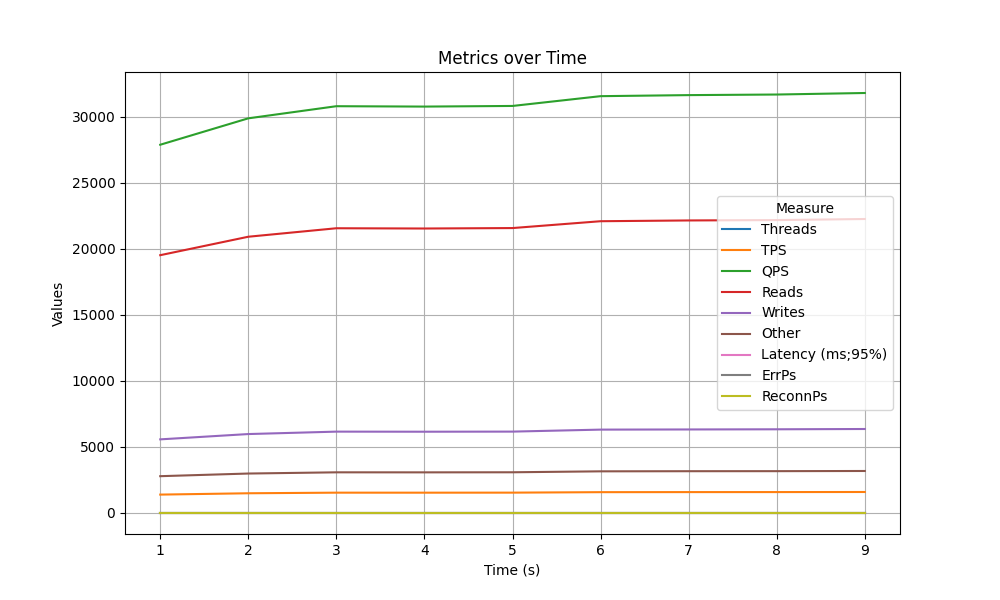
\includegraphics[width=.8\textwidth]{PNGs/Demo/Summary}
    \caption[Pandas - Beispiel]{Grafik generiert mithilfe des Pythontools Pandas}
    \label{demo-pandas}
\end{figure}

\begin{figure}[!ht]
    \centering
    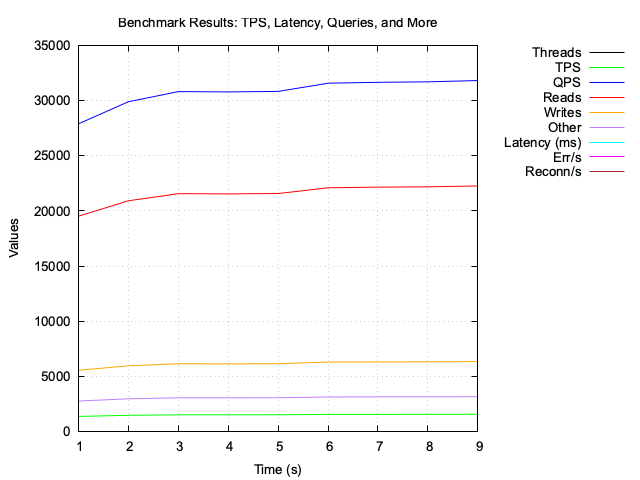
\includegraphics[width=.8\textwidth]{PNGs/Demo/sysbench_output}
    \caption[Gnuplot - Beispiel]{Grafik generiert mithilfe von Gnuplot}
    \label{demo-gnuplot}
\end{figure}


\begin{itemize}
    \item \textbf{Threads}: Die Anzahl der gleichzeitig verwendeten Threads.
    Mehr Threads können die Parallelität erhöhen, jedoch kann eine zu hohe Anzahl
    die Leistung beeinträchtigen, wenn das System überlastet wird.
    \item \textbf{TPS (Transactions Per Second)}: Die Anzahl der Transaktionen pro Sekunde.
    Ein höherer Wert deutet auf eine bessere Datenbankleistung hin.
    \item \textbf{QPS (Queries Per Second)}: Die Anzahl der Abfragen pro Sekunde.
    Ein höherer Wert ist besser und zeigt die Effizienz bei der Verarbeitung von Abfragen.
    \item \textbf{Reads}: Die Anzahl der Leseoperationen.
    Mehr Leseoperationen sind im Allgemeinen besser, da sie eine höhere Datenauslastung anzeigen, was jedoch auch vom spezifischen Anwendungsfall abhängt.
    \item \textbf{Writes}: Die Anzahl der Schreiboperationen.
    Ähnlich wie bei den Leseoperationen: Mehr Schreibvorgänge sind besser, solange die Performance erhalten bleibt.
    \item \textbf{Other}: Bezieht sich auf andere Arten von Operationen, die weder als Reads noch als Writes kategorisiert werden.
    Ein höherer Wert ist gut, solange er nicht zu einer Überlastung führt.
    \item \textbf{Latency (ms; 95\%)}: Die durchschnittliche Zeit in Millisekunden, die benötigt wird, um Anfragen zu bearbeiten, wobei der Wert im 95. Perzentil betrachtet wird.
    Niedrigere Werte sind besser, da sie auf schnellere Reaktionszeiten hinweisen.
    \item \textbf{ErrPs (Errors Per Second)}: Die Anzahl der Fehler pro Sekunde.
    Ein niedriger Wert ist wünschenswert, da er auf eine höhere Stabilität und Zuverlässigkeit des Systems hinweist.
    \item \textbf{ReconnPs (Reconnects Per Second)}: Die Anzahl der Wiederverbindungen pro Sekunde.
    Ein niedrigerer Wert ist ebenfalls besser, da häufige Wiederverbindungen auf Stabilitätsprobleme hindeuten können.
\end{itemize}

%! Author = danielmendes
%! Date = 05.01.25
\chapter{Tools}\label{sec:tools}

\section{Auswahl der Tools}\label{sec:auswahl-der-tools}

Die Grundlage für diese Bachelorarbeit ist das Verhalten der MySQL – Datenbank \cite{sysbench_mysql} in Bezug auf die unterschiedlichen Aspekte, die im Rahmen dieser Arbeit behandelt werden.
Der folgende Abschnitt beschäftigt sich mit Umsetzung, um dieses Verhalten messbar und veranschaulich mithilfe von Grafiken zu machen.
Damit wir die Kennzahlen für bestimmte Abfragen an die MySQL – Datenbank bestimmen können, brauchen wir ein zentrales Tool.
Dieses Tool ist dafür verantwortlich ist die Benchmark - Tests durchzuführen.

Meine Entscheidung ist dabei schlussendlich auf Sysbench \cite{sysbench_repo} gefallen.
Sysbench ist ein Open-Source-Tool, das ein skriptfähiges, multi-threaded Benchmark-Tool ist, das auf LuaJIT basiert.
Es wird hauptsächlich für Datenbankbenchmarks verwendet, kann jedoch auch dazu eingesetzt werden, beliebig komplexe Arbeitslasten zu erstellen, die keinen Datenbankserver erfordern.
Sysbench analysiert dabei Metriken, wie unter anderem Transaktionen pro Sekunde, Latenz und Anzahl an Threads.
Dabei kann man genauer spezifizieren, wie oft diese Metriken geloggt werden sollen.
Sysbench ist dabei nicht auf ein einziges Datenbanksystem eingeschränkt, sondern man kann sich zwischen vielen unterschiedlichen Systemen entscheiden.

Im Zuge der Wahl des Benchmark – Tools habe ich auch andere Benchmarking-Tools betrachtet, wie beispielsweise Benchbase \cite{DifallahPCC13} oder mybench \cite{mybench_repo}.
Im Vergleich zu diesen Tools bietet Sysbench jedoch die Vorteile der höheren Skriptfähigkeit und Flexibilität.
Damit ist gemeint, dass bei Sysbench das erste Projekt mit mehr Aufwand verbunden ist als bei den Alternativen.
Wenn man aber ein Projekt erstmal erstellt hat, dann ist es sehr individuell und man kann schnelle Änderungen hervornehmen.
In dem Kapitel (TODO (Daniel): Kapitel mit Join Typ) betrachten wir ein beispielhaftes Projekt mit Sysbench, bei dem der Einfluss von unterschiedlichen Datentypen als Join-Operator zwischen zwei Tabellen verglichen wird.
Wenn wir später die Performance von unterschiedliche Index-Typen betrachten, dann müssen wir nur an wenigen Stellen Veränderungen durchführen, die in dem Kapitel genauer besprochen werden.

Ein weiterer Vorteil von Sysbench ist, dass es als de facto Standard im Bereich der Datenbankbenchmarks angesehen wird \cite{mybench_comparison}.
Durch diese Position gibt es viele aktive Nutzer und dadurch bedingt viele verfügbaren Ressourcen.
Vorteile der anderen Tools sind jedoch die weniger präzise Steuerung der Ergebnisraten und der Transaktionen von Sysbench.
Zudem ist Sysbench auf das Minimale beschränkt, was den Output angeht, da es, wie schon erwähnt, nur eine Reihe von Log-Dateien gibt und
die Visualisierung der Ergebnisse muss vom Benutzer selbst mithilfe von anderen Tools umgesetzt werden.
Anders sieht dies bei dem Tool mybench aus, da es dort die Möglichkeit gibt in Echtzeit umfassende Abbildungen zu betrachten \cite{mybench_user_interface}.
Obwohl dieses Feature sehr hilfreich ist, bin ich nach Abwägung der Vor- und Nachteile zu dem Entschluss gekommen, dass die einfachere Bedienung und die Tatsache,
dass Sysbench der de facto Standard ist, für mich überwiegen, weshalb ich mich für Sysbench entschieden habe.

Nichtsdestotrotz kann nicht komplett auf Graphen verzichtet werden, da Entwicklungen im Laufe einer Zeitmessung in einem Kurvenverlauf deutlich besser zu erkennen sind als in einer Log - Datei.
Anhand der reinen Zahlen lassen sich unter Umständen Trends von zwei oder etwas mehr unterschiedliche Messungen erkennen, aber besonders wiederkehrende Trends werden aus der schriftlichen Form nicht schnell ersichtbar.
Ganz anders sieht dies bei Graphen mit einer Zeitachse aus.
Dort werden sofort Trends ersichtlich und auch der Vergleich zwischen den unterschiedlichen Messungen erfolgt deutlich besser.

Um die Kennzahlen, die mithilfe von Sysbench ermittelt worden sind, in eine grafische Darstellung umzuwandeln, gibt es unterschiedliche Tools, die wiederum einige Vor - und Nachteile mit sich bringen.
Das erste mögliche Tool stellt Gnuplot \cite{gnuplot} dar, mit dem sich CSV – Dateien sehr gut darstellen lassen.
Wenn man aber nur bestimmte Spalten aus der Tabelle darstellen lassen, dann kommt man schnell an seine Grenzen.
Deshalb habe ich mich für eine anpassungsfähigere Alternative entschieden, denn die Transformationen und die grafische Darstellung wird mithilfe eines Python Scripts umgesetzt.
Für die grafische Darstellung sind dabei die Libraries pandas \cite{reback2020pandas} und matplotlib.pyplot \cite{hunter_2007} verantwortlich.

\section{Einführung in die Tools}\label{sec:einfuhrung-in-die-tools}

Als allererstes muss der MySQL – Server gestartet sein.
Dabei ist es egal, ob dies lokal auf dem Rechner oder über einen Docker in eines GitHub CI/CD-Workflows erfolgt.
Das Wichtigste dabei ist es, dass man sich die Zugangsdaten, bestehend aus User - und Passwortdaten, zwischen speichert, da diese gebraucht werden, um den Benchmarktest mit Sysbench zu starten.
Nachdem das RDBMS gestartet worden ist, muss zudem eine Datenbank erstellt werden.
Dies könnte unter anderem so aussehen:

\lstinputlisting[
    language=sql,
    caption=Create Database,
    label={lst:create_db},
    style=custom_daniel,
]{Scripts/Tools/01_database.sql}

Nach der erfolgreichen Erstellung der Datenbank muss das Tool Sysbench installiert werden.
Um sich mit dem Tool Sysbench vertraut zu machen, gehen wir die verschiedenen Argumente, die beim Aufruf mitgegeben können oder müssen, durch.
Darunter gehören:

\begin{itemize}
    \item \texttt{--db-driver}: Gibt den Treiber für die Datenbank an, die Sysbench verwenden soll. In diesem Fall \texttt{mysql}, um die MySQL-Datenbank zu testen.
    \item \texttt{--mysql-host}: Der Hostname oder die IP-Adresse des MySQL-Servers. Standardmäßig wird \texttt{localhost} verwendet, wenn nichts angegeben wird.
    \item \texttt{--mysql-user}: Der Benutzername, mit dem Sysbench auf die MySQL-Datenbank zugreift.
    \item \texttt{--mysql-password}: Das Passwort für den MySQL-Benutzer. Falls der Benutzer kein Passwort hat oder der Zugriff über eine andere Authentifizierungsmethode erfolgt, kann dieses Argument weggelassen werden.
    \item \texttt{--mysql-db}: Der Name der MySQL-Datenbank, auf die zugegriffen wird. In diesem Beispiel \texttt{sbtest}.
    \item \texttt{--time}: Gibt die Laufzeit des Benchmarks in Sekunden an und muss immer mit angegeben werden.
    \item \texttt{--report-interval}: Gibt das Intervall in Sekunden an, in dem Zwischenergebnisse während des Tests ausgegeben werden.
    Sofern \texttt{--report-interval} nicht gesetzt wird, werden die Ergebnisse nur am Ende des Tests angezeigt.
    \item \texttt{--tables}: Die Anzahl der Tabellen, die für den Test erstellt werden sollen. Standardmäßig wird nur eine Tabelle erstellt.
    \item \texttt{--table-size}: Die Anzahl der Datensätze (Zeilen) pro Tabelle. Muss auch nicht zwingend angegebend werden.
\end{itemize}

Neben den sieben aufgelisteten Argumenten gibt es zwei weitere wichtige Optionen:
\begin{enumerate}
    \item Wie im Abschnitt (\ref{itm:mehrere_selects}) erwähnt, kann ein Lua-Skript angegeben werden, um eigene
    Tabellen zu erstellen, Beispieldaten einzufügen und bestimmte Abfragen durchzuführen.
    Dazu muss am Ende der Sysbench-Befehlszeile lediglich der Pfad zur Lua-Datei hinzugefügt werden.
    Ein erklärendes Beispiel dazu folgt weiter unten in diesem Abschnitt.
    \item Die Methode, den Sysbench ausführen soll, muss ebenfalls spezifiziert werden.
    Auch dieser wird am Ende der Sysbench-Befehlszeile angehängt.
\end{enumerate}

Zunächst schauen wir ein kurzes Demo-Beispiel, denn es gibt die Möglichkeit die Datenbank
auf Performance zu testen, ohne selbst eigene SQL-Befehle zu schreiben. Dafür gibt es vordefinierte Testtypen von Sysbench.
Auf diese Weise kann man schnell die Korrektheit der Einrichtung des Tools überprüfen, bevor man Lua-Scripts
für die eigenen Bedürfnisse schreibt.

Man kann unter anderen zwischen diesen Testtypen wählen:
\begin{itemize}
    \item \textbf{oltp\_insert}: Prüft die Fähigkeit der Datenbank, Daten schnell und effizient einzufügen und
    simuliert eine Umgebung, in der viele Schreiboperationen ausgeführt werden.
    \item \textbf{oltp\_read\_only}: Fokussiert sich auf die Performance bei Leseoperationen und
    eignet sich, um die Leistung bei einer rein lesenden Arbeitslast zu testen.
    \item \textbf{oltp\_read\_write}: Simuliert eine realistische Arbeitslast, bei der sowohl Lese- als
    auch Schreiboperationen gleichzeitig durchgeführt werden.
\end{itemize}

Des Weiteren gibt es auch unterschiedliche Methoden, die mit den Testtypen kombiniert werden können.

\begin{itemize}
    \item \textbf{prepare}: Bereitet die Datenbank für den Test vor, u.a. das Erstellen von benötigten Tabellen.
    \item \textbf{run}: Ist die Ausführungsphase des Tests. Je nach Testtyp führt diese Methode die spezifizierten Operationen aus,
    wie etwa das Einfügen von Daten (oltp\_insert), das Abfragen von Daten (oltp\_read\_only) oder beides (oltp\_read\_only).
    Dabei wird die Performance der Datenbank unter der angegebenen Arbeitslast gemessen.
    \item \textbf{cleanup}: Diese Methode sorgt dafür, dass nach Abschluss des Tests alle Testdaten entfernt werden.
    Sie stellt die Datenbank in ihren ursprünglichen Zustand zurück und stellt sicher,
    dass keine Testdaten zurückbleiben, die eine mögliche produktive Umgebung beeinträchtigen könnten.
\end{itemize}

Für das Demo-Beispiel wählen wir den Testtypen \textbf{oltp\_read\_write} und allen Methoden aus.
Für die Methode run würde unsere Query so aussehen, wobei \texttt{YOUR\_USER} und \texttt{YOUR\_PASSWORD}
entsprechend ersetzt werden müssten:

\begin{lstlisting}[style=custom_daniel,label={lst:sysbenchrun}]
sysbench oltp_read_write \
  --db-driver=mysql \
  --mysql-user=YOUR_USER \
  --mysql-password=YOUR_PASSWORD \
  --mysql-db="sbtest" \
  --time=10 \
  --report-interval=1 \
  run
\end{lstlisting}

Wenn man nur diese Query ausführt, fällt er auf, dass die Query scheitert.
Die Fehlermeldung lautet dabei wie folgt:
\begin{lstlisting}[style=custom_daniel,label={lst:error_withoutprepare}]
FATAL: MySQL error: 1146 "Table 'sbtest.sbtest1' doesn't exist"
\end{lstlisting}
Der entstandene Fehler wird offensichtlich dadurch verursacht, dass die Tabelle nicht erstellt worden ist.
Die Lösung für dieses Problem ist die Ausführung der \texttt{prepare} - Methode vor der \texttt{oltp\_read\_write} - Methode.
Damit sich die Datenbank wieder im Anfangszustand befindet noch anschließend an die \texttt{oltp\_read\_write} - Methode noch die \texttt{cleanup} aufrufen werden.
Um sich die manuelle Ausführung dieser drei Befehl in der korrekten Reihenfolge zu sparen, bietet es sich an, ein Shell-Script zu schreiben, indem zuerst die Methoden nacheinander aufgerufen werden.

\lstinputlisting[
    language=bash,
    caption=Process of Sysbench commands,
    label={lst:sysbench_monitor},
    style=custom_daniel,
    basicstyle=\ttfamily\scriptsize,
]{Scripts/Tools/02_process_sysbench.sh}

Die Ergebnisse werden nun der Log-Datei (unter output/sysbench.log) gespeichert.
Damit fehlt uns nur noch die Erstellung der Graphen.
Um uns diese Erstellung zu vereinfachen, bietet es sich an, dass aus der Log - Datei die entsprechende Kennzahlen extrahiert und die Werte mit korrekten Spaltenüberschriften in einer CSV-Datei speichert.
Dies geht mit dem Shell - Kommando \texttt{grep}:

\lstinputlisting[
    language=bash,
    caption=Extraction from log to CSV,
    label={lst:extraction_csv},
    style=custom_daniel,
    basicstyle=\ttfamily\scriptsize,
]{Scripts/Tools/03_extraction_csv.sh}

Als letzten Schritt gibt es die Erstellung der Graphen mithilfe von der Tools Gnuplot oder der Python - Library Pandas.
Die kompletten Scripts \texttt{plot\_sysbench.gp} und \texttt{generatePlot.py} befinden sich am Ende dieser Bachelorarbeit.
Das Python-Script, das zuständig ist für die Graphgenerierung muss als Argument zum einen
die CSV-Datei übermittelt bekommen und zum anderen kann es nur eine bestimmte Auswahl an
Messwerten übergeben, damit nur für diese die Graphen erzeugt werden.

\lstinputlisting[
    language=bash,
    caption=Generation of graphs,
    label={lst:graph_generation},
    style=custom_daniel,
    basicstyle=\ttfamily\scriptsize,
]{Scripts/Tools/04_graph_generation.sh}

\begin{figure}[!ht]
    \centering
    \begin{subfigure}[t]{0.48\textwidth}
        \centering
        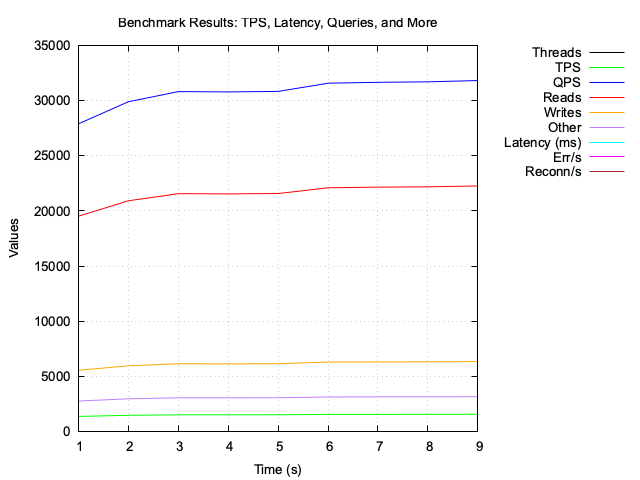
\includegraphics[width=\textwidth]{PNGs/Demo/sysbench_output}
        \label{demo-gnuplot}
    \end{subfigure}
    \hfill
    \begin{subfigure}[t]{0.48\textwidth}
        \centering
        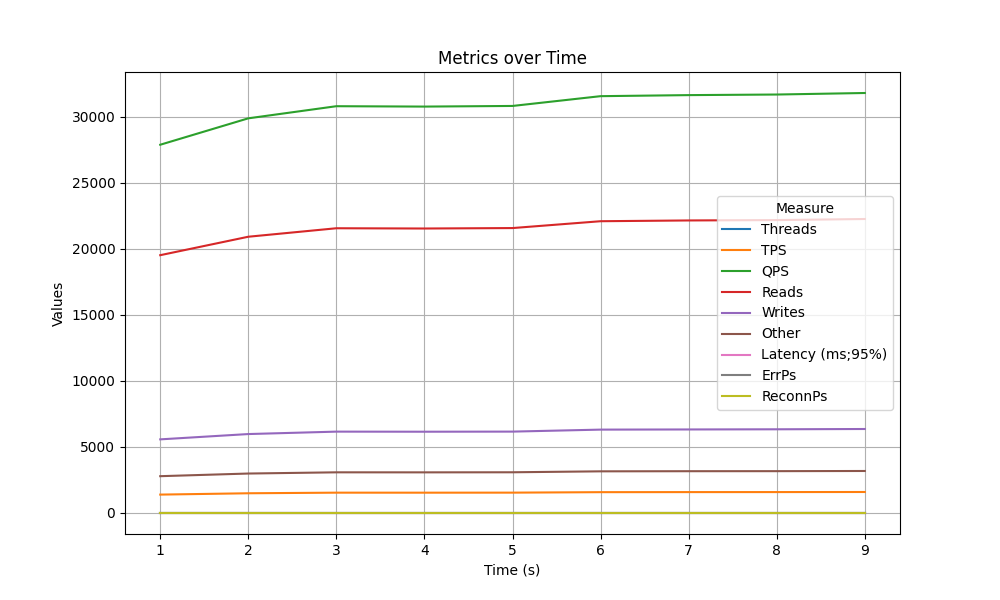
\includegraphics[width=\textwidth]{PNGs/Demo/Summary}
        \label{demo-pandas}
    \end{subfigure}
    \caption[Demo-Graphs: Gnuplot vs. Pandas]{Die Grafik zeigt die erstellten Graphen mit Gnuplot (links) und Pandas (rechts)}
    \label{fig:demo-graph-generation}
\end{figure}


\begin{itemize}
    \item \textbf{Threads}: Die Anzahl der gleichzeitig verwendeten Threads.
    Mehr erhöhen die Parallelität, jedoch zu viele können zur Überlastung des Systems führen.
    \item \textbf{TPS (Transactions Per Second)}: Die Anzahl der Transaktionen pro Sekunde.
    Ein höherer Wert deutet auf eine bessere Datenbankleistung hin.
    \item \textbf{QPS (Queries Per Second)}: Die Anzahl der Abfragen pro Sekunde.
    Ein höherer Wert ist besser und zeigt die Effizienz bei der Verarbeitung von Abfragen.
    \item \textbf{Reads}: Die Anzahl der Leseoperationen.
    \item \textbf{Writes}: Die Anzahl der Schreiboperationen.
    \item \textbf{Other}: Bezieht sich auf andere Arten von Operationen, die weder als Reads noch als Writes kategorisiert werden.
    \item \textbf{Latency (ms; 95\%)}: Die durchschnittliche Zeit in Millisekunden, die benötigt wird, um Anfragen zu bearbeiten, wobei der Wert im 95. Perzentil betrachtet wird.
    Niedrigere Werte sind besser, da sie auf schnellere Reaktionszeiten hinweisen.
    \item \textbf{ErrPs (Errors Per Second)}: Die Anzahl der Fehler pro Sekunde.
    Ein niedriger Wert weist auf höhere Stabilität und Zuverlässigkeit des Systems hin.
    \item \textbf{ReconnPs (Reconnects Per Second)}: Die Anzahl der Wiederverbindungen pro Sekunde.
    Häufige Wiederverbindungen können auch auf Stabilitätsprobleme hindeuten.
\end{itemize}

\section{Genauere Darstellung anhand eines Beispiels}\label{sec:genauere-darstellung-anhand-eines-beispiels}
In dem vorausgegangenen Kapitel \nameref{sec:einfuhrung-in-die-tools} wurde das Tool Sysbench und seine Funktionsweise anhand eines Demo - Projekts näher erläutert.
Damit die Reihenfolge und die Bedeutungen der unterschiedlichen Methoden (prepare → run → cleanup) sowie die Vorgehensweise zur Erstellung unserer Grafiken deutlich geworden.
Das bisherige Problem ist aber, dass wir bei dem dargelegten Beispiel keine Kontrolle über die getesteten Daten haben.
Wenn man sich die Logs genauer anschaut, dann sieht man, dass man über die Parameter an den Sysbench – Befehl die Anzahl der erstellten Tabellen und eingefügten Datensätze von außen steuern kann, aber die genaue Implementierung können wir auf diese Weise nicht steuern.
Genau für diese Anwendungsfälle gibt es die Möglichkeit ein Lua - Skript als Parameter beim Sysbench - Aufruf mit anzugeben.
In diesen Lua - Dateien können die Implementierungen der einzelnen Methoden selbstständig gewählt werden.

Um das Vorgehen besser erklären zu können, schauen wir uns dafür ein Beispiel an.
Für das Beispiel wollen wir zwei Tabellen erstellen und anschließend mit zufälligen Testdaten befüllen.
Die Abfrage, die wir auf Performance testen wollen, ist das Verbinden (Joinen) dieser beiden Tabellen.
In unserem Fall wollen wir eine Kundentabelle erstellen, die Informationen wie Name, Geburtstag und Adresse enthält, sowie eine Bestelltabelle, die Details wie Artikelnummer, Bestelldatum usw. speichert und einen Bezug zu dem Kunden herstellt, der die Bestellung aufgegeben hat.
Damit wir aber nicht nur ein Beispiel haben, das dargestellt wird, brauchen wir einen Vergleich zwischen zwei verschiedenen Implementierungen.
Dieser Unterschied zwischen den beiden Implementierungen besteht darin, dass in der einen Version die Tabelle eine Kundennummer vom Typ \texttt{Int} enthält, während in der anderen keine Kundennummer vorhanden ist.
Stattdessen wird in der Bestelltabelle auf den Namen (Typ \texttt{Varchar}) verwiesen.
Da Verbundoperationen zu den aufwendigsten Operationen gehören, gehen wir davon aus, dass der kleine Typ \texttt{Int} Performancevorteile gegenüber der anderen Version hat.
Dies gilt es nun mit den Benchmarktest genauer zu untersuchen.

Für die Durchführen der Benchmarks beginnen wir zunächst unabhängig von Sysbench und den Lua – Skripten mit der Spezifizierung der Tabellen, die erstellt werden sollen.
Dies müssen wir einmal mit der Kundennummer und einmal mit dem Namen als Fremdschlüssel der Bestelltabelle machen.
Damit müssen insgesamt vier unterschiedliche Create Table - Befehle umgesetzt werden.
So sehen die Create Table für den Fall mit der Kundennummer aus:

\lstinputlisting[
    language=sql,
    caption=Create Table - Befehl für Tabelle Kunden,
    label={lst:create_table_kunde},
    style=custom_daniel,
]{Scripts/Join_Type/01_Create_Table_Kunde.sql}

\lstinputlisting[
    language=sql,
    caption=Create Table - Befehl für Tabelle Bestellung,
    label={lst:create_table_bestellung},
    style=custom_daniel,
]{Scripts/Join_Type/02_Create_Table_Bestellung.sql}

Anschließend müssen wir diese Befehle in \texttt{prepare()} - Funktion miteinbinden.
Dafür müssen wir einfach die Create Table - Befehle an die Datenbank senden.
Wenn wir bestimmte Indexe oder andere Datenbankstrukturen erstellen wollen würden, dann müssten wir dies ebenfalls in dieser Funktion machen.
Dies ist ein Auszug aus der \texttt{Prepare} - Funktion:

\lstinputlisting[
    language={[5.0]Lua},
    caption=Lua - Script für die Erstellung der Tabellen,
    label={lst:prepare_query},
    style=custom_daniel,
    basicstyle=\ttfamily\scriptsize,
]{Scripts/Join_Type/03_Prepare_Query.lua}

Wenn die Datenbank beispielsweise in einer Produktivumgebung läuft, dann wollen wir, dass die Benchmarks möglichst wenig Einfluss aus sie haben.
Damit ist es das Ziel, dass die Datenbank möglichst wieder in ihrem Anfangszustand ist.
Außerdem sollte der Benchmark beliebig oft nacheinander ausgeführt werden können, ohne zu Problemen zu führen.
Wenn wir aber eine Tabelle erstellen und nicht wieder löschen, dann würde im nächsten Durchlauf der Create Table - Befehl scheitern.
Lösen könnte man dies über Klausel „IF NOT EXITS“ bei der Erstellung der Tabelle hinzufügen oder noch es besser ist es die Tabelle am Ende des Benchmarks einfach zu löschen.
Dafür ist die \texttt{cleanup()} – Funktion vorgesehen:

\lstinputlisting[
    language={[5.0]Lua},
    caption=Lua - Script für das Aufräumen,
    label={lst:cleanup_query},
    style=custom_daniel,
    basicstyle=\ttfamily\scriptsize,
]{Scripts/Join_Type/04_CleanUp_Query.lua}

Wichtig ist dabei, dass man keine Schlüsselintegritäten verletzt.
Da in diesem Fall die Tabelle \texttt{BESTELLUNGMITID} eine Referenz auf die Tabelle \texttt{KUNDENMITID} hat, muss zuerst die Bestelltabelle und danach erst die Kundentabelle entfernt werden.

Jetzt haben wir das Gerüst für die eigentlichen Insert - und Select - Befehle geschaffen.
Bei den Insert - Befehlen können wir entweder mit zufälligen Zahlen die Werte generieren oder wir setzen Listen von Namen fest, aus denen zufällig gewählt werden kann.
Da wir jedoch keine Kontrolle über diese zufällig erstellten Werte haben, müssen wir beim Insert - Befehl die Bedingung „Insert Ignore“ hinzufügen, damit doppelte Schlüsselwerte ignoriert werden und keine Fehler verursachen.
Wir müssen hier auch festlegen, wie viele Datensätze für die Kunden erstellt werden und wie viele Bestellungen pro Kunden es geben soll.
Später werden wir noch eine Möglichkeit kennen lernen, um diese Werte von außen zusteuern.
Um sicherzustellen, dass keine Werte in den Tabellen enthalten sind, können wir alle Datensätze aus den Tabellen entfernen, bevor wir sie hinzufügen.
Damit die Performance der Insert – Query auch gemessen wird, ist es wichtig, dass die \texttt{insert()} - Funktion in der \texttt{event()} – Funktion aufgerufen wird.
Sonst kommt es zu diesem Fehler:
\begin{lstlisting}[style=custom_daniel,label={lst:error_withoutevent}]
FATAL: cannot find the event() function in Join.lua
\end{lstlisting}

\lstinputlisting[
    language={[5.0]Lua},
    caption=Lua - Script für das Einfügen von Daten,
    label={lst:insert_query},
    style=custom_daniel,
    basicstyle=\ttfamily\scriptsize,
]{Scripts/Join_Type/05_Insert_Query.lua}

Die letzte Anweisung, die wir noch brauchen, ist die Select - Abfrage.
Hierbei muss man sich Gedanken machen, welche Abfrage benötigt wird, damit die untersuchten Effekte auch tatsächlich auftreten.
In dem Beispiel brauchen wir deswegen einen Join zwischen den beiden Tabellen über den Fremdschlüssel.

\lstinputlisting[
    language={[5.0]Lua},
    caption=Lua - Script für das Abfragen von Daten,
    label={lst:select_query},
    style=custom_daniel,
    basicstyle=\ttfamily\scriptsize,
]{Scripts/Join_Type/06_Select_Query.lua}

Damit haben wir für unseren Vergleich alle vier Operationen genauer definiert und müssen diese 4 Funktionen nur noch leicht anpassen für die Implementierung mit dem Namen als Fremdschlüssel und ohne die Kundennummer in der Kundentabelle.
Daraufhin benötigen wir noch ein Skript, dass die Operationen in der korrekten Reihenfolge ausführt und die Grafiken generiert.
Wichtig dafür ist die folgende Dateienstruktur, die anhand der Int - Verbunds dargestellt wird.

Damit wir die unterschiedlichen Operationen voneinander trennen können, gibt es folgende Dateienstruktur: Es gibt einen Ordner mit einem beliebigen Namen, z.B. \texttt{int\_queries}, in diesem Ordner befinden sich folgende Dateien:
\begin{itemize}\label{files_structure}
    \item \texttt{int\_queries.lua} $\Rightarrow$ enthält die \texttt{prepare()}- und \texttt{cleanup()}-Funktionen
    \item \texttt{int\_queries\_insert.lua} $\Rightarrow$ enthält die \texttt{insert()}-Funktion
    \item \texttt{int\_queries\_select.lua} $\Rightarrow$ enthält die \texttt{select()}-Funktion
\end{itemize}

Analog muss auch ein Ordner für die Varchar - Vergleich erstellt werden.
Als Letztes brauchen wir nur einen Orchestrator, der das korrekte Lua - Skript ausführt, die Ergebnisse in die richtige Log - Datei schreibt und anschließend die CSV - Dateien und die Grafiken erstellt.
Dieser Orchestrator ist das Shell - Skript: \texttt{sysbench\_script.sh}.

Zudem möchten wir unser Beispiel erweitern, da es auch möglich sein soll, unterschiedliche Längen von Varchar hinzuzufügen.
Dadurch könnten wir nicht nur den Performanceunterschied zwischen Int und Varchar feststellen, sondern auch noch den Einfluss der Länge des Verbundoperators für Varchar.
Dazu benötigen wir eine Hilfsfunktion in \texttt{varchar\_queries\_insert.lua}, die einen zufälligen Namen mit der Länge von einer vorgegebenen Zahl erstellt.
Dieser Name ist damit kein natürlicher Name, sondern einfach eine Kombination von zufälligen Buchstaben, aber für unseren Testfall gehen wir diesen Kompromiss ein.
Wenn wir jetzt zwei unterschiedlichen Längen für Varchar testen wollen, dann müssten wir den Varchar - Ordner mit den oben beschriebenen drei Dateien kopieren und nur die Zeile ändern, die die Länge des zufälligen Namens bestimmt.
Dies würde zu extremer Redundanz führen, weshalb man beim Aufruf des Orchestrator - Scripts, Variablen definieren kann, die im Skript selbst exportiert und in der \texttt{varchar\_queries\_insert.lua} - Datei importiert werden können.

Dies ist die Zeile mit der festgelegten Länge:
\begin{lstlisting}[language={[5.0]Lua},label={lst:without_imported_length}]
local length = 10
\end{lstlisting}

Die Zeile mit der importierten Länge:
\begin{lstlisting}[language={[5.0]Lua},label={lst:with_imported_length}]
local length = tonumber(os.getenv("LENGTH"))
\end{lstlisting}

Den Orchestrator - Script ruft man wie folgt auf:
\lstinputlisting[
    language=sh,
    caption=Befehl zum Ausführen des Orchestrator Skripts,
    label={lst:orchestrator_command},
    style=custom_daniel,
]{Scripts/Join_Type/07_Orchestrator_Command.sh}

Die Parameter haben folgende Funktion:
\begin{itemize}[label=--]
    \item \texttt{-out}: Gibt den Pfad an, an welchen der Output-Ordner gespeichert werden soll
    \item \texttt{-var}: Angabe der Variablen und deren Werte, die exportiert werden sollen im JSON-Format
    \item \texttt{-scripts}: Angabe der Pfade zu den Ordnern, die die Lua-Skripte enthalten. Nach dem Doppelpunkt wird angegeben, welche Variable das Skript benötigt. \texttt{Int\_queries} benötigt keine Variablen, deshalb gibt es auch keinen Doppelpunkt.
\end{itemize}

\label{itm:mehrere_selects}
Die letzte Besonderheit ist es, dass man mehrere Select – Abfragen ohne unterschiedliche Insert - Befehle definieren kann.
Zu einem späteren Punkt in der Bachelorarbeit werden wir zu unterschiedliche Indextypen kommen.
Um zu untersuchen, ob ein bestimmter Indextyp bei Abfragen verwendet wird, müssen wir nur unterschiedliche Selects abfragen.
Die eigentlichen Tabellen und deren Datensätze müssen dabei nicht immer wieder gleich befüllt werden.
Wenn wir auch unsere Ordnerstruktur mit dem Int - Query Beispiel zurückkommen, dann könnte man anstelle von \texttt{int\_queries\_select.lua} auch einen Ordner erstellen mit den Namen \texttt{int\_queries\_select}.
In diesem Ordner können beliebig viele unterschiedliche Lua - Skripts sein, die select – Funktionen haben.
Dadurch werden alle Select - Befehle auf der gleichen Datenbasis verglichen und so können wir im Kapitel (TODO (Daniel): Index) erkennen, wann der Index verwendet wird und wann nicht.

Bevor wir uns das Ergebnis des Befehls anschauen, kommen wir zu der Funktionsweise des Orchestrator - Skript \texttt{sysbench\_script.sh}.
Im Grundlegenden arbeitet dieses Skript ähnlich wie schon das Skript im Demo - Beispiel, aber durch die zusätzlichen Anwendungsfälle kommt es zu mehr Komplexität.

Zu Beginn des Skripts werden die Umgebungsvariablen aus der Datei \texttt{db.env} geladen.
Die Variablen helfen zum einen wie bei dem Demo - Beispiel bei die Datenbank - Verbindung und zum anderen können sich auch die Parameter der Benchmarks verändern.
Danach werden die Parameter, die an das Skript übergeben wurden, überprüft.
Beispielsweise wird sichergegangen, dass die für die Skripts verwendeten Parameter, bei unserem Beispiel length für varchar, tatsächlich auch definiert worden sind mit \texttt{-var}.

Wenn wir den Befehl ausführen, wird der Output-Ordner an der gewünschten Stelle erstellt.
In diesem Ordner werden verschiedene Grafiken generiert, die die Ergebnisse visualisieren.
Dabei gibt es zwei unterschiedliche Arten von Grafiken.
Die erste Art von Grafik ist ein Zeitreihendiagramm, welches auf der x-Achse den zeitlichen Verlauf zeigt.
Auf der y-Achse werden in einigen Diagrammen die unterschiedlichen Metriken für jedes einzelne Skript dargestellt, während andere Diagramme die Werte einer bestimmten Metrik auf der y-Achse zeigen und dabei die Ergebnisse verschiedener Skripte vergleichen.
Dadurch können beispielsweise die Metriken \texttt{Reads} und \texttt{Writes} analysiert werden, um herauszufinden, welches Skript in diesen Bereichen besser abschneidet.
Danach wird der Output - Ordner erstellt und die Spaltenüberschriften in die CSV – Dateien geschrieben.
Danach beginnt erst das eigentliche Durchgehen der unterschiedlichen Skripte, die unter dem Argument -script angegeben wurden.
Zunächst schreibt man die einzelnen Dateien nach dem obigen Schema (\ref{files_structure}) auf, denn als Argument wurde nur der oberste Ordner angegeben.
Als nächstes kommt eine Fallunterscheidung, die überprüft, ob dieses Skript exportierte Variable nutzt oder nicht.
Für den Fall, dass keine Variablen exportiert werden (z.B. \texttt{int\_queries}) wird einfach die Prepare – Funktion aufgerufen, dann \texttt{process\_script\_benchmark} und anschließend die Cleanup - Funktion.
Wenn aber Variablen exportiert werden, dann müssen weitere Zwischenschritte umgesetzt werden.
Und zwar müssen alle Kombinationen zwischen den verschiedenen exportierten Variablen generiert werden.
Wenn es drei Variablen gibt, von denen 2 jeweils 2 Werte und eine letzte nur einen Wert hat, dann gibt es 2 * 2 * 1 = 4 unterschiedliche Kombinationen.
Als nächstes muss man für alle diese Kombinationen die Schritte ausführen, die man schon bei der Variante ohne exportierte Variable ausgeführt hat und dabei darf man nicht vergessen die Variablen an sich zu exportieren.

\lstinputlisting[
    language=sh,
    caption=Ausschnitt aus Orchestrator Script,
    label={lst:main_loop},
    style=custom_daniel,
    basicstyle=\ttfamily\scriptsize,
]{Scripts/Join_Type/08_Main_Loop.sh}

Die Funktion \texttt{process\_script\_benchmark} überprüft noch es sich bei dem Select – Directory um einen Ordner handelt oder nicht.
Wenn es ein Ordner ist, dann werden alle Dateien in diesem Ordner mit Sysbench durchgeführt, wenn nicht, dann wird an den Ordner nur die Endung \texttt{.lua} hinzugefügt.

\lstinputlisting[
    language=sh,
    caption=Methode Process Script Benchmark,
    label={lst:process_script_benchmark},
    style=custom_daniel,
    basicstyle=\ttfamily\scriptsize,
]{Scripts/Join_Type/09_Process_Script_Benchmark.sh}

Die Methode \texttt{run\_benchmark} führt den Sysbench – Befehl aus und wenn es sich um die Methode \texttt{Run} handelt, dann müssen die Daten während der Ausführung und die Statistiken am Ende in je eine CSV - Datei speichern.
Aus diesen beiden CSV - Dateien müssen die Insert - und Select - Queries der zugehörigen Skripte wieder vereint werden und die Attribute werden miteinander addiert.
Als letzter Schritt erfolgt noch der bekannte Schritt der Grapherstellung.

\lstinputlisting[
    language=sh,
    caption=Methode Run Benchmark,
    label={lst:run_benchmark},
    style=custom_daniel,
    basicstyle=\ttfamily\scriptsize,
]{Scripts/Join_Type/10_Run_Benchmark.sh}

INFO: Die Shell - Ausschnitte sind zum Teil verkürzt und würden auf diese Weise nicht funktionieren.

Wenn wir den Befehl ausführen, wird der Output-Ordner an der gewünschten Stelle erstellt.
In diesem Ordner werden verschiedene Grafiken generiert, die die Ergebnisse visualisieren.
Die erste Art stellen Zeitreihendiagramme dar, die auf der X-Achse den zeitlichen Verlauf zeigen.
Auf der Y-Achse werden hingegen in einigen Diagrammen die unterschiedlichen Metriken eines einzelnen Skripts dargestellt, während andere Diagramme die Werte einer bestimmten Metrik auf der Y-Achse zeigen und dabei die Ergebnisse verschiedener Skripte vergleichen.
Dadurch können beispielsweise die Metriken "Reads" und "Writes" analysiert werden, um herauszufinden, welches Skript in diesen Bereichen besser abschneidet.

Die zweite Art von Grafik, die erstellt wird, ist ein Hexagon - Diagramm.
Dieses verzichtet auf eine Zeitachse und fasst die Performance über den gesamten Zeitraum hinweg zusammen.
Im Vergleich zur Laufzeitanalyse liefert es zusätzliche Informationen, wie etwa die Latenz oder die Gesamtanzahl der Queries.
Dadurch ist es auch möglich, dass mehrere Skripte und mehrere Kennzahlen in einer Grafik dargestellt werden können.

PNGs

\begin{figure}[!ht]
    \centering
    \begin{subfigure}[t]{0.48\textwidth}
        \centering
        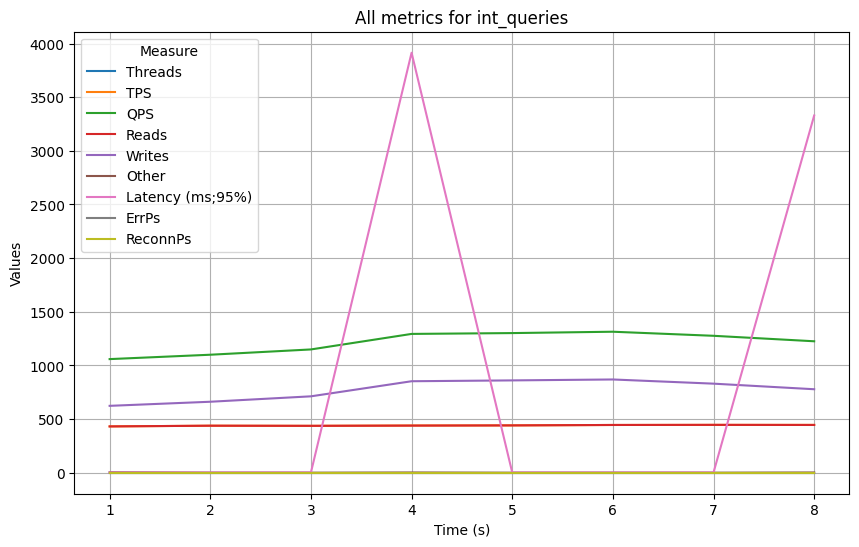
\includegraphics[width=\textwidth]{PNGs/Join_Type/int_queries}
        \label{join-typ-int_queries}
    \end{subfigure}
    \hfill
    \begin{subfigure}[t]{0.48\textwidth}
        \centering
        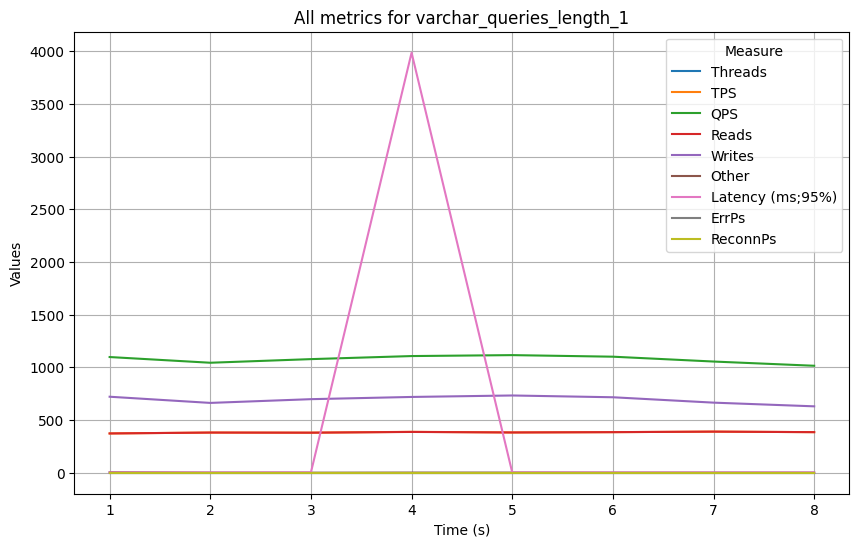
\includegraphics[width=\textwidth]{PNGs/Join_Type/varchar_queries_length_1}
        \label{join-typ-varchar_queries_length_1}
    \end{subfigure}
    \caption[Join-Typ: Skriptvergleich]{Die Grafik zeigt alle Metriken für die Skripte \texttt{int\_queries} (links) und \texttt{varchar\_queries\_length\_1} (rechts)}
    \label{fig:join-typ-comp-script}
\end{figure}

\begin{figure}[!ht]
    \centering
    \begin{subfigure}[t]{0.48\textwidth}
        \centering
        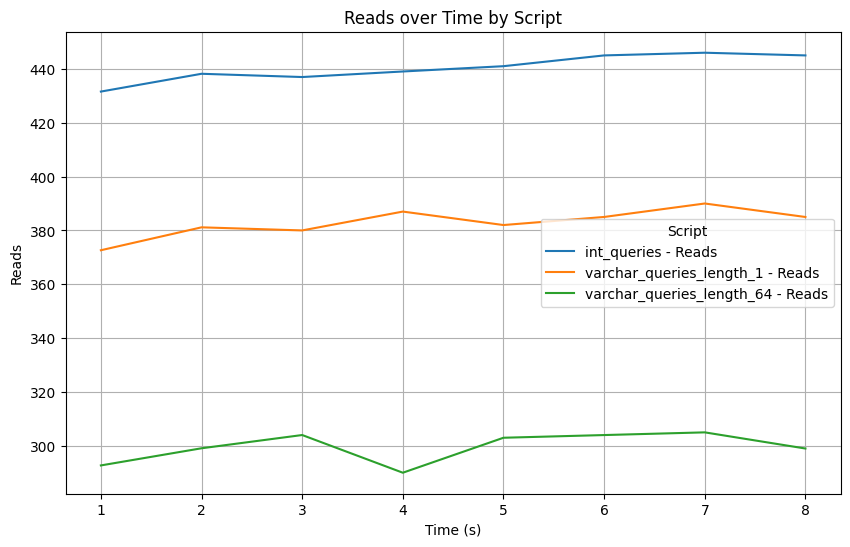
\includegraphics[width=\textwidth]{PNGs/Join_Type/Reads}
        \label{join-typ-reads}
    \end{subfigure}
    \hfill
    \begin{subfigure}[t]{0.48\textwidth}
        \centering
        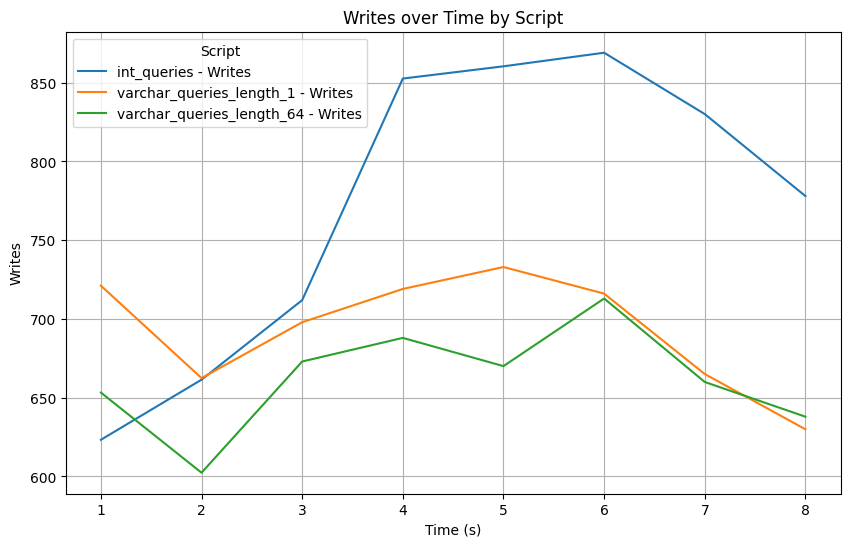
\includegraphics[width=\textwidth]{PNGs/Join_Type/Writes}
        \label{join-typ-writes}
    \end{subfigure}
    \caption[Join-Typ: Metrikvergleich]{Die Grafik zeigt den Vergleich zwischen allen Skripten für die Metriken Reads (links) und Writes (rechts)}
    \label{fig:join-typ-comp-metric}
\end{figure}

\begin{figure}[!ht]
    \centering
    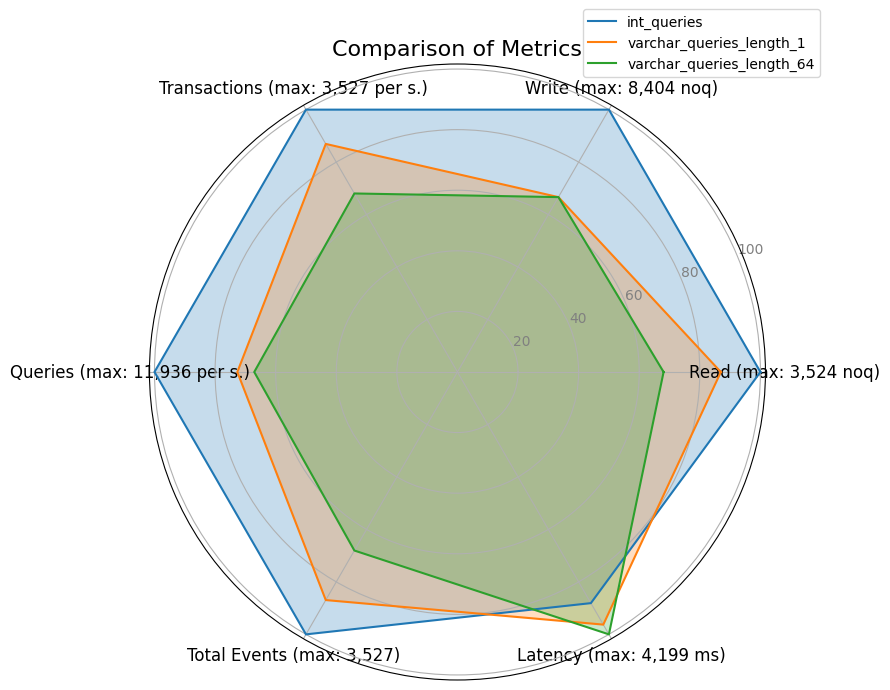
\includegraphics[width=.7\textwidth]{PNGs/Join_Type/statistics}
    \caption[Join-Typ: Hexagon-Diagramm]{Darstellung der Skripte und 6 Metriken in einem Hexagon}
    \label{fig:join-typ-hex}
\end{figure}

Aus den Grafiken, die für ein Skript alle Metriken veranschaulichen, kann man möglicherweise Datenfehler erkennen.
So springt bei Abbildung (\texttt{int\_queries.png}) die Latenz bei einigen Messpunkten von 0 ms auf einen deutlich erhöhten Wert und danach wieder auf 0 ms zurück.
Ansonsten aber sind die anderen Metriken auf einem konstanten Level, und es gibt wenige Schwankungen.
Bei der Abbildung (\texttt{varchar\_queries\_length\_1.png}) sieht dies sehr ähnlich aus, und auch dort schwankt die Latenz etwas mehr.
Wenn wir jetzt die drei Skripte miteinander vergleichen wollen, können wir die Abbildungen Reads.png und Writes.png heranziehen.
Was die Lesegeschwindigkeit angeht, kann man erkennen, dass \texttt{int\_queries} am meisten Reads hat, als Nächstes kommt \texttt{varchar\_queries\_length\_1} und dann \texttt{varchar\_queries\_length\_64}.
Damit sind die Abfragen, wie wir erwartet haben, bei \texttt{int\_queries} am schnellsten, und je länger der String wird, desto langsamer werden die Abfragen.
Bei den Schreibgeschwindigkeiten sieht das schon etwas anders aus, wobei es hier zunächst bei allen eine langsamere Startphase gibt.
Anschließend an diesen Cold Start liegt das Niveau von \texttt{int\_queries} am höchsten, also auch am schnellsten.
Die beiden \texttt{varchar\_queries} sind hier aber überraschenderweise auf einem ähnlichen Niveau.
Bei der Abbildung (\texttt{statistics.png}) kann man die Effekte der Lese- und Schreibgeschwindigkeiten auch erkennen.
Es fällt auch auf, dass, anders als bei Reads, Writes, Queries, die Latenz bei schnelleren Queries geringer ist und nicht der höchste Wert der Beste ist.
%! Author = danielmendes
%! Date = 29.11.24

\chapter{Optimierungen von Datentypen}

Das erste Thema, das wir in Bezug auf die Performance - Optimierung von Datenbanken betrachten, sind die unterschiedlichen Datentypen und ihre Effizienzsteigerungen.
Bei der Auswahl des korrekten Datentyps gibt es unterschiedliche Faktoren, die vom jeweiligen Typen abhängen.
Es gibt aber auch allgemeinere Prinzipien, die auf fast alle Datentypen angewendet werden können.

\section{Allgemeine Faktoren}

Bei der Erstellung von Tabellen sollte man folgende Schritte für die Auswahl von Datentypen befolgen.
Zunächst muss die allgemeine Klasse der Typen, wie beispielsweise numerisch, Zeichenketten oder zeitbezogen, festgelegt werden.
Anschließend sollte der spezifische Typ ausgewählt werden.
Für numerische Daten kommen beispielsweise Ganzzahlen wie \texttt{INT} oder Fließkommazahlen wie \texttt{FLOAT} und \texttt{DOUBLE} infrage.
Die spezifischen Typen können dieselbe Art von Daten speichern, unterscheiden sich jedoch im Bereich der Werte, die sie speichern können.
Auch sind sie unterschiedlich in der Precision (Genauigkeit), die sie erlauben und dem physischen Speicherplatz, den sie entweder auf der Festplatte oder im Arbeitsspeicher benötigen.
Einige Datentypen haben auch spezielle Verhaltensweisen und Eigenschaften.

Allgemein gilt für Datentypen, dass kleiner besser ist, weshalb man den kleinstmöglichen Datentypen wählen sollte, den man speichern kann und der die vorhandenen Daten entsprechend repräsentieren kann.
Dadurch wird zum einen weniger Speicherplatz (In-Memory und CPU-Cache) in Anspruch genommen, was meistens zu schnelleren Abfragen führt.
Zum anderen spricht für die Benutzung von kleinstmöglichen Typen die einfache Typveränderung.
Wenn die vorhandenen Daten falsch eingeschätzt wurden und nachträglich ein größerer Datentyp benötigt wird, kann der Typ ohne größere Probleme vergrößert werden.
Eine weitere allgemeine Richtlinie ist die Einfachheit von Datentypen.
Damit ist beispielsweise gemeint, dass Integer einfach zu verarbeiten ist als Character, weshalb man immer einen Integer wählen sollte, wenn man durch ihn die Daten korrekt abbilden kann.
Dies liegt daran, dass weniger CPU-Zyklen benötigt werden, um Operationen auf einfacheren Datentypen zu verarbeiten.
Bei dem Beispiel mit Integer und Character liegt dies an den Character Sets und Sortierregeln, die den Character-Vergleich erschweren.

Die letzte allgemeine Regel, die Performancegewinne bringt, ist die Vermeidung von \texttt{NULL}.
Viele Tabellen enthalten NULLABLE Spalten, selbst wenn die Anwendung kein NULL (Fehlen eines Wertes) speichern muss, da dies die Standardeinstellung ist.
Daher ist es am besten solche Spalten bei der Tabellenerstellung mit dem Identifier \texttt{NOT NULL} zu definieren.
Wenn allerdings \texttt{NULL}-Werte gespeichert werden sollen, dann sollte der Identifier nicht genutzt werden.
Für MySQL ist es dann schwieriger Abfragen zu optimieren, da dadurch Indizes, Indexstatistiken und Wertevergleiche mehr Speicherplatz benötigen und komplizierter werden.
Dies liegt daran, dass indizierte nullable Spalten ein zusätzliches Byte pro Eintrag gebrauchen, was dazu führen kann, dass ein Index mit fester Größe in einen variablen Index umgewandelt wird.
Allerdings fällt die Leistungssteigerung, die durch die Änderung von \texttt{NULL}-Spalten in \texttt{NOT NULL} erzielt wird, in der Regel gering aus.
Besonders bei Verwendung von Indizes sollte aber darauf geachtet werden.

MySQL unterstützt auch viele Aliase, z.B. \texttt{INTEGER}, \texttt{BOOL}, \texttt{NUMERIC}.
Diese Aliase können verwirrend sein, aber sie beeinflussen nicht die Performance.
Wenn eine Tabelle mit einem aliasierten Datentyp erstellt wird und die Tabelle mit SHOW CREATE TABLE untersucht wird, fällt auf, dass statt des aliasierten Datentyps der Basistyp angezeigt wird, da der aliasierte Datentyp intern in den Basistyp umgewandelt wurde.

\section{Einzelne Datentypen und weitere Faktoren}
Bevor wir untersuchen, ob die eben beschriebene Prinzipien tatsächlich einen Einfluss auf die Performance haben, müssen die speziellen Verhaltensweisen der bekanntesten Datentypen betrachtet werden.

Für nummerische Datentypen gibt es die Wahl zwischen Ganzzahlen und Fließkommazahlen.
Die spezifischen Typen unterscheiden sich nur in der Anzahl der Bits, die sie speichern können.
\texttt{SMALLINT} kann 16 Bits speichern, während \texttt{INT} 32 und \texttt{BIGINT} 64 Bits speichern kann.
Dementsprechend verändert sich auch der mögliche Wertebereich der Zahlen, die durch den Speicherplatz abgedeckt sind.
Mit den optionalen \texttt{UNSIGNED} - Attribute können keine negativen Werte gespeichert werden können, dafür verdoppelt sich aber die obere Grenze der Positiven.
Zeitgleich bleiben der Speicherplatz und die Leistung gleich.
Die Berechnung der Wertebereiche für den default, bzw. mit den Signed - Attribut, erfolgt in \ref{eq:equation-signed} und mit dem Unsigned - Attribut in \ref{eq:equation-unsigned}.

\vspace{-4mm}
\begin{gather}
    \text{Signed: } -2^{(N-1)} \text{ bis } 2^{(N-1)} - 1\label{eq:equation-signed} \\
    \text{Unsigned: } 0 \text{ bis } 2^N - 1\label{eq:equation-unsigned}
\end{gather}

\textbf{Hinweis:} $N$ entspricht der Anzahl der Bits.
\vspace{4pt}

Beispiel für 8 Bits:
\begin{itemize}
    \item \text{SIGNED:} -128 \text{ bis } 127
    \item \text{UNSIGNED:} 0 \text{ bis } 255
\end{itemize}

Eine Breitenangabe wie \texttt{INT(11)} beeinflusst nur die Anzeige und nicht den Wertebereich oder die Speicheranforderungen.
Um dies zu beweisen, können wir die folgende Table erstellen.

\lstinputlisting[
    language=sql,
    caption=SQL-Befehl zur Erstellung der Testtabelle,
    label={lst:testint_create_sql},
    style=custom_daniel,
]{Scripts/Datatypes/01_testint_create.sql}

Da wir den für die beiden Variablen den Typen INT gewählt haben und wir überprüfen wollen, ob die Breitenangabe einen Einfluss auf die Speicheranforderungen hat, können wir die Grenzen des Wertebereichs für INT einfügen: -2147483648 und 2147483647.
\lstinputlisting[
    language=sql,
    caption=Inserts und Selects für Testtabelle aus \ref{lst:testint_create_sql},
    label={lst:testint_queries_sql},
    style=custom_daniel,
]{Scripts/Datatypes/02_testint_queries.sql}

\begin{table}[h!]
    \centering
    \caption{Ergebnis der SQL-Abfrage aus \ref{lst:testint_queries_sql}}
    \begin{tabular}{|c|c|}
        \hline
        \textbf{int\_5} & \textbf{int\_11} \\ \hline
        2147483647 & 2147483647 \\ \hline
        -2147483648 & -2147483648 \\ \hline
    \end{tabular}
    \label{tab:int_values}
\end{table}
Für den maximalen Wert von INT werden 32 Bits benötigt: $2^{(32-1)} - 1 = 2147483647$.
INT(5) und INT(11) können beide die Grenzwerte von INT speichern, weshalb wir bestätigt haben, dass die Breitenangabe keinen Einfluss auf die Speicheranforderungen hat, ansonsten hätten wir einen Fehler bei der Einfügung der Werte bekommen.

Ein spezifischer Typ für eine Festkommazahl ist \texttt{DECIMAL}, die auch für die Speicherung von Ganzzahlen geeignet ist.
Außerdem kann man bei einer Festkommazahl auch die Genauigkeit angeben, da die maximale Anzahl der Ziffern vor und nach dem Dezimalpunkt definiert werden.
\texttt{DECIMAL(18, 9)} beispielsweise speichert neun Ziffern vor und nach dem Dezimalpunkt und benötigt dafür 9 Bytes Speicherplatz.
\texttt{DECIMAL} speichert Zahlen in einer binären Zeichenkette (binary string) mit neun Ziffern pro vier Bytes und unterstützt bis zu 65 Ziffern insgesamt.

Zu den Fließkommazahlen gehören die \texttt{FLOAT}- und \texttt{DOUBLE}-Typen, die die standardmäßige Gleitkomma-Arithmetik verwenden und für ungefähre Berechnungen optimiert sind.
\texttt{FLOAT} benötigt 4 Bytes, während \texttt{DOUBLE} 8 Bytes Speicherplatz beansprucht und eine höhere Präzision sowie einen größeren Wertebereich bietet.
Die Gleitkomma-Arithmetik ist aufgrund der nativen Verarbeitung durch die CPU deutlich schneller als die präzise Berechnung mit \texttt{DECIMAL}, bringt jedoch einen gewissen Präzisionsverlust mit sich.
Alternativ kann auch \texttt{BIGINT} genutzt werden, um sowohl die Ungenauigkeit von Gleitkomma-Speicherungen als auch die höheren Kosten der \texttt{DECIMAL}-Arithmetik zu vermeiden.

Die beiden Haupttypen für Zeichenketten sind \texttt{VARCHAR} und \texttt{CHAR}. \texttt{VARCHAR} speichert die Zeichenfolgen mit variabler Länge und benötigt daher weniger Speicherplatz als Typen mit fester Länge, da nur so viel Platz verwendet wird, wie tatsächlich benötigt wird.
Zusätzlich werden ein oder zwei Bytes für die Speicherung der Länge der Zeichenfolge verwendet (1 Byte für < 255 Bytes Zeichenfolge).
Durch diese effiziente Speichernutzung ist VARCHAR der am häufigsten verwendete Datentyp für Zeichenketten, aber es hat auch Nachteile, da Aktualisierungen an den Werten zu wachsenden Zeilen und damit auch zusätzliche Verarbeitung der Speicher - Engine erfordern kann.
Und obwohl die Speicherung von \texttt{hello} in \texttt{VARCHAR(5)} oder \texttt{VARCHAR(200)} gleich viel Speicherplatz benötigt, kann es trotzdem ineffizienter für Sortierungen oder Operationen auf temporären Tabellen sein.
Deshalb sollte trotzdem immer so viel Platz reserviert werden, wie tatsächlich benötigt wird.

\texttt{CHAR} hingegen hat eine feste Länge und MySQL reserviert immer auch den nicht gebrauchten Platz für die angegebene Anzahl an Zeichen.
Daher ist \texttt{CHAR} ideal für sehr kurze Strings oder Werte, die alle nahezu gleich lang sind, da \texttt{VARCHAR(1)} zwei Bytes aufgrund des Längen - Bytes benötigt, \texttt{CHAR(1)} hingegen auch.
Außerdem ändert sich bei CHAR die Speicherstruktur bei Aktualisierungen nicht, weshalb dieser Datentyp besser geeignet ist, wenn die Daten häufig verändert werden.
Hingegen \texttt{VARCHAR} eignet sich besonders, wenn die maximale Länge einer Spalte deutlich größer ist als die durchschnittliche Länge der gespeicherten Werte.

\texttt{DATETIME} und \texttt{TIMESTAMP} können dieselbe Art von Daten speichern und beide haben dabei eine Genauigkeit von einer Sekunde.
\texttt{TIMESTAMP} benötigt aber nur halb so viel Speicherplatz, ist zeitzonenbewusst und verfügt über spezielle Auto-Update-Funktionen.
Allerdings hat \texttt{TIMESTAMP} einen viel kleineren Bereich an erlaubten Werten und manchmal können seine speziellen Fähigkeiten ein Nachteil sein.

\section{Analyse der Benchmarks}

Der erste Leitsatz, den wir untersuchen, besagt, dass Spalten nach Möglichkeit als \texttt{NOT NULL} deklariert werden sollten.
Für den Nachweis benutzen wir erneut die Kundentabelle (\ref{lst:create_table_kunde}).
Diesmal erstellen wir eine Tabelle, bei der das Attribut \texttt{NOT NULL} für alle Spalten deklariert wird, sowie eine Tabelle ohne dieses Attribut.
Wenn das Attribut nicht deklariert wird, dann können u.a. auch \texttt{NULL}-Werte in die Tabelle eingefügt werden.

\vspace{-15pt}
\begin{figure}[H]
    \centering
    \begin{subfigure}[t]{0.48\textwidth}
        \centering
        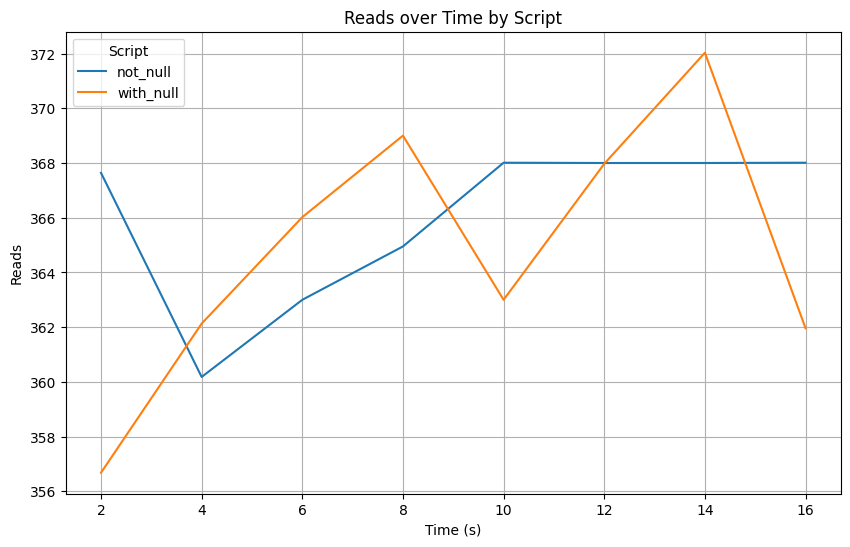
\includegraphics[width=\textwidth]{PNGs/Script/Data_Types/Null/null-check/Reads}
        \caption{Readsabfragen für jeweils 2 Selects}
        \label{data-types-null-reads}
    \end{subfigure}
    \hfill
    \begin{subfigure}[t]{0.48\textwidth}
        \centering
        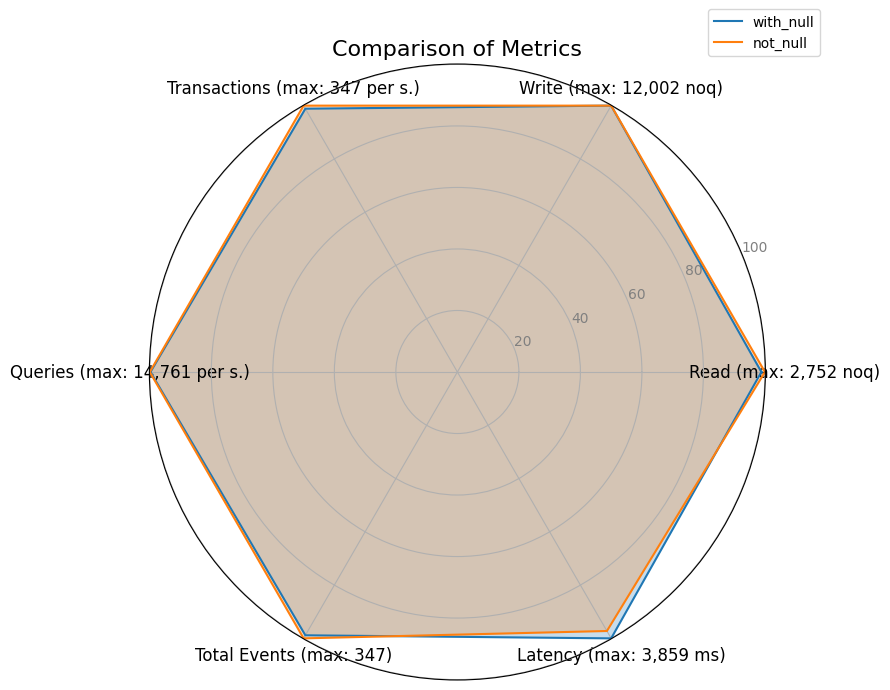
\includegraphics[width=\textwidth]{PNGs/Script/Data_Types/Null/null-check/statistics}
        \caption{Metriken über den kompletten Zeitraum}
        \label{fig:data-types-null-statistics}
    \end{subfigure}
    \caption{Vergleich von NULL und NOT NULL}
\end{figure}
\vspace{-20pt}

In der erstellten Grafik (siehe Abbildung \ref{data-types-null-reads}) sind die beiden Resultate der Select-Befehle zu sehen, die sowohl einfache WHERE-Klauseln als auch Count- und Group-By-Befehle enthalten.
Anhand der Grafik lässt sich erkennen, dass die Werte für \texttt{NOT NULL} höher liegen als für \texttt{NULL}, bzw \texttt{WITH NULL}.
Höhere Werte bedeuten, dass mehr Abfragen pro Sekunde durchgeführt werden können, was auf eine bessere Performance hindeutet.
Deshalb lässt es sich sagen, dass \texttt{NOT NULL} besser performt als \texttt{NULL}, aber wenn man auf die Y-Achse schaut, fällt auf, dass die Werte nicht so weit auseinanderliegen, sondern der Unterschied nur marginal ist.
Daher sollten beim Datenbankentwurf Entscheidungen nicht aus Performancegründen getroffen werden, sondern aus Gründen der Datenintegrität und -konsistenz.

Um zu zeigen, dass man bei der Wahl zwischen unterschiedlichen Datentypen, den simpleren wählen sollte, haben wir erneut die Kundentabelle (\ref{lst:create_table_kunde}) benutzt.
Für diesen Vergleich haben wir den Datentyp des Schlüsselattributs der Tabelle geändert, zunächst \texttt{INT} und anschließend \texttt{CHAR}.
An den Ergebnissen fällt auf, dass die Schreibbefehle bei beiden Skripten etwa gleich schnell sind, aber bei den Abfragen gibt es deutliche Unterschiede.
Hier zeigt sich, dass bei Wertevergleichen \texttt{INT} deutlich schneller ist als \texttt{CHAR} (etwa 50\%).
Bei der Sortierung ist die Reihenfolge gleich, jedoch fallen die Abstände deutlich geringer aus (\ref{data-types-simpler-reads}).

\vspace{-15pt}
\begin{figure}[H]
    \centering
    \begin{subfigure}[t]{0.48\textwidth}
        \centering
        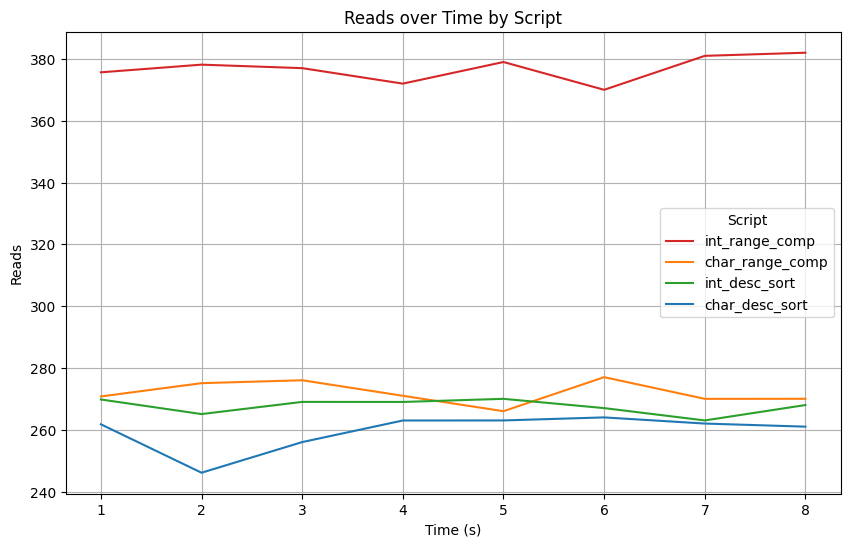
\includegraphics[width=\textwidth]{PNGs/Script/Data_Types/Simpler/int-char/Reads}
        \caption{Vergleich für jeweils 2 unters. Abfragen}
        \label{data-types-simpler-reads}
    \end{subfigure}
    \hfill
    \begin{subfigure}[t]{0.48\textwidth}
        \centering
        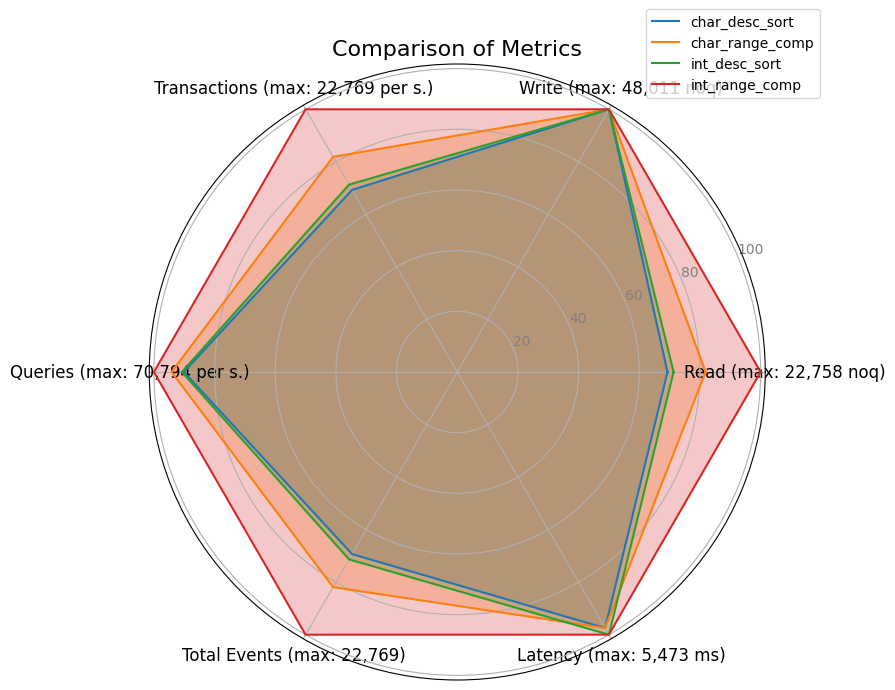
\includegraphics[width=\textwidth]{PNGs/Script/Data_Types/Simpler/int-char/statistics}
        \caption{Kennzahlen über den gesamten Zeitraum}
        \label{fig:data-types-simpler-statistics}
    \end{subfigure}
    \caption{Vergleich von INT und CHAR}
\end{figure}
\vspace{-20pt}

Als Letztes wollten wir unterschiedliche Datentypen vergleichen.
Dazu haben wir die gleiche Tabelle wie beim Vergleich von \texttt{INT} und \texttt{CHAR} verwendet, jedoch diesmal unterschiedliche numerische oder Zeichenketten-Typen für den Primärschlüssel benutzt.
Beim Vergleich der numerischen Typen zeigt sich, dass \texttt{DECIMAL} mit deutlichem Abstand am langsamsten ist (Abbildung \ref{data-types-smaller-number-type-reads}).
Danach folgt, wie vermutet, der nächstgrößere Datentyp \texttt{BIGINT}.
Auffällig ist, dass der Unterschied zwischen \texttt{INT}, \texttt{MEDIUMINT} und \texttt{SMALLINT} kleiner ist als erwartet.
Dies wird vermutlich aber daran liegen, dass wir die Abfragen nur auf eine Tabelle mit wenigen tausend Datensätzen ausgeführt haben.
In der Produktion mit Hunderttausenden oder Millionen von Datensätzen ist anzunehmen, dass die Unterschiede zwischen den Typen größer wären als in unserem Vergleich.

\vspace{-18pt}
\begin{figure}[H]
    \centering
    \begin{subfigure}[t]{0.48\textwidth}
        \centering
        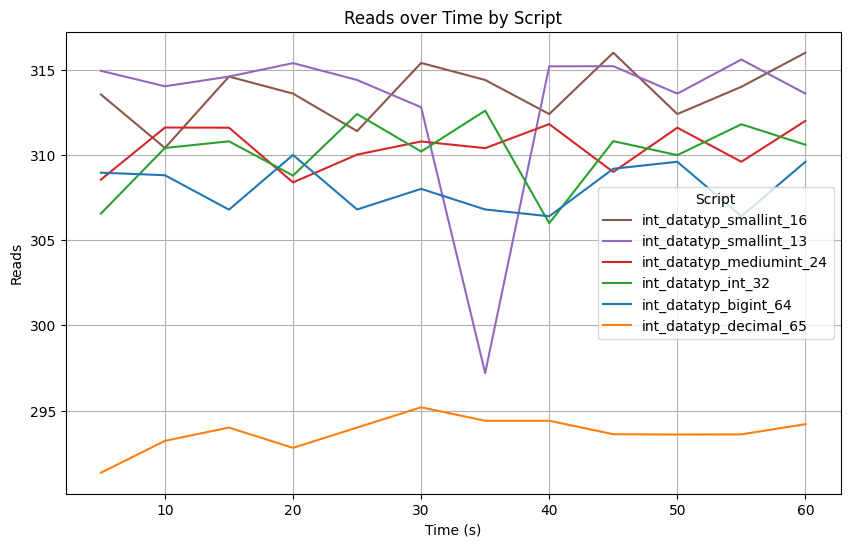
\includegraphics[width=\textwidth]{PNGs/Script/Data_Types/Smaller/number-type/Reads}
        \caption{Unterschiedliche numerische Typen}
        \label{data-types-smaller-number-type-reads}
    \end{subfigure}
    \hfill
    \begin{subfigure}[t]{0.48\textwidth}
        \centering
        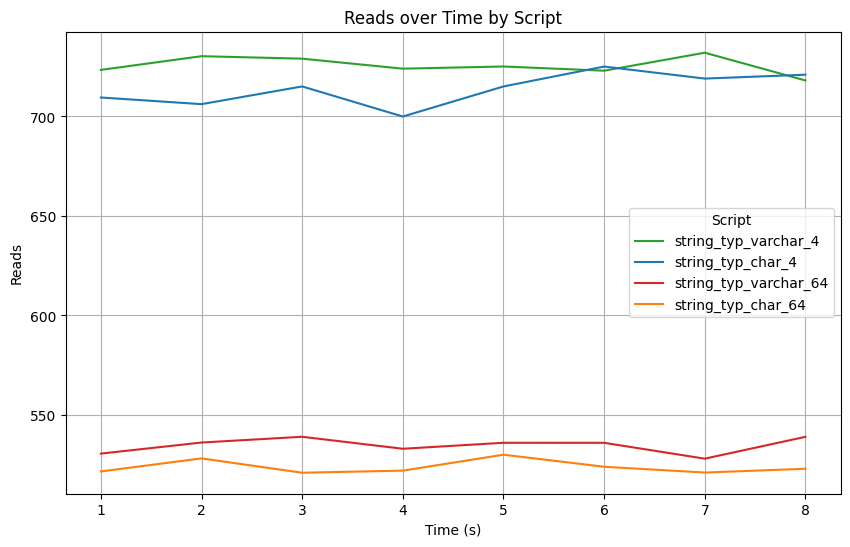
\includegraphics[width=\textwidth]{PNGs/Script/Data_Types/Smaller/string-type/Reads}
        \caption{Unterschiedliche Zeichenketten-Typen}
        \label{fig:data-types-smaller-string-type-reads}
    \end{subfigure}
    \caption{Vergleich von unterschiedlichen Select-Abfragen}
\end{figure}
\vspace{-20pt}

Beim Vergleich zwischen den beiden Zeichenketten-Typen \texttt{CHAR} und \texttt{VARCHAR} ist unabhängig von der Länge zu erkennen, dass \texttt{VARCHAR} effizienter ist als \texttt{CHAR} (\ref{fig:data-types-smaller-string-type-reads}).
Im ersten Vergleich wurde jeweils eine Länge von 4 Stellen verwendet und beim zweiten Vergleich eine Länge von 64 Stellen.
Bei beiden untersuchten Längen ist \texttt{VARCHAR} schneller als \texttt{CHAR}.
Wenn man sich jedoch die Performance beim Einfügen von Werten anschaut, fällt auf, dass die Unterschiede eher gering sind und es gibt auch stärkere Schwankungen bei den Werten (siehe Abbildung \ref{fig:data-types-smaller-string-type-writes}).

\vspace{-12pt}
\begin{figure}[H]
    \centering
    \begin{subfigure}[t]{0.48\textwidth}
        \centering
        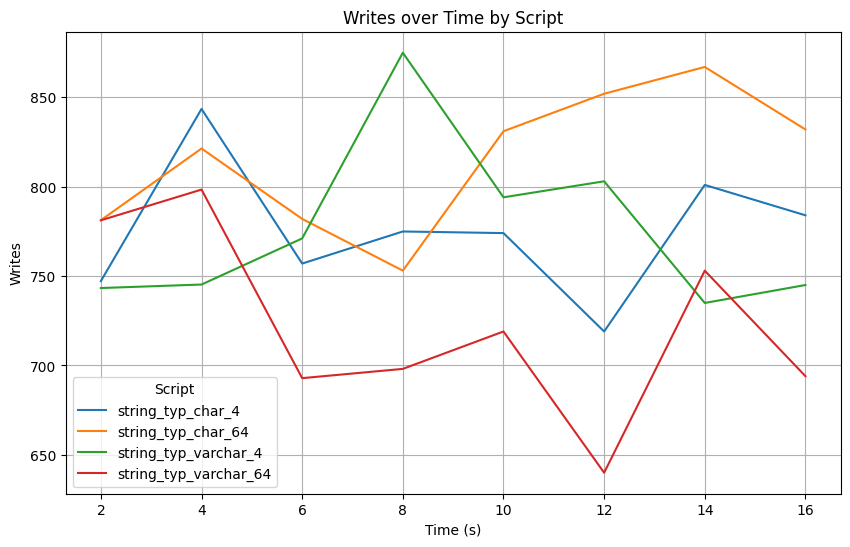
\includegraphics[width=\textwidth]{PNGs/Script/Data_Types/Smaller/string-type/Writes}
        \caption{Bei gleicher Länge der Zeichen}
        \label{fig:data-types-smaller-string-type-writes}
    \end{subfigure}
    \hfill
    \begin{subfigure}[t]{0.48\textwidth}
        \centering
        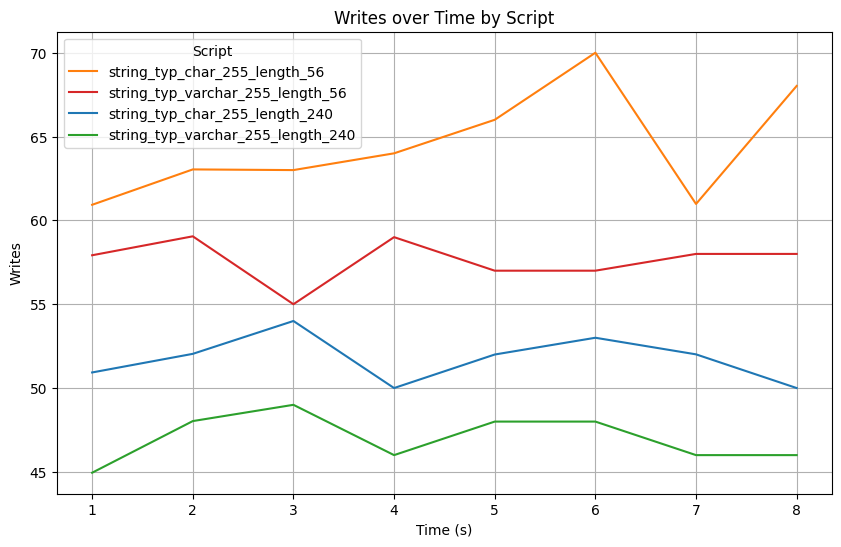
\includegraphics[width=\textwidth]{PNGs/Script/Data_Types/Smaller/string-type-length/Writes}
        \caption{Bei unterschiedlichem Befüllungsgrad}
        \label{fig:data-types-smaller-string-type-length-writes}
    \end{subfigure}
    \caption{Vergleiche von unterschiedlichen Write-Abfragen}
\end{figure}
\vspace{-20pt}

Als letzten Vergleich haben beide Zeichenketten-Typen mit der Länge von 255 Stellen definiert, aber dafür mit unterschiedlich vielen Stellen befüllt.
Anschließend haben wir bei beiden Tabellen die Werte aktualisiert und wenige Stellen bei der Namen-Spalte zufällig hinzugefügt.
Wenn man dies tut, dann fällt auf, dass \texttt{CHAR} schneller ist als \texttt{VARCHAR} (\ref{fig:data-types-smaller-string-type-length-writes}).
Zusätzlich wird der Unterschied zwischen den beiden Typen größer, je mehr Stellen befüllt werden.
Damit haben wir gezeigt, dass die Vorteile von \texttt{CHAR} insbesondere bei der Aktualisierung von Werten liegen, während \texttt{VARCHAR} bei der Selektion von Werten besser abschneidet.
Der Grund hierfür ist, dass \texttt{CHAR} die verbleibenden Stellen mit Leerzeichen auffüllt, was zu einem höheren Speicherbedarf führt.
%! Author = danielmendes
%! Date = 29.11.24

\chapter{Indizes}\label{ch:indexes}

Das folgende Kapitel befasst sich mit der Indexierung und den damit verbundenen Performance-Optimierungen, die näher erläutert werden.
Zunächst werden einige Grundlagen der Indexierung betrachtet.
Anschließend werden die verschiedenen Arten von Indizes näher erläutert und unterschiedliche Benchmarks mit ihnen durchgeführt.
Im letzten Schritt werden die Ergebnisse analysiert, um festzustellen, welche Verwendung der Indizes am besten funktioniert.

\section{Grundlagen}\label{sec:indexing-grundlagen}

Indizes sind Datenstrukturen, die von Speicher-Engines (engl.\ storage engines) verwendet werden, um unter anderem Zeilen schneller zu finden (\cite[S. 147--189]{schwartz2012high}).
Die Storage-Engine ist eine Kernkomponente eines Datenbankmanagementsystems, die für die Speicherung und Verwaltung der Daten verantwortlich ist.
Verschiedene Storage-Engines unterscheiden sich hinsichtlich ihrer Indexfunktionalität sowie der Unterstützung von Transaktionen und Sperrmechanismen.
Im weiteren Verlauf werden verschiedene Indextypen vorgestellt, die nicht von allen Engines unterstützt werden.

Die Indizes haben einen großen Einfluss auf die Datenbank-Performance und werden mit zunehmender Größe der Datenbank immer wichtiger, da das Scannen aller Tupel zunehmend aufwendiger wird.
Weniger ausgelastete Datenbanken können ohne ordnungsgemäße Indizes gut funktionieren, aber die Leistung kann rapide sinken, wenn die Datenmenge wächst.
Wenn ein solches Problem auftritt, ist die Index-Optimierung oft der effektivste Weg, um die Abfrageleistung schnell zu verbessern.
Um wirklich optimale Indizes zu erstellen, ist es häufig notwendig, Abfragen umzuschreiben.
Besonders nützlich sind Indizes bei Abfragen, die Joins zwischen mehreren Tabellen enthalten, da sie ermöglichen, die Anzahl der zu prüfenden Tupel erheblich zu reduzieren, wenn eine einschränkende Bedingung vorliegt.
Wie genau Indizes erstellt werden müssen, wird im Laufe dieses Kapitels geklärt.


Um die Funktionsweise eines Indexes anschaulicher zu erklären, wird als Beispiel ein wissenschaftliches Fachbuch betrachtet.
Am Ende dieser Bücher gibt es meist ein Stichwortverzeichnis oder Register.
Dieses Register besteht aus einer alphabetisch geordneten Liste von Begriffen, Themen und Stichworten.
Möchte man einen Begriff nachschlagen, sucht man ihn im Stichwortverzeichnis und erhält die Seitenzahlen, auf denen er vorkommt.
In DBMS verwendet die Storage-Engine Indizes auf eine ähnliche Weise.
Sie durchsucht die Datenstruktur des Indexes nach einem Wert.
Und wenn ein Treffer gefunden wird, kann die Engine die Zeilen ermitteln, die den Treffer enthalten.
Das folgendes Beispiel veranschaulicht dies:

\begin{lstlisting}[language=SQL]
SELECT NAME FROM KUNDEN WHERE KUNDEN_ID = 7;
\end{lstlisting}

Angenommen, es existiert ein Index auf der Spalte \texttt{KUNDEN\_ID}, dann wird MySQL diesen verwenden, um Zeilen zu finden, bei denen die \texttt{KUNDEN\_ID} den Wert 7 hat.
Mit anderen Worten wird eine Suche innerhalb der Indexwerte durchgeführt und alle entsprechenden Zeilen werden zurückgegeben.

Ein Index kann Werte aus einer oder mehreren Spalten einer Tabelle enthalten.
Bei mehreren Spalten ist die Reihenfolge der Spalten im Index entscheidend, da MySQL nur effizient auf ein linkes Präfix des Indexes zugreifen kann.
Gibt man nur das zweite Attribut an, ohne das erste zu referenzieren, kann der Index nicht direkt verwendet werden.
Außerdem darf man nicht verwechseln, dass ein Index über zwei Spalten nicht gleichbedeutend ist mit zwei separaten einspaltigen Indizes.
Es gibt verschiedene Typen von Indizes, die jeweils für unterschiedliche Zwecke optimiert sind und in den nächsten Abschnitten behandelt werden.

Um zu verstehen, wie man Indizes für eine Datenbank auswählt, ist es wichtig zu wissen, welcher Teil der Abfrage am meisten Zeit in Anspruch nimmt (\cite[S. 350--353]{garcia2008database}).
Das Datenbanksystem ist so aufgebaut, dass die Tupel einer Relation üblicherweise auf viele Seiten einer Festplatte verteilt sind, die jeweils mehrere Tausend Bytes umfassen und viele Tupel speichern.
Um die Werte eines Tupels zu prüfen, muss die gesamte Seite, auch Block genannt, in den Hauptspeicher geladen werden.
Dabei kostet es kaum mehr Zeit, alle Tupel einer Seite anstatt nur ein einzelnes zu prüfen.

In der Regel stellt der Schlüssel den sinnvollsten Index für eine Tabelle dar, weshalb MySQL standardmäßig den B-Tree-Index für Primary Keys verwendet (\cite{mysql_primary_key}).
Die Entscheidung, ob für ein bestimmtes Attribut ein Index definiert werden soll, hängt von drei Faktoren ab:
Erstens ist ein Index besonders nützlich, wenn Abfragen häufig auf ein bestimmtes Attribut zugreifen.
Zweitens kann ein Index sinnvoll sein, wenn es nur wenige Tupel für einen bestimmten Wert des Attributs gibt, da dies den Festplattenzugriff bei einer Abfrage reduziert.
Sobald nicht alle Blöcke geladen werden müssen, kann der Index Zeit sparen.
Der letzte Fall betrifft Situation, in denen Tupel nach einem Attribut geclustert sind.
Durch einen Index können müssen hier weniger Datenblöcke geladenen werden, da die Werte des Attributs aufeinanderfolgender gespeichert sind.
Mit diesen Faktoren kann begründet werden, warum die Schlüssel einer Tabelle gut geeignet sind.
Zum einen kommen sie oft in Abfragen vor (erster Punkt) und zum anderen enthalten sie keine doppelten Werte, da jedes Tupel einen eindeutigen Wert hat (zweiter Punkt).

Das Auswählen von Indizes erfordert von den Entwicklern eine Tradeoff abzuwägen.
Es gibt dabei zwei Faktoren, die die Entscheidung beeinflussen.
Zum einen kann ein Index auf einem Attribut Abfragen mit diesem Attribut erheblich beschleunigen.
Zum anderen erschwert jeder Index Einfügungen, Löschungen und Aktualisierungen, da diese mehr Zeit und Aufwand erfordern.
Aber selbst wenn Modifikationen die häufigste Form von Datenbankaktionen sind, kann ein Index auf ein häufig verwendetes Attribut die Leistung verbessern.
Dies liegt daran, dass einige Modifikationsbefehle zuvor die Datenbank abfragen.
Im Kapitel \nameref{ch:partitions} wird uns dieses Thema wieder begegnen.

Um Zeitersparnis durch die Nutzung von Tupeln ohne vollständige Durchsuchung der Relation zu erreichen, müssen Indizes auf der Festplatte gespeichert werden.
Dies führt jedoch zu zusätzlichen Festplattenzugriffen.
Allgemein lässt sich sagen, dass Modifikationen in etwa doppelt so kostenintensiv sind wie der Zugriff auf den Index oder die Daten während einer Abfrage.
Damit berechnet werden kann, ob sich ein Index für eine Spalte lohnt, muss bekannt sein, mit welcher Wahrscheinlichkeit Abfragen und Modifikationen durchgeführt werden.

Um die Vorgehensweise anhand einer beispielhaften Berechnung durchzuführen, wird die folgende Tabelle benutzt (abgeändertes Beispiel aus~\cite[S. 355--357]{garcia2008database}):
\vspace{-4pt}
\begin{lstlisting}
Fakten(Id, Bestelldatum, Artikel_Id, Kunden_Id, ...)
\end{lstlisting}
\vspace{-8pt}

Der Schlüssel der Faktentabelle ist die Spalte \texttt{Id} und für die Attribute \texttt{Artikel\_Id} sowie \texttt{Kunden\_Id} wird jeweils ein Index erstellt.
Damit stehen uns insgesamt drei unterschiedliche Indexe zur Verfügung, einschließlich des Primärschlüssels.
Als Nächstes werden Befehle benötigt, bei denen die Indexe benutzt werden (siehe~\ref{lst:indexing:fakten-select-insert-queries}).
In der ersten Zeile wird nur der Kundenindex verwendet, in der zweiten nur der Artikelindex und in der Letzten fügen wie eine Zeile ein.

\vspace{-12pt}
\begin{lstlisting}[language=SQL,caption=Select-Queries für die Faktentabelle,label={lst:indexing:fakten-select-insert-queries}]
SELECT Bestelldatum, Artikel_Id FROM Fakten WHERE Kunden_Id = k;
SELECT Bestelldatum, Kunden_Id FROM Fakten WHERE Artikel_Id = a;
INSERT INTO Fakten VALUES(i, b, a, k);
\end{lstlisting}
\vspace{-8pt}

Damit berechnet werden kann, ob es sinnvoll ist, die Indizes zu erstellen, müssen bestimmte Voraussetzungen festgelegt werden.
Zuallererst wird davon ausgegangen, dass die Faktentabelle 10 Datenblöcke belegt und im Durchschnitt jeder Kunde 3 Artikel kauft, während ein Artikel von 3 Kunden gekauft wird.
Die Tupel für einen bestimmten Kunden oder Artikel sind gleichmäßig über die 10 Seiten verteilt.
Trotzdem sind mit einem Index nur 3 Festplattenzugriffe erforderlich, um die durchschnittlich 3 Tupel für einen Kunden oder Artikel zu finden.
Dazu ist ein Festplattenzugriff erforderlich, um die Seite des Indexes zu lesen und ein weiterer, um die modifizierte Seite zurückzuschreiben, falls eine Indexseite geändert werden muss.
Ohne Index sind 10 Festplattenzugriffe zum Lesen und zwei Festplattenzugriffe zum Schreiben erforderlich.
Unter diesen Bedingungen ergibt sich die folgende Kostentabelle:

\vspace{-18pt}
\begin{table}[H]
    \centering
    \setlength{\arrayrulewidth}{0.4mm}
    \[
        \begin{array}{r|c c c c}
            \textbf{Aktion} & \textbf{Kein Index} & \textbf{Kunden Index} & \textbf{Artikel Index} & \textbf{Beide Indizes} \\ \hline
            Q_1 & 10 & 4 & 10 & 4 \\
            Q_2 & 10 & 10 & 4 & 4 \\
            I   & 2  & 4  & 4  & 6 \\ \hline
            \textbf{Durchschnitt} & 2 + 8p_1 + 8p_2 & 4 + 6p_2 & 4 + 6p_1 & 6-2p_1-2p_2 \\
        \end{array}
    \]
    \vspace{-5pt}
    \caption[Performance-Vergleich]{Kosten der unterschiedlichen Queries in Abhängigkeit der Indizes}
    \label{tab:performance-queries}
\end{table}
\vspace{-25pt}

Die letzte Zeile aus Tabelle~\ref{tab:performance-queries} gibt die durchschnittlichen Kosten einer Aktion an.
Unter der Annahme, dass der Anteil der Zeit, in der die erste Abfrage ausgeführt wird, p1 beträgt und der Anteil der Zeit für die zweite Abfrage p2 ist, ergibt sich der Anteil der Zeit, in der I ausgeführt wird, zu 1 – p1 – p2.
Der Durchschnitt für den Kundenindex wird wie folgt berechnet:
\[
    4p_{1} + 10p_{2} + 4 \cdot (1 - p_{1} - p_{2}) = 4p_{1} + 10p_{2} + 4 - 4p_{1} - 4p_{2} = 4 + 6p_{2}
\]

Abhängig von den Werten für p1 und p2 kann jede der vier Optionen die geringsten Kosten für die drei Operationen verursachen.
Zum Beispiel, wenn p1 = p2 = 0,1, dann ist der Ausdruck 2 + 8p1 + 8p2 am kleinsten, sodass keine Indizes bevorzugt werden würden.
Wenn jedoch p1 = 0,5 und p2 = 0,1 gelten, ergibt ein Index für die Kunden den besten Durchschnittswert.

Damit wurde gezeigt, dass es sinnvoll ist, keinen Index zu verwenden, wenn überwiegend Einfügungen durchgeführt werden und nur sehr wenige Abfragen anfallen.
Intuitiv gilt, dass bei vielen Abfragen und einer ungefähr gleichen Häufigkeit von Abfragen, die Artikel und Kunden angeben, beide Indizes vorteilhaft sind.
Wird hingegen nur ein Typ von Abfrage häufig genutzt, sollte nur der Index definiert werden, der bei dieser Abfrageart hilft.

Es gibt zahlreiche Tools, die entwickelt wurden, um die Verantwortung der Wahl der Indizes vom Datenbankdesigner zu übernehmen.
Dabei optimiert das System sich selbst oder dem Designer werden zumindest Empfehlungen für sinnvolle Entscheidungen gegeben.
Ein bewährter Ansatz zur Auswahl von Indizes ist das sogenannte Greedy-Verfahren (\cite[S. 824]{garcia2008database}), bei dem zunächst ohne ausgewählte Indizes der Nutzen jedes Kandidaten-Index bewertet wird.
Wenn es einen Index mit positivem Nutzen gibt, wird dieser ausgewählt und anschließend wird eine Neubewertung ausgeführt, wobei davon ausgegangen wird, dass der zuvor ausgewählte Index bereits verfügbar ist.
Dieser Prozess wird so lange wiederholt, bis es keinen Kandidaten-Index mit positivem Nutzen mehr gibt.

\newpage
\section{B-Baum-Index}\label{sec:indexing-b-baum-index}

Der erste zu betrachtende Indextyp ist der B-Baum-Index (engl.\ B-Tree Index), der auf einer speziellen Baum-Datenstruktur basiert.
Diese Struktur wird von den meisten MySQL-Storage-Engines unterstützt.
Die Implementierung und Nutzung des B-Baum-Indexes kann jedoch je nach verwendeter Storage-Engine variieren.

Das Grundprinzip eines B-Baums ist, dass alle Werte in einer bestimmten Reihenfolge gespeichert werden und jede Blattseite den gleichen Abstand zum Wurzelknoten hat.

\begin{quote}
    \enquote{The height of a B+ tree depends on the number of data entries and the size of index entries.} (\cite[S. 358]{ramakrishnan2002database})
\end{quote}

Ein B-Baum-Index beschleunigt den Datenzugriff, da die Storage-Engine nicht die gesamte Tabelle durchsuchen muss, um die gewünschten Daten zu finden.
Stattdessen beginnt die Suche beim Wurzelknoten.
Die Slots im Wurzelknoten enthalten Zeiger auf Kindknoten und die Storage-Engine folgt diesen Zeigern.
Der richtige Zeiger wird durch Vergleich der Werte in den Knoten-Seiten (engl.\ node pages) ermittelt, die die oberen und unteren Grenzen der Werte in den Kindknoten definieren.
Letztlich stellt die Storage-Engine fest, ob der gewünschte Wert existiert oder ob sie erfolgreich eine Blatt (engl.\ leaf page) erreicht.

\vspace{-8pt}
\begin{figure}[H]
    \centering
    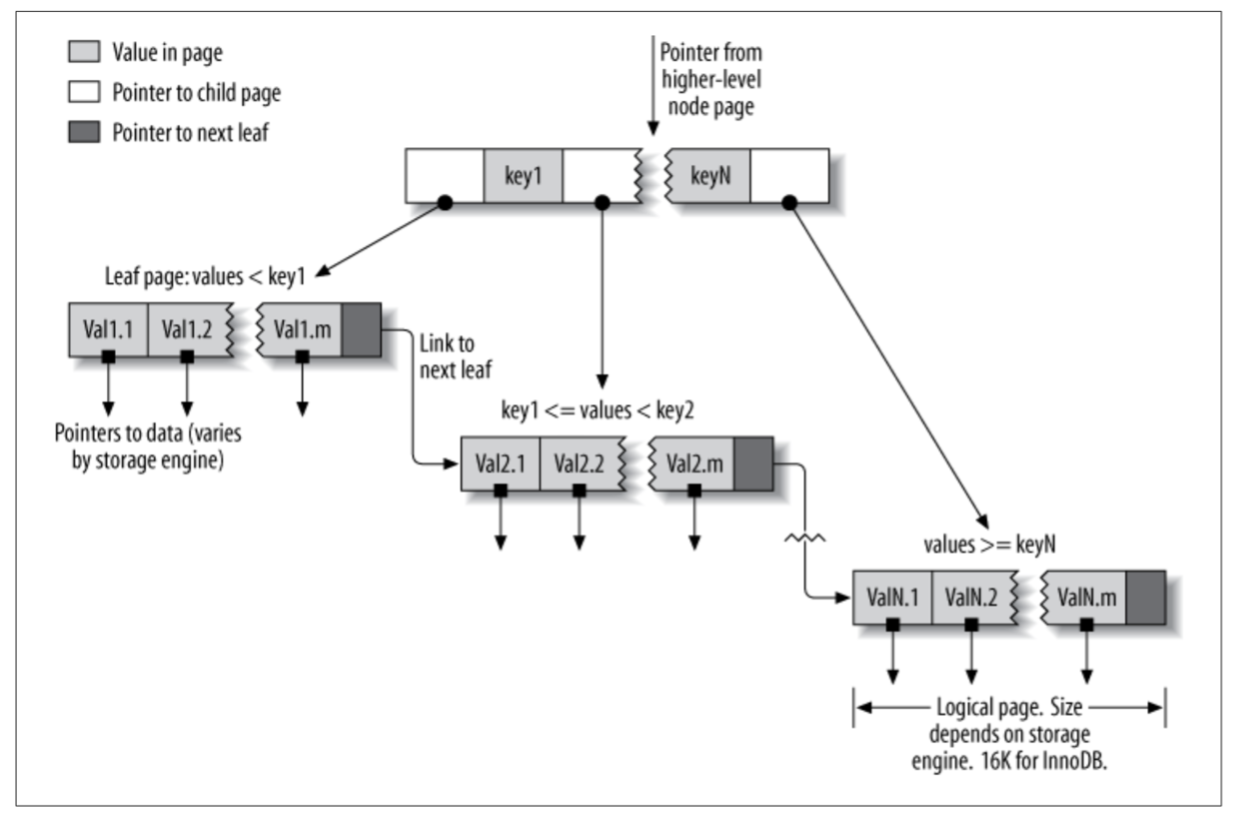
\includegraphics[width=0.65\textwidth]{PNGs/Textbook/B_Tree_Visualisation}
    \caption[Binärbaum-Visualisierung]{Binär-Baums-Darstellung (Abbildung 5--1 aus \cite[S. 149]{schwartz2012high})}
    \label{fig:b-tree-visualisation}
\end{figure}
\vspace{-20pt}

Die Blätter sind besonders, da sie Zeiger auf die indexierten Daten enthalten, anstatt auf andere Seiten zu verweisen.
Zwischen dem Wurzelknoten und den Blattseiten können viele Ebenen von Knoten-Seiten existieren.
Die Tiefe des Baumes hängt von der Größe der Tabelle ab.
Außerdem speichern B-Bäume die indexierten Spalten in einer festgelegten Reihenfolge, was sie besonders nützlich für die Suche nach Datenbereichen macht.
Beispielsweise kann ein Index auf einem Textfeld (z.B.\ vom Typ \texttt{VARCHAR}) effizient alle Namen finden, die mit „K“ beginnen, da die Werte in alphabetischer Reihenfolge gespeichert sind.

Der Index sortiert die Werte entsprechend der Reihenfolge der in der \texttt{CREATE INDEX}-Anweisung angegebenen Spalten, beispielsweise kann man wie folgt ein Index erstellen:

\vspace{-5pt}
\begin{lstlisting}[language=SQL,caption=B-Baum-Index bestehend aus mehreren Attributen,label={lst:indexing-create-combined}]
CREATE INDEX combined_index ON KUNDEN(NAME, VORNAME, GEBURTSTAG);
\end{lstlisting}
\vspace{-8pt}

Als Nächstes werden die möglichen Abfragen betrachtet, bei denen B-Baum-Indizes besonders hilfreich sind, um ein besseres Verständnis für ihre optimale Nutzung zu gewinnen.
Eine Übereinstimmung mit dem vollständigen Schlüsselwert liefert Werte für alle Spalten im Index.
Eine beispielhafte Abfrage zur Suche nach allen Einträgen mit dem Index aus~\ref{lst:indexing-create-combined} ist die Suche nach allen Kunden, die Max Mustermann heißen und am 01.01.2000 geboren wurden.
Auch Abfragen, die nur mit dem linken Präfix übereinstimmen, können von diesem Index profitieren.
So lässt sich etwa gezielt nach dem Nachnamen „Mustermann“ suchen.
Ebenso ist es möglich, nur ein Spaltenpräfix zu verwenden, etwa um alle Nachnamen zu finden, die mit „M“ beginnen.
Ein weiterer Vorteil ergibt sich bei Bereichsabfragen, denn der Index kann effizient genutzt werden, um Nachnamen zwischen „Mustermann“ und „Müller“ zu ermitteln.
Darüber hinaus unterstützt ein B-Baum-Index auch Kombinationen aus exakten und Bereichsabfragen, beispielsweise wenn nach dem Nachnamen „Mustermann“ gesucht wird, während der Vorname innerhalb eines Bereichs liegt, etwa ab „Ma“.
Ein weiterer Vorteil von B-Baum-Indizes ist, dass sie aufgrund der sortierten Baumstruktur nicht nur Abfragen, sondern auch \texttt{ORDER BY}-Bedingungen effizient unterstützen können.

Es gibt jedoch Einschränkungen von B-Baum-Indizes, die dazu führen, dass andere Indextypen für bestimmte Szenarien besser geeignet sind.
Eine Einschränkung ist, dass die Suche nicht am rechten Ende des Indexes beginnen kann.
Beispielsweise ist der Beispiels-Index nicht dazu geeignet, alle Personen zu finden, die vor dem Jahr 2000 geboren wurden, ohne dass der Nachname und Vorname ebenfalls spezifiziert werden.
Für optimale Leistung kann es auch erforderlich sein, dass Indizes mit den gleichen Spalten, jedoch in unterschiedlicher Reihenfolge erstellt werden.
Auf diese Weise könnten mehr Kombinationen abgedeckt und zusätzlich einige Abfragen optimiert werden.

Im nächsten Abschnitt werden die Benchmarks durchgeführt, um das Verständnis für die Funktionsweise des B-Baum-Index zu bestätigen.
Dazu wird zunächst wieder die Kundentabelle (\ref{lst:tools-create-table-kunde}) erstellt und für den ersten Vergleich werden folgende Indizes definiert:

\vspace{-5pt}
\begin{lstlisting}[language=SQL,caption=Definition mehrere Indizes,label={lst:indexing-create-multiple}]
CREATE INDEX idx_stadt ON KUNDEN(STADT);
CREATE INDEX idx_postleitzahl ON KUNDEN(POSTLEITZAHL);
CREATE INDEX idx_geburtstag ON KUNDEN(GEBURTSTAG);
\end{lstlisting}
\vspace{-5pt}

Um die Effizienz dieser Indizes einordnen zu können, wird diese Konfiguration mit einer verglichen, bei der nur die Kundentabelle ohne Indizes erstellt wird.
In beiden Fälle werden eine bestimmte Anzahl an Datensätze eingefügt.
Um die Performance der Select-Abfragen zu messen, werden verschiedene Queries an die Datenbank ausgeführt, bei denen die Attribute \texttt{GEBURTSTAG}, \texttt{STADT} und \texttt{POSTLEITZAHL} berücksichtigt werden.
Dazu gehören \texttt{GROUP BY}- und \texttt{COUNT}-Abfragen, bei denen die Index-Attribute verwendet werden oder sie spielen in der \texttt{WHERE}-Bedingung eine Rolle.
Damit es übersichtlich bleibt, werden einmal 10 Datensätze mit 40 und einmal 400 mit 4000 Zeilen verglichen.

\begin{figure}[H]
    \centering
    \begin{subfigure}[t]{0.48\textwidth}
        \centering
        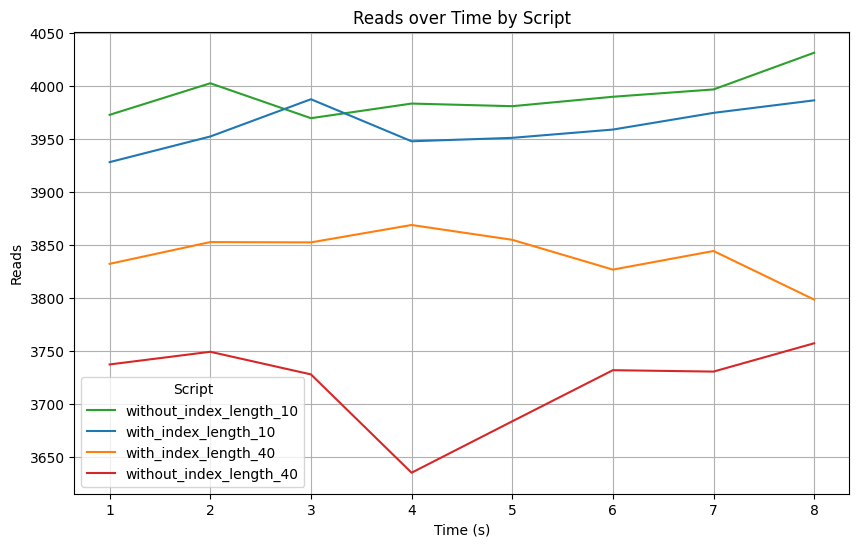
\includegraphics[width=\textwidth]{PNGs/Script/Index/B_Tree/low-count/Reads}
        \caption{Mit 10 und 40 Datensätze}
        \label{indexing-b-tree-low-reads}
    \end{subfigure}
    \hfill
    \begin{subfigure}[t]{0.48\textwidth}
        \centering
        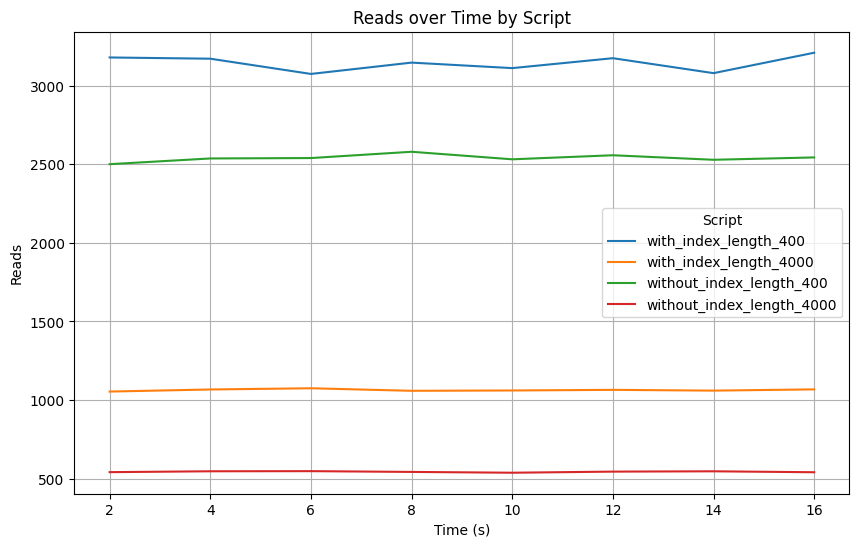
\includegraphics[width=\textwidth]{PNGs/Script/Index/B_Tree/high-count/Reads}
        \caption{Mit 400 und 4000 Zeilen}
        \label{indexing-b-tree-high-reads}
    \end{subfigure}
    \caption[B-Tree-Indexing: Mit Index vs Ohne]{Grafik zeigt Performance mit und ohne Index für Readsabfragen}
    \label{fig:indexing-vs-no}
\end{figure}
\vspace{-15pt}

In der Abbildung~\ref{indexing-b-tree-low-reads} ist zu erkennen, dass bei 10 Datensätzen die Kundentabelle ohne Indizes schneller ist als die mit Indizes.
Bei 40, 400 oder 4000 Zeilen (siehe~\ref{indexing-b-tree-high-reads}) wird schon die Wirkung der Indizes deutlich, da in diesen Fällen jeweils die Version mit Indizes effizienter ist.
Der Unterschied bei 40 Datensätzen ist zwar etwas geringer, aber in den anderen Fällen sehen noch eindeutigere Unterschiede.
Interessant ist, dass es nicht linear oder quadratisch mit der Anzahl an Datensätzen in der Tabelle steigt, sondern bei 400 und 4000 Zeilen beträgt der Unterschied zur Tabelle ohne Index jeweils etwa 500--700 Abfragen.
Bei der Schreibgeschwindigkeit liegen beide auf einem sehr ähnlichen Niveau, wobei die Version ohne Index tendenziell einen leichten Vorteil hat.

Mit dem vorherigen Benchmark können die Vorteile eines Indexes bereits deutlich erkannt werden.
Nun soll jedoch auch die Funktionalität des B-Tree-Indexes in Bezug auf unterschiedliche Selects untersucht werden.
Dazu wird erneut die Kundentabelle erstellt, aber diesmal wird nur ein Index definiert (siehe~\ref{lst:indexing-create-combined}).

Anschließend wird die Tabelle mit einer festgelegten Anzahl an Datensätzen befüllt und es werden unterschiedliche Select-Befehle ausgeführt.
Im Codeblock~\ref{lst:indexing-b-tree-selects} sind aus Platzgründen nur die Where-Bedingungen zu sehen und am Ende jeder Zeile steht der Name der Query, damit später in der Analyse nachvollzogen werden kann, welche Query welche Performance liefert.

\newpage
\begin{lstlisting}[language=SQL,caption=Unterschiedliche Where-Bedingungen für B-Tree-Index,label={lst:indexing-b-tree-selects},basicstyle=\ttfamily\scriptsize]
WHERE NAME LIKE 'M%'; -- columm_prefix
WHERE NAME = 'Müller' AND VORNAME = 'Max' AND GEBURTSTAG < '1980-01-01'; -- combined_match_with_range
WHERE NAME = 'Müller' AND VORNAME LIKE 'M%' ORDER BY GEBURTSTAG; -- exact_with_prefix
WHERE NAME = 'Müller' AND VORNAME = 'Max' AND GEBURTSTAG = '1960-01-01'; -- full_match
WHERE NAME = 'Müller'; -- leftmost_prefix
WHERE GEBURTSTAG < '1980-01-01'; -- not_leftmost
WHERE NAME BETWEEN 'Müller' AND 'Schulz'; -- range_values
WHERE NAME = 'Müller' AND VORNAME LIKE 'M%' AND GEBURTSTAG < '1980-01-01'; -- range_with_like
WHERE NAME = 'Müller' AND GEBURTSTAG < '1980-01-01'; -- skip_columns
\end{lstlisting}
\vspace{-5pt}

Anhand der Grafik in Abbildung~\ref{fig:indexing-b-tree-query-reads} lässt sich erkennen, bei welchen Abfragen der Index am effizientesten ist.
Auf der linken Seite können die Ergebnisse für die Read-Befehle mit Index betrachtet werden, während auf der rechten Seite die Werte ohne Index zu sehen sind.

\vspace{-5pt}
\begin{figure}[H]
    \centering
    \begin{subfigure}[t]{0.48\textwidth}
        \centering
        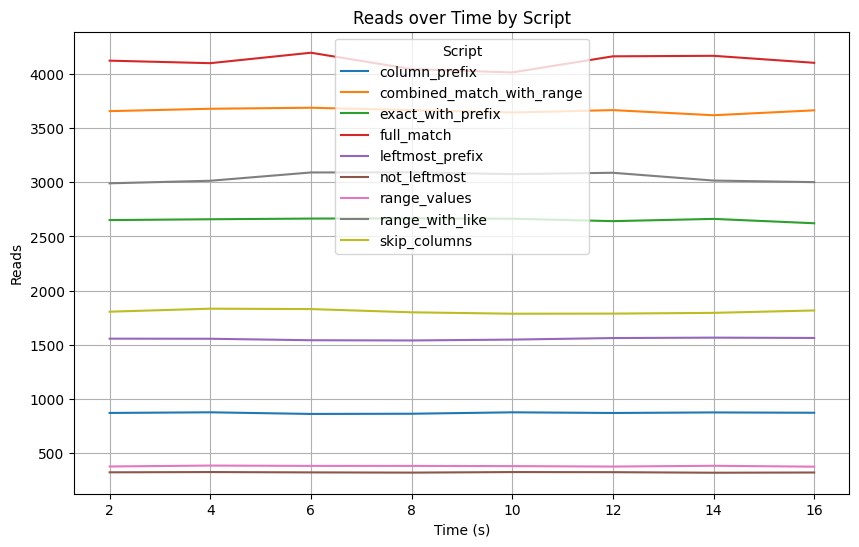
\includegraphics[width=\textwidth]{PNGs/Script/Index/B_Tree/b-tree-query-differences/Reads}
        \caption{Mit Index}
        \label{indexing-b-tree-query-reads-index}
    \end{subfigure}
    \hfill
    \begin{subfigure}[t]{0.48\textwidth}
        \centering
        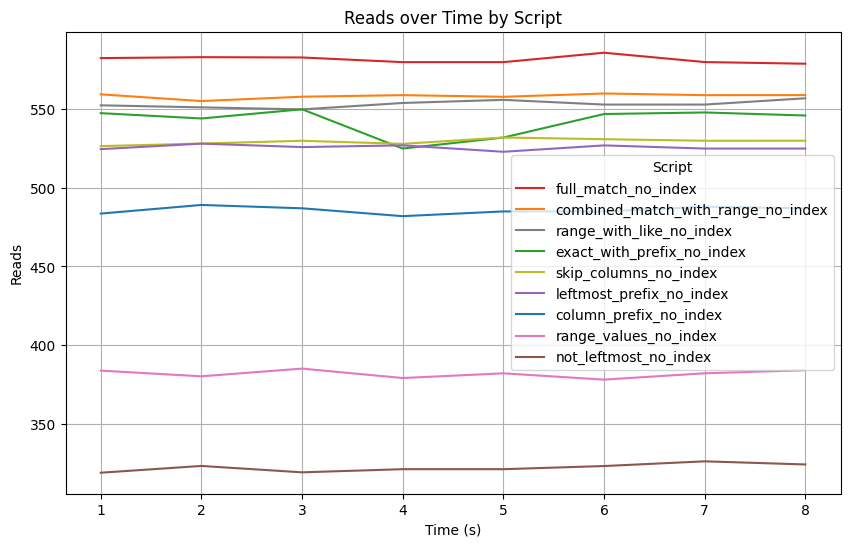
\includegraphics[width=\textwidth]{PNGs/Script/Index/B_Tree/b-tree-query-differences-no-index/Reads}
        \caption{Ohne Index}
        \label{indexing-b-tree-query-reads-no-index}
    \end{subfigure}
    \vspace{-5pt}
    \caption[B-Tree-Indexing: Unterschiedliche Selects mit Index und Ohne]{Visualisierung von unterschiedlichen Select-Queries mit und ohne Index}
    \label{fig:indexing-b-tree-query-reads}
\end{figure}
\vspace{-15pt}

Zunächst fällt auf, dass die Reihenfolge für die Werte mit und ohne Index komplett identisch ist.
Dies ist direkt erkennbar, da die Legenden beider Grafiken nach dem durchschnittlichen Wert über die gesamte Zeit sortiert sind.
Damit die richtigen Schlüsse aus der Grafik gezogen werden können, muss zunächst ermittelt werden, wie viele Zeilen die unterschiedlichen Queries zurückgeben.
Dazu werden die Abfragen zusätzlich mit dem \texttt{COUNT(*)}-Operator durchgeführt und die Ergebnisse in die Log-Datei geschrieben.
Anschließend werden die Werte entnommen und in einer Tabelle zusammengefasst.

\vspace{-5pt}
\begin{table}[H]
    \centering
    \scriptsize
    \begin{tabular}{|l|l|l|l|}
        \hline
        \textbf{Select-Query} & \textbf{Anzahl an Zeilen} & \textbf{Faktor} & \textbf{Index benutzt?} \\
        \hline
        full\_match & 0 & 6.42 & ja \\
        combined\_match\_with\_range & 13 & 5.78 & ja \\
        range\_with\_like & 31 & 5.22 & ja \\
        exact\_with\_prefix & 51 & 5.14 & ja \\
        skip\_columns & 147 & 3.47 & ja \\
        leftmost\_prefix & 263 & 2.73 & ja \\
        column\_prefix & 551 & 1.69 & ja \\
        range\_values & 1343 & 0.96 & nein \\
        not\_leftmost & 2371 & 0.98 & nein \\
        \hline
    \end{tabular}
    \vspace{3pt}
    \caption{Ergebnisse der COUNT(*)-Abfragen für B-Tree-Index}
    \label{tab:indexing_b_tree_count_results}
\end{table}
\vspace{-25pt}

Anhand der Spalte \texttt{Anzahl an Zeilen} lässt sich erkennen, dass die Queries, die am wenigsten Zeilen zurückgeben, auch diejenigen sind, bei denen die höchste Performance erzielt wird.
Deshalb ist auch die Reihenfolge mit und ohne Index gleich, weshalb man meinen könnte, dass der Index keinen Einfluss auf die Performance hat.
Dies betrifft jedoch nur die Reihenfolge, nicht aber die Werte der Abfragen, da hier deutliche Unterschiede erkennbar sind.
Anschaulich wird das mit der Betrachtung der Spalte \texttt{Faktor}.
Um den Wert zu berechnen, werden die Werte aus der Gesamtstatistik entnommen und die Version mit Index durch die Version ohne Index geteilt.
Dadurch lässt sich erkennen, dass \texttt{full\_match} zwar bei beiden Versionen am schnellsten ist, jedoch mit Index etwa 6-mal schneller als ohne.
Es lässt sich auch erkennen, dass je weniger Zeilen zurückgegeben werden, desto größer ist der Faktor.
Bei den Queries \texttt{range\_values} und \texttt{not\_leftmost} liegt der Faktor sehr nah 1, was bedeutet, dass der Index keinen Einfluss auf die Performance hat.
Deshalb stellt sich auch die Frage, ob der Index überhaupt verwendet wird.
Um das zu überprüfen, wird der \texttt{EXPLAIN}-Operator verwendet, das Ergebnis erneut geloggt und der Tabelle hinzugefügt (siehe Spalte \texttt{Index benutzt?}).
Und tatsächlich sehen wir, dass die vermuteten Queries die einzigen sind, bei denen der Index nicht verwendet wird.

\section{Hash-Index}\label{sec:indexing-hash-index}
Ein weiterer Indextyp, der betrachtet wird, ist der Hash-Index.
Dieser basiert auf einer Hash-Tabelle und ist daher nur für exakte Suchanfragen geeignet, die alle Spalten des Indexes verwenden.
In MySQL unterstützt nur die Memory-Storage-Engine explizite Hash-Indizes.
Einige Storage-Engines, wie zum Beispiel InnoDB, können erkennen, wenn bestimmte Index-Werte besonders häufig abgefragt werden.
Sie erstellen dann automatisch einen Hash-Index für diese Werte im Speicher, der zusätzlich zu den bestehenden B-Baum-Indizes genutzt wird.
Die Funktionsweise der Storage-Engine lässt sich wie folgt beschreiben.

Für jede Zeile wird mithilfe einer Hash-Funktion ein Hash-Wert der indexierten Spalte berechnet.
Der Hash-Wert (engl.\ hash code) ist eine kleine Zahl, die sich in der Regel von den Hash-Werten anderer Zeilen mit unterschiedlichen Schlüsselwerten unterscheidet.
Anschließend wird die Position im Index gesucht und man findet einen Zeiger auf die entsprechende Zeile.
In letzten Schritt überprüft man die Werte der Zeile, um sicherzustellen, dass es sich um die richtige Zeile handelt.

Wenn mehrere Werte denselben Hash-Wert besitzen, speichert der Index die Zeiger auf die Zeilen (engl.\ row pointers) in demselben Hash-Tabelleneintrag, typischerweise mithilfe einer verketteten Liste (z.B.\ einer \textit{Linked List}).
Hash-Kollisionen können die Leistung eines Hash-Index beeinträchtigen, da jeder Zeiger in der verketteten Liste durchlaufen und die entsprechenden Werte mit dem Suchwert verglichen werden müssen, um die richtigen Zeilen zu finden.
Das ist auch Index-Wartungsoperationen mit viel Aufwand verbunden.
Hingegen eindeutige Hash-Indizes stellen sicher, dass für jeden Hash-Wert nur ein einziger Eintrag existiert.
Bei Konflikten wird ein Mechanismus wie die Open Addressing-Strategie (z.B.\ Linear Probing oder Quadratic Probing) eingesetzt, um Konflikte zu lösen und den Speicherplatz effizient zu verwalten.
Hierbei wird versucht, Konflikte direkt innerhalb der Hash-Tabelle zu bewältigen, anstatt auf zusätzliche Datenstrukturen wie verkettete Listen zurückzugreifen.
Die eindeutigen Hash-Indizes werden nicht von der Memory-Engine in MySQL unterstützt.

Um die Verwendung des Hash-Indexes zu veranschaulichen, benutzen folgt folgendes Beispiel:

\vspace{-5pt}
\begin{lstlisting}[language=SQL]
SELECT * FROM KUNDEN WHERE NAME = 'Peter';
\end{lstlisting}
\vspace{-8pt}

Zunächst berechnet MySQL den Hash-Wert für \texttt{'Peter'} und verwendet diesen, um den entsprechenden Zeiger im Index zu finden.
Angenommen, die Hash-Funktion liefert für \texttt{'Peter'} den Wert \textbf{7654}.
MySQL sucht nun im Index an der Position 7654 und findet einen Zeiger auf Zeile 3.
Im letzten Schritt wird der Wert in Zeile 3 mit \texttt{'Peter'} verglichen.
Da die Indizes nur kompakte Hash-Werte speichern, sind Hash-Indizes äußerst platzsparend und Suchvorgänge erfolgen in hoher Geschwindigkeit.

Ähnlich wie der B-Baum-Index hat auch der Hash-Index einige Einschränkungen.
Zum einen enthält der Index nur Hash-Werte und Zeiger auf Zeilen (engl.\ row pointers), jedoch nicht die Werte selbst.
Deshalb kann MySQL den Index nicht verwenden, um das Einlesen der Zeilen zu vermeiden.
Allerdings erfolgt der Zugriff auf die in den Speicher geladenen Zeilen sehr schnell, wodurch die Leistung nicht wesentlich beeinträchtigt ist.
Zum anderen können Hash-Indizes nicht für Sortierungen verwendet werden, da die Werte nicht in einer geordneten Reihenfolge gespeichert sind.
Im Gegensatz dazu sind B-Baum-Indizes in der Lage.
Darüber hinaus ermöglichen Hash-Indizes keine partiellen Schlüsselübereinstimmungen (engl.\ partial key matching).
Da der Hash-Wert aus dem gesamten indexierten Wert berechnet wird, hilft ein Hash-Index beispielsweise nicht, wenn ein Index aus den Spalten (A, B) besteht und die \texttt{WHERE}-Klausel nur auf A verweist.
Ein weiterer Nachteil besteht darin, dass Hash-Indizes keine Bereichsabfragen unterstützen.
Sie eignen sich lediglich für Gleichheitsvergleiche, wie die Operatoren \texttt{=} (gleich), \texttt{<=>} (null-sicher gleich) und \texttt{IN()}.

Als Nächstes werden die Benchmarks mit Hash-Indizes betrachtet.
Dazu wird erneut die Kundentabelle verwendet und diesmal nur ein Index für die Spalte \texttt{NAME} erstellt.
Am Ende des \texttt{CREATE INDEX}-Befehls muss \texttt{USING HASH} hinzugefügt werden, damit statt des standardmäßigen B-Tree-Index der Hash-Index verwendet wird.
Danach befüllen wieder die Tabelle mit Testdaten.
Diesmal wird beim ersten Benchmark der Einfluss von Hash-Kollisionen auf die Performance untersucht.
Um den Grad der Kollisionen zu verändern, wird eine Variable verwendet, die die obere Grenze für die zufällige Generierung einer Zahl darstellt.
Anschließend werden alle Zeilen mit dem Wert \texttt{Kunde\_1} für die Spalte \texttt{NAME} abgefragt und die Tests werden mit den Kollisionswahrscheinlichkeiten von 25\%, 10\%, 5\% und 1\% durchgeführt.

\vspace{-4pt}
\begin{figure}[H]
    \centering
    \begin{subfigure}[t]{0.48\textwidth}
        \centering
        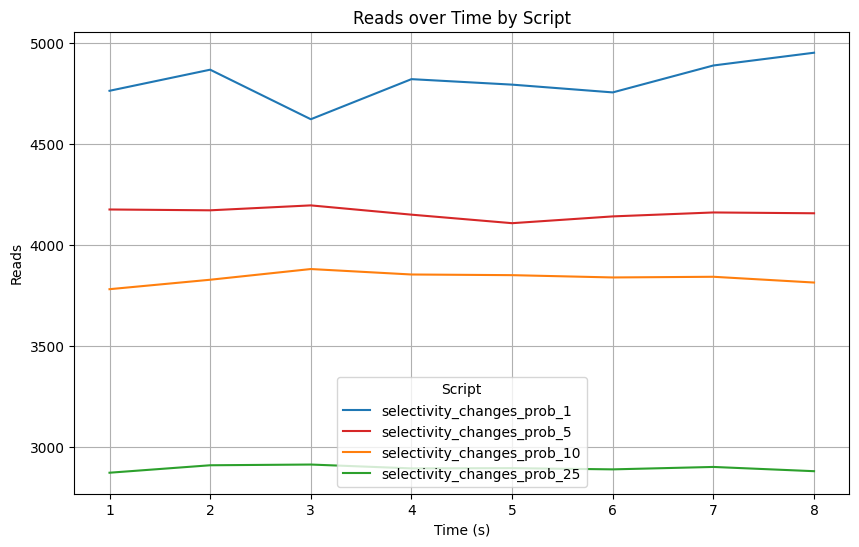
\includegraphics[width=\textwidth]{PNGs/Script/Index/Hash/hash-selectivity-change/Reads}
    \end{subfigure}
    \hfill
    \begin{subfigure}[t]{0.48\textwidth}
        \centering
        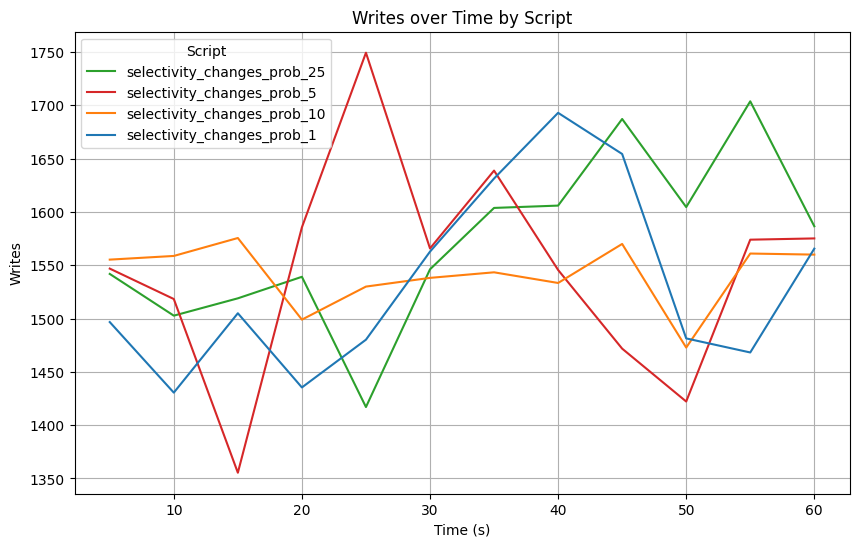
\includegraphics[width=\textwidth]{PNGs/Script/Index/Hash/hash-selectivity-change/Writes}
    \end{subfigure}
    \vspace{-8pt}
    \caption[Hash-Indexing: Auswirkungen von Hashkollisionen]{Vergleich der Auswirkungen von Hashkollisionen}
    \label{fig:hash-collision-comparison}
\end{figure}
\vspace{-17pt}

An den Ergebnissen in Abbildung~\ref{fig:hash-collision-comparison} ist zu erkennen, dass je geringer die Wahrscheinlichkeit für eine Kollision ist, desto schneller fällt die Select-Abfrage aus.
Es fällt auch auf, dass die Unterschiede zwischen den verschiedenen Kollisionswahrscheinlichkeiten sehr groß sind.
Hingegen die Einfüge-Performance ist bei allen 4 Varianten auf einem ähnlichen Niveau.

Als zweiten Test soll überprüft werden, ob der Index bei bestimmten Select-Queries benutzt wird oder nicht.
Dazu wird erneut die Kundentabelle verwendet, der gleiche Index wie in Beispiel~\ref{lst:indexing-create-combined} erstellt, die Testdaten eingefügt und die Select-Befehle aus~\ref{lst:indexing-b-tree-selects} genutzt.
Dieses Mal werden aber nicht alle Select-Befehle verwendet, sondern nur die aus folgender Tabelle:

\vspace{-4pt}
\begin{table}[H]
    \centering
    \scriptsize
    \begin{tabular}{|l|l|l|l|}
        \hline
        \textbf{Select-Query} & \textbf{Anzahl an Zeilen} & \textbf{Faktor} & \textbf{Index benutzt?} \\
        \hline
        full\_match & 0 & 2.67 & ja \\
        combined\_match\_with\_range & 6 & 0.97 & nein \\
        exact\_with\_prefix & 45 & 1.01 & nein \\
        leftmost\_prefix & 206 & 1.00 & nein \\
        \hline
    \end{tabular}
    \vspace{3pt}
    \caption{Ergebnisse der COUNT(*)-Abfragen für Hash-Index}
    \label{tab:indexing_hash_count_results}
\end{table}
\vspace{-30pt}

Anhand der Spalten \texttt{Faktor} und \texttt{Index benutzt?} kann erkannt werden, dass der Index nur bei der \texttt{full\_match}-Abfrage benutzt wird.
Das stimmt auch mit den Ergebnissen aus der Abbildung~\ref{fig:indexing-hash-query-reads} überein, da ohne Index alle Abfragen auch einem ähnlichen Niveau liegen, aber mit Index sticht eine deutlich hervor.
Interessant ist, dass die Query mit 206 zurückgegebenen Zeilen nur unwesentlich langsamer ist als die anderen.
Die Reihenfolge ist wieder bei beiden identisch und hängt von der Anzahl der zurückgegebenen Zeilen ab.

\vspace{-4pt}
\begin{figure}[H]
    \centering
    \begin{subfigure}[t]{0.48\textwidth}
        \centering
        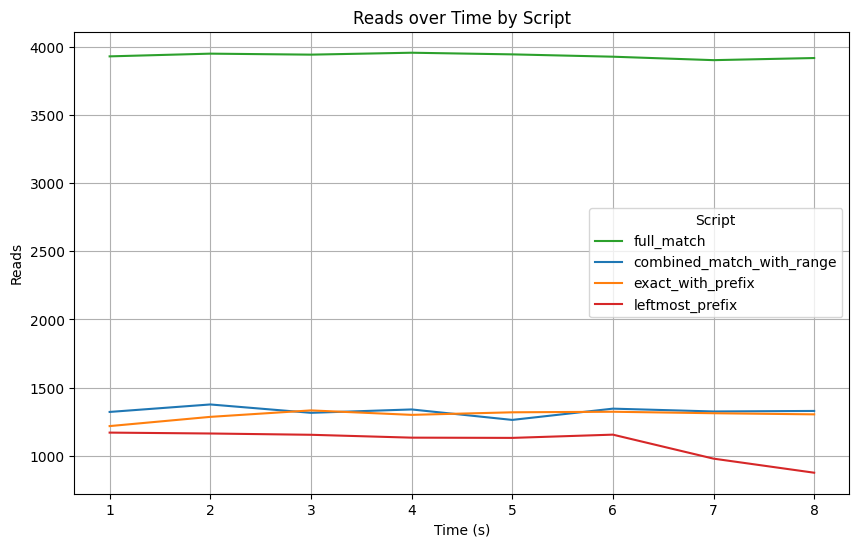
\includegraphics[width=\textwidth]{PNGs/Script/Index/Hash/hash-query-differences/Reads}
    \end{subfigure}
    \hfill
    \begin{subfigure}[t]{0.48\textwidth}
        \centering
        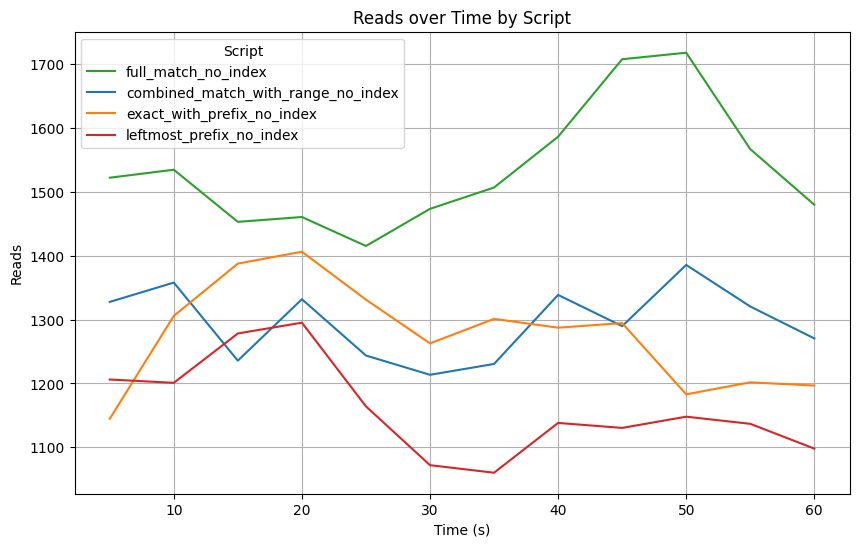
\includegraphics[width=\textwidth]{PNGs/Script/Index/Hash/hash-query-differences-no-index/Reads}
    \end{subfigure}
    \vspace{-8pt}
    \caption[Hash-Indexing: Unterschiedliche Abfragen mit Index und Ohne]{Grafik visualisiert Select-Queries mit (links) und ohne (rechts) Index}
    \label{fig:indexing-hash-query-reads}
\end{figure}

\section{Vergleich von B-Tree- und Hash-Index}\label{sec:indexing-comp-b-tree-hash-index}

In den vorherigen Kapiteln wurden der B-Tree-Index und der Hash-Index jeweils getrennt voneinander betrachtet.
Dabei wurde auch analysiert, bei welchen Select-Queries die Indizes Vorteile bieten und bei welchen nicht.
Damit fehlt uns noch der Vergleich zwischen dem B-Tree-Index und dem Hash-Index.

Um die Unterschiede zwischen beiden Indexstrukturen genauer zu analysieren, wird ein neuer Benchmark durchgeführt, der die Skripte aus Kapitel~\ref{sec:indexing-b-baum-index} und~\ref{sec:indexing-hash-index} wiederverwendet.
Da der Hash-Index aber nur 4 unterschiedliche Select-Queries aufruft, sollen auch nur diese mit dem B-Tree-Index ausgeführt werden.
Dazu wird einfach der Parameter~\texttt{selects} beim Aufruf des Orchestrator-Skripts hinzugefügt und das Skript anschließend ausgeführt.

\vspace{-4pt}
\begin{figure}[H]
    \centering
    \begin{subfigure}[t]{0.48\textwidth}
        \centering
        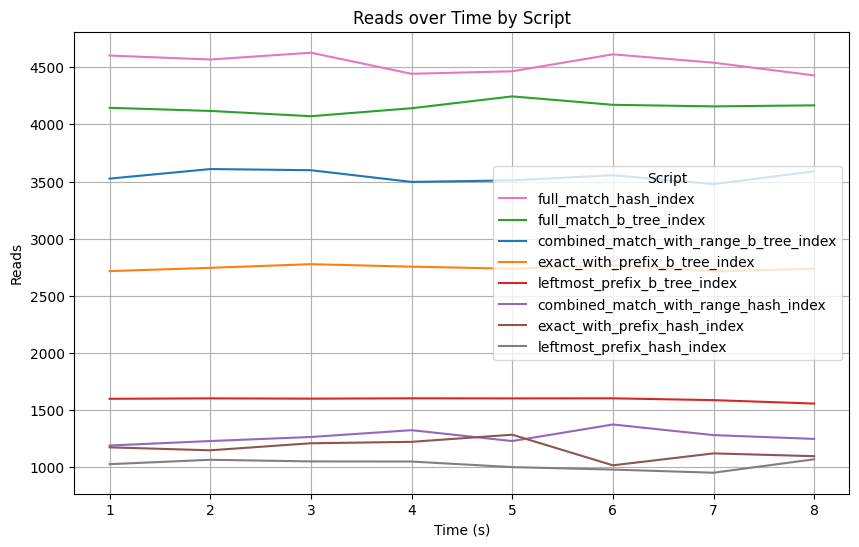
\includegraphics[width=\textwidth]{PNGs/Script/Index/B_Tree/hash-vs-b-tree-comparison/Reads}
        \caption{Anzahl der Lesezugriffe}
        \label{indexing-hash-vs-b-tree-comparison-reads}
    \end{subfigure}
    \hfill
    \begin{subfigure}[t]{0.48\textwidth}
        \centering
        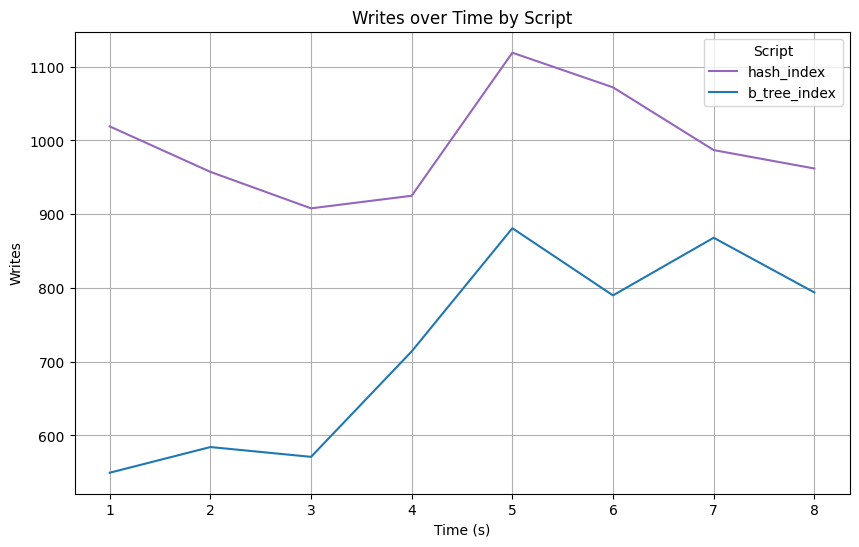
\includegraphics[width=\textwidth]{PNGs/Script/Index/B_Tree/hash-vs-b-tree-comparison/Writes}
        \caption{Anzahl der Schreibzugriffe}
        \label{indexing-hash-vs-b-tree-comparison-writes}
    \end{subfigure}
    \vspace{-2pt}
    \caption[Indexing: Vergleich von B-Tree- und Hash-Index]{Vergleich der Select-Query-Performance von B-Tree- und Hash-Index}
    \label{fig:indexing-hash-b-tree-comp}
\end{figure}
\vspace{-12pt}

In der Abbildung~\ref{indexing-hash-vs-b-tree-comparison-reads} sehen die Performance für die unterschiedlichen Select-Befehle.
Die höchste Transaktionsrate erzielt der Hash-Index, sofern der vollständige Schlüssel angegeben wird (\texttt{full\_match}).
Dicht darauf folgt der B-Tree-Index mit derselben Abfrage, allerdings mit etwa 10\% weniger Zugriffen.
Bei den übrigen Abfragen schneidet hingegen der B-Tree-Index deutlich besser ab, in einigen Fällen sogar bis zu dreimal schneller als der Hash-Index.
Der Grund dafür ist bereits aus den anderen Kapiteln bekannt.
Da der Hash-Index nur bei exaktem Schlüsselabgleich zum Einsatz kommt, wird er bei den anderen Abfragen nicht verwendet.
Mithilfe des \texttt{EXPLAIN}-Operators wurde festgestellt, dass stattdessen der B-Tree-Index verwendet wird, was die starken Unterschiede erklärt.

Betrachtet man die Schreibperformance (Abbildung~\ref{indexing-hash-vs-b-tree-comparison-writes}), zeigt sich, dass der Hash-Index etwa 30--40\% schneller ist als der B-Tree-Index.
Wenn eine Anwendung also eine hohe Schreiblast hat, könnte der Hash-Index eine bessere Wahl sein, da er weniger Mehraufwand verursacht.
Zusammenfassend lässt sich festhalten, dass der Hash-Index einen leichten Vorteil hat, wenn beide Indexe greifen.
Andernfalls überwiegen die Stärken des B-Tree-Indexes.

%! Author = danielmendes
%! Date = 26.01.25

\chapter{Views}\label{ch:views}
Im folgenden Kapitel werden die Performancevorteile von Sichten (engl.\ Views) in SQL betrachtet.
Zunächst wird auf virtuelle Sichten, ihre Vor- und Nachteile, das Verhalten bei Inserts sowie auf mögliche Szenarien eingegangen, in denen sie besonders vorteilhaft sein können.
Anschließend wird sich mit materialisierten Sichten beschäftigt, die physisch in der Datenbank gespeichert werden.
Zunächst wird eine Version mit Triggern implementiert, da MySQL keine native Unterstützung für materialisierte Sichten bietet, bevor die native Implementierung in PostgreSQL genutzt wird.
In den letzten beiden Kapiteln wird die Durchführung der Benchmarks näher betrachtet und die entstandenen Ergebnisse interpretiert.

\section{Virtuelle Views}\label{sec:virtuelle-views}

Grundlegend existieren Relationen, bzw.\ Tabellen, die durch das \texttt{CREATE TABLE}-Statement definiert werden, physisch in der Datenbank.
Damit sind sie persistent, was bedeutet, dass sie dauerhaft existieren und sich nicht ändern, es sei denn, sie werden explizit durch eine SQL-Änderungsanweisung dazu aufgefordert.
Dies entspricht der Dauerhaftigkeit des ACID-Prinzips (\cite[S. 630--631]{silberschatz2011database}), die sicherstellt, dass bestätigte Transaktionen dauerhaft gespeichert bleiben und auch bei Systemausfällen nicht verloren gehen.
Es gibt jedoch eine weitere Klasse von SQL-Relationen, die nicht wie Tabellen physisch gespeichert werden (\cite[341--349, 353--366]{garcia2008database}).
%~\cite[S. 276--281]{schwartz2012high}
Sie werden als virtuelle Sichten bezeichnet.

\begin{quote}
    \enquote{A view is a table whose rows are not explicitly stored in the database but are computed as needed from a view definition.} (\cite[S. 86]{ramakrishnan2002database})
\end{quote}

Virtuelle Sichten werden durch einen Ausdruck definiert, der einer Abfrage ähnelt.
Sie können auch so abgefragt werden, als ob sie tatsächlich physisch existierten (vgl.\ \cite[S. 87]{ramakrishnan2002database}).
In einigen Fällen lassen sich sogar Datensätze über die Sicht ändern.

\vspace{-5pt}
\begin{lstlisting}[language=SQL,caption=Allgemeine View-Deklaration,label={lst:create_view}]
CREATE VIEW <name> AS <view-definition>;
\end{lstlisting}
\vspace{-5pt}

In dem Codeblock~\ref{lst:create_view} wird die Struktur der Definition einer View gezeigt.
Als Nächstes muss die \texttt{view-definition} mit einer SQL-Abfrage ersetzt werden, die den Inhalt der virtuellen Sicht abbilden soll.
Um dieses Vorgehen mit einem Beispiel näher zu veranschaulichen, werden die Tabellen Kunden (\ref{lst:tools-create-table-kunde}) und Bestellung (\ref{lst:tools-create-table-bestellung}) genutzt.
Nun wollen wir, dass die beiden Tabellen über die \texttt{KUNDEN\_ID} in der Sicht zusammengefügt werden, da sie sowohl der Primärschlüssel in der Kundentabelle als auch der Fremdschlüssel in der Bestellung ist.
Um in die SQL-Abfrage noch etwas mehr Komplexität zu bringen, soll neben der Join-Operation auch der Umsatz pro Jahr und pro Stadt aggregiert werden.
Die View \texttt{KUNDEN\_OVERVIEW} hat folgende Struktur:

\vspace{-5pt}
\lstinputlisting[
    language=sql,
    caption=View Deklarierung,
    label={lst:create_kunden_bestellung_view},
    style=custom_daniel,
]{Scripts/Views/01_create_view.sql}

Diese Aggregation könnte beispielsweise von einem Marketingteam genutzt werden, um schwache Regionen pro Jahr zu identifizieren und gezielt in diesen nachzusteuern.
Wenn die Daten dieser virtuellen Sicht abgefragt werden sollen, wird der Name in der FROM-Klausel adressiert und es wird darauf vertraut, dass das Datenbankmanagementsystem die benötigten Tupel erzielt (siehe~\ref{lst:select-view}).
Dabei operiert das DBMS direkt auf den Relationen, die die virtuelle Sicht definieren.
In diesem Fall handelt es sich um die Kunden- und Bestelltabelle.

\vspace{-5pt}
\begin{lstlisting}[language=SQL,caption=SQL-Befehl mit verwendeter View,label={lst:select-view}]
SELECT * FROM KUNDEN_OVERVIEW
ORDER BY Jahr ASC, Gesamtumsatz DESC;
\end{lstlisting}
\vspace{-5pt}

Eine weitere Möglichkeit, die Funktionsweise einer Sicht besser zu verstehen, besteht darin, sie in einer FROM-Klausel durch eine Unterabfrage zu ersetzen, die identisch mit der Sichtdefinition ist.
Damit Bezug auf die Tupel genommen werden kann, muss die Unterabfrage noch mit einer Tupelvariablen ergänzt werden.
Die SQL-Abfrage aus~\ref{lst:select-without-view} liefert das gleiche Ergebnis wie die aus~\ref{lst:select-view}, wenn die View wie im Beispiel~\ref{lst:create_kunden_bestellung_view} definiert wird.
Zu dem Einfluss auf die Performance wird im Unterkapitel~\ref{sec:durchfuhrung-der-benchmarks} eingegangen.

\lstinputlisting[
    language=sql,
    caption=Select-Befehl ohne Sicht,
    label={lst:select-without-view},
    style=custom_daniel,
]{Scripts/Views/02_select_without_view.sql}

Man kann den Attributen einer Sicht auch eigene Namen vergeben, indem man sie in Klammern hinter dem Namen der Sicht aus der \texttt{CREATE VIEW}-Anweisung auflistet.
Die Definition einer Sicht kann mit \texttt{DROP VIEW <view-name>} gelöscht werden, wodurch keine Abfragen mehr auf dieser Sicht ausgeführt werden können.
Das Löschen der Sicht hat jedoch keine Auswirkungen auf die Tupel der zugrundeliegenden Tabellen.
Im Gegensatz dazu würde \texttt{DROP TABLE <table-name>} die Tabelle löschen und damit auch die darauf basierenden Sichten unbrauchbar machen, da ihre Definitionen auf der gelöschten Tabelle beruhen.

Abgesehen vom Löschen der Tabellen kann man auch Einfügungen an der View durchführen.
Dies ist aber nicht uneingeschränkt möglich und nur unter bestimmten Bedingungen erlaubt.
Zum einen muss die Sicht durch eine einfache Abfrage aus nur einer einzigen Relation definiert sein.
Zum anderen muss die \texttt{SELECT}-Klausel ausreichend Attribute umfassen, sodass fehlende Werte bei Einfügungen mit \texttt{NULL} oder anderen definierten Standardwerten ergänzt werden können.
Die Änderungen werden dann direkt auf die Basistabelle angewendet, wobei nur die in der Sicht definierten Attribute berücksichtigt werden.
Wenn die eben beschriebenen Bedingungen erfüllt sind, werden auch bei Löschungen und Aktualisierungen die Änderungen auf die zugrundeliegende Relation R übertragen.
Dabei wird die \texttt{WHERE}-Bedingung der View zu den Bedingungen der Änderung im \texttt{WHERE}-Block hinzugefügt.
Wenn die Bedingungen nicht erfüllt sind, wie im Beispiel (\ref{lst:create_kunden_bestellung_view}), weil mehrere Relationen in der View verwendet werden, müssen Änderungen direkt an den zugrunde liegenden Tabellen vorgenommen werden.
In diesem Fall kann die View nur für Select-Abfragen genutzt werden.

Das Einfügen über die Sicht ist jedoch nicht die intuitivste Möglichkeit, um Änderungen an den unterliegenden Tabellen durchzuführen.
Das liegt vor allem an dem Umgang mit den nicht definierten Werten, weshalb sich das Konzept von Triggern anbietet.
Trigger in SQL sind Datenbankobjekte, die mit einer Tabelle verknüpft sind und sobald bestimmte Ereignisse eintreten, führen sie eine Reihe von Anweisungen aus (vgl.\ \cite[S. 180]{silberschatz2011database}).
Die Auslösung eines Triggers kann entweder vor (\texttt{BEFORE}) oder nach (\texttt{AFTER}) einem bestimmten Ereignis erfolgen, wie \texttt{INSERT}, \texttt{UPDATE} oder \texttt{DELETE}.
Bei Triggern auf Sichten können auch \texttt{INSTEAD-OF}-Trigger verwendet werden, die Änderungsversuche an der Sicht abfangen und stattdessen eine frei definierbare Aktion ausführen.

\vspace{-5pt}
\begin{lstlisting}[language=SQL,caption=Allgemeine Trigger Deklaration,label={lst:allg-trigger-dekl}]
CREATE TRIGGER trigger_name
{BEFORE | AFTER | INSTEAD OF} {INSERT | UPDATE | DELETE}
ON {table_name | view_name}
FOR EACH ROW
trigger_body;
\end{lstlisting}
\vspace{-5pt}

Das Problem in MySQL mit Triggern ist aber, dass sie nur auf Tabellen angewendet werden können.
Später wird dazu im Kapitel~\ref{sec:durchfuhrung-der-benchmarks} noch ein genaueres Beispiel betrachtet.
Um Werte in eine virtuelle Sicht einzufügen, bietet sich jedoch das Konzept der Stored Procedures an.
Stored Procedures sind Funktionen, die direkt im DB-Server hinterlegt werden und wie andere integrierte Funktionen, wie z.B.\ round(), aufgerufen werden können.
Sie ermöglichen es, geschäftslogische Prozesse in der Datenbank zu speichern und direkt über SQL-Anweisungen auszuführen (vgl.\ \cite[S. 173]{silberschatz2011database}).

\vspace{-5pt}
\begin{lstlisting}[language=SQL,caption=Allgemeine Prozedur Deklaration,label={lst:allg-stored-procedure-dekl}]
CREATE PROCEDURE stored_procedure_name(IN param1 INT, IN param2 VARCHAR(255))
BEGIN
    -- smth
END
\end{lstlisting}
\vspace{-5pt}

Damit für die Sicht aus dem Beispiel~\ref{lst:create_kunden_bestellung_view} Daten eingefügt werden können, muss die Prozedur die gleichen Parameter wie die Spalten der View erhalten.
Die Parameter werden in der Funktion verarbeitet und die ermittelten Daten in die zugrunde liegenden Tabellen eingefügt.
Wenn die Prozedur korrekt ist, dann werden die Änderungen bei der nächsten \texttt{SELECT}-Abfrage der View sichtbar.

\vspace{-5pt}
\lstinputlisting[
    language=sql,
    caption=Deklaration der Prozedur,
    label={lst:create_trigger},
    style=custom_daniel,
]{Scripts/Views/03_create_procedure.sql}

Jetzt kann die Methode \texttt{insert\_view} einfach mit dem \texttt{CALL}-Befehl aufgerufen werden und die Werte für die drei Parameter werden in Klammern übergeben.
Dadurch werden die Werte in die Bestelltabelle eingefügt.
Als Bestelldatum wird stets der erste Tag des Jahres verwendet und als Kunde wird einer gewählt, der in dem jeweiligen Land lebt.

Im Vergleich zum direkten Einfügen in die Bestelltabelle geht jedoch Datenpräzision verloren.
Einerseits fehlt das genaue Datum und andererseits sind die Informationen zur \texttt{KUNDEN\_ID} und \texttt{ARTIKEL\_ID} nicht vorhanden.
Zusammengefasst lässt sich sagen, dass je nach Definition der Sicht Daten entweder direkt eingefügt oder mithilfe von Stored Procedures befüllt werden können.
Es ist dabei jedoch nicht ausgeschlossen, dass es in den zugrunde liegenden Tabellen zu einer geringeren Datenqualität kommen kann, da beispielsweise NULL-Werte oder andere Standardwerte verwendet werden.
Deshalb sollten virtuelle Sichten grundsätzlich nur zur Abfrage von Daten benutzt werden und nicht für Änderungen.
Stattdessen sollten die zugrunde liegenden Tabellen direkt angepasst werden.

\section{Materialisierte Views}\label{sec:materialisierte-views}

Allgemein werden Sichten so definiert, dass sie eine neue Relation aus den Basistabellen erzeugen, indem sie eine Abfrage auf diese Tabellen ausführen.
Bisher wurden Sichten ausschließlich als logische Beschreibungen von Relationen betrachtet.
In bestimmten Fällen kann es jedoch aus Performancegründen sinnvoll sein, sie zu materialisieren, also die Ergebnisse physisch zu speichern.

\begin{quote}
    \enquote{Materialized views constitute redundant data, in that their contents can be inferred from the view definition and the rest of the database contents.} (\cite[S. 607]{silberschatz2011database})
\end{quote}

Durch die physische Speicherung verringert sich der Rechenaufwand für Abfragen, da für das Beispiel (siehe~\ref{lst:create_kunden_bestellung_view}) der Join nicht erneut ausgeführt werden muss.
Die bereits gespeicherten Ergebnisse sind damit direkt abrufbar, was zu einer schnelleren Antwortzeit der Query führt.
Passend zu der virtuellen Sicht (\ref{lst:create_kunden_bestellung_view}) sieht die Materialisierte wie folgt aus:

\vspace{-5pt}
\lstinputlisting[
    language=sql,
    caption=Materialized View,
    label={lst:create_mat_view},
    style=custom_daniel,
]{Scripts/Views/04_create_mat_view.sql}

Wie zu sehen ist, unterscheidet sich die materialisierte Sicht nur in der ersten Zeile von der Virtuellen.
Einen Nachteil der materialisierten Sicht gegenüber der Virtuellen ist der zusätzliche Aufwand, ähnlich wie bei Indizes.
Wenn Änderungen an der zugrunde liegenden Basistabelle vorgenommen werden, ist die materialisierte Sicht nicht mehr aktuell.
Die einfachste Lösung besteht darin, bei jeder Änderung eine vollständige Neuberechnung der Sicht durchzuführen (vgl.\ \cite[S. 608]{silberschatz2011database}).
Dies kann explizit mit dem folgenden Befehl durchgeführt werden:

\vspace{-5pt}
\begin{lstlisting}[language=SQL,caption=Aktualisierung der materialisierten Sicht,label={lst:refresh-materialized-view}]
REFRESH MATERIALIZED VIEW KUNDEN_MAT_OVERVIEW;
\end{lstlisting}
\vspace{-5pt}

Die Anzahl an Neuberechnungen hat einen großen Einfluss auf die Performance, weshalb man sich ein Konzept überlegen, mit dem die Anzahl auf ein Minimum begrenzt wird.
Ansonsten kann es durch Sperren auf die zugrunde liegenden Tabellen zu Einschränkungen in der Produktivumgebung kommen.
In PostgreSQL erlaubt die Option \texttt{CONCURRENTLY} beim Aktualisieren einer materialisierten Sicht den gleichzeitigen Zugriff durch andere Prozesse, da die Sicht erst ersetzt wird, wenn die neue Version fertig ist (siehe~\ref{lst:refresh-materialized-view}).

Eine materialisierte Sicht kann wie eine virtuelle Sicht in der FROM-Klausel einer Abfrage verwendet werden.
In Oracle gibt es zusätzlich noch eine Funktionalität, die es ermöglicht, Abfragen automatisch umzuschreiben.
Damit kann die materialisierte Sicht auch verwendet werden, wenn sie nicht explizit in der Abfrage referenziert wird.
Für diese Funktionalität muss die materialisierte Sicht mit der Funktion \texttt{ENABLE QUERY REWRITE} aktiviert werden.
Die Abfrage wird aber nur dann umformuliert, wenn alle Relationen in der Sicht enthalten sind und die Bedingungen entsprechend angepasst werden.

\vspace{-5pt}
\begin{lstlisting}[language=SQL,caption=Select mit View,label={lst:select-with-mat-view}]
SELECT Land, Jahr, Gesamtumsatz
FROM KUNDEN K JOIN BESTELLUNG B ON K.KUNDEN_ID = B.FK_KUNDEN
WHERE LAND = 'Deutschland' AND JAHR = 2024;
\end{lstlisting}
\vspace{-5pt}

In Oracle könnte die Abfrage~\ref{lst:select-with-mat-view} intern so umgeschrieben werden, dass die Abfrage nicht auf diesen Tabellen erfolgt, sondern direkt auf die materialisierte Sicht \texttt{UmsatzProJahrLand}.
Die materialisierte Sicht enthält bereits die aggregierten Umsätze und muss daher weniger Berechnungen durchführen.
Bei der zweiten Abfrage~\ref{lst:select-without-mat-view} wird die materialisierte View nicht verwendet, da sie nicht die Spalten \texttt{STADT} und \texttt{MONAT} enthält.
Wie in PostgreSQL bei beiden Befehlen erfolgt in diesem Fall auch bei Oracle keine automatische Abfrageumschreibung, weshalb die Abfrage explizit auf die Tabellen zugreifen muss.

\vspace{-5pt}
\begin{lstlisting}[language=SQL,caption=Select nicht für View,label={lst:select-without-mat-view}]
SELECT Stadt, Monat, Gesamtumsatz
FROM KUNDEN K JOIN BESTELLUNG B ON K.KUNDEN_ID = B.FK_KUNDEN
WHERE STADT = 'Hamburg' AND EXTRACT(MONTH FROM K.GEBURTSTAG) = 8;
\end{lstlisting}
\vspace{-5pt}

Neben der Verwendung der Option~\texttt{CONCURRENTLY} gibt es noch weitere Optimierungen, um nicht jedes Mal die gesamte Sicht vollständig neu erstellen zu müssen.
Dafür muss man sich vor Augen führen, dass alle Änderungen an der zugrunde liegenden Tabelle inkrementell sind.
Auf diese Weise können Einfügungen, Löschungen und Aktualisierungen in einer Basistabelle mit minimalem Abfrageaufwand durchgeführt und anschließend in der materialisierten Sicht aktualisiert werden.
Diese inkrementelle Aktualisierung der materialisierten Sicht ist damit deutlich effizienter als die ständige Neuberechnung der Sicht.
Aber nicht jedes Datenbankmanagementsystem unterstützt die inkrementelle Auffrischung.
Oracle bietet diese Funktion nativ mithilfe von Materialized View Logs an, während in PostgreSQL eine manuelle Planung erforderlich ist, da keine automatische Auffrischung unterstützt wird (\cite{mat_view_features_per_db}).
MySQL bietet gar nicht erst eine Möglichkeit an, um materialisierte Sichten nativ zu erstellen.
Allerdings kann man die Funktionsweise mithilfe einer physischen Tabelle und Triggern auf den zugrundeliegenden Tabellen nachstellen.

Zunächst eine physische Tabelle, z.B.\ mit dem Namen \texttt{KUNDEN\_MAT\_OVERVIEW}, erstellt.
Diese Tabelle besteht, ähnlich wie die materialisierte Sicht~\ref{lst:create_mat_view}, aus den Spalten \texttt{JAHR}, \texttt{LAND} und \texttt{GESAMTUMSATZ}, wobei die Kombination aus Jahr und Land der Schlüssel der Tabelle ist.
Wenn nun Daten in die zugrundeliegenden Tabellen \texttt{KUNDEN} und \texttt{BESTELLUNG} eingefügt werden, bleibt die \texttt{KUNDEN\_MAT\_OVERVIEW}-Tabelle unverändert.
Das leigt daran, weil bisher keine Verbindung zur neuen Tabelle hergestellt wurde.
Dieses Problem kann gelöst werden, indem Trigger definiert werden, die bei Änderungen in der Bestell- oder Kundentabelle ausgelöst werden.
Da die beiden Tabellen über die \texttt{KUNDEN\_ID} verknüpft sind, kann der Fremdschlüssel mit der Option \texttt{ON DELETE CASCADE} versehen sein.
Dadurch werden die Einträge, die in der Kundentabelle gelöscht werden, automatisch auch aus der Bestelltabelle entfernt und man muss nur die Änderungen in der Bestelltabelle als Auslöser für die Trigger beachten.

In MySQL kann ein Trigger nur für einen Datenbankmanipulationsoperator gleichzeitig verwendet werden (\cite{mysql_trigger_syntax}), weshalb für \texttt{INSERT} und \texttt{DELETE} jeweils ein Trigger definiert werden muss.
Da keine Datensätze aktualisiert werden, wird aus Simplizitätsgründen der Trigger für \texttt{UPDATE} vernachlässigt.
Für das Beispiel sieht der \texttt{INSERT}-Trigger wie folgt aus:

\vspace{-5pt}
\lstinputlisting[
    language=sql,
    caption=Insert Trigger für die Tabelle Bestellung,
    label={lst:mat_insert_trigger},
    style=custom_daniel,
]{Scripts/Views/05_create_kunden_insert_trigger.sql}

Nach dem Einfügen eines Datensatzes in die Bestelltabelle wird der Trigger aktiviert und überprüft, ob für das Land und Jahr bereits ein Eintrag in \texttt{KUNDEN\_MAT\_OVERVIEW} vorhanden ist.
Ist dies der Fall, wird der Gesamtumsatz angepasst, andernfalls wird ein neuer Datensatz mit den entsprechenden Werten eingefügt.
Ein Nachteil des Ansatzes mit einer normalen Tabelle in Kombination mit Triggern ist der erhöhte Aufwand für jede materialisierte Sicht.
Zudem variiert dieser Aufwand stark, da er individuell vom jeweiligen Anwendungsfall abhängt.

Ein Anwendungsfall für die Nutzung von aggregierten Daten in einer materialisierten Sicht ist die Analyse von Daten, um Vorhersagen zu treffen.
Wenn Analysten eines Motorradunternehmens beispielsweise den Einkauf für die Zukunft planen möchten, müssen sie oft auf aggregierte Daten aus der Vergangenheit zurückgreifen.
Diese Entscheidungen werden jedoch nicht täglich abgefragt, sondern nur in regelmäßigen Abständen.
Damit wird die materialisierte Sicht eher selten abgefragt, während Änderungen an den zugrundeliegenden Tabellen, wie z.B.\ der Bestand an Motorrädern oder die Anzahl der Motorradteile im Lager, sehr häufig vorkommen.
Wenn man die Sicht bei jeder Änderung im Lager aktualisieren würde, würde dies zu einem enormen Aufwand führen.
Daher kann es sinnvoll sein, die Daten nur einmal täglich zu aktualisieren, zum Beispiel durch einen Cron-Job in der Nacht.
Zu dieser Zeit ist zusätzlich die Systemlast in der Regel gering.
In diesem Fall haben die Analysten zwar nur den Stand des Vortages, aber da sie in der Regel mit vergangenen Daten arbeiten, ist dieses Risiko vertretbar.
Anders ist es bei einer schnellen Lieferung an den Kunden, da es für den Verkauf entscheidend ist, über aktuelle Bestandsdaten zu verfügen.

Zusammengefasst lässt sich sagen, dass materialisierte Sichten und Indizes ähnliche Vorteile bei der Optimierung der Abfrageleistung bieten.

\begin{quote}
    \enquote{Indices are just like materialized views, in that they too are derived data, can speed up queries, and may slow down updates. Thus, the problem of index selection is closely related to that of materialized view selection, although it is simpler.} (\cite[S. 613]{silberschatz2011database})
\end{quote}

Allerdings ist die Auswahl von materialisierten Sichten deutlich komplexer ist als die von Indizes, da potenziell jede Abfrage eine Sicht definieren könnte.
Damit gibt es potenziell deutlich mehr mögliche Sichten als Indizes.
Es sollten aber nur Sichten erstellt werden, die mindestens eine Abfrage der erwarteten Workload verbessern, wobei Kriterien wie Relationen, Bedingungen und Attribute berücksichtigt werden.
Zudem muss der Nutzen einer Sicht nicht nur anhand der Laufzeitverbesserung, sondern auch im Verhältnis zu ihrem Speicherbedarf bewertet werden, da materialisierte Sichten oft nicht nur erheblich mehr Speicherplatz beanspruchen können, sondern sich untereinander deutlich von der Größe unterscheiden.

\section{Durchführung der Benchmarks}\label{sec:durchfuhrung-der-benchmarks}

Das Ziel für die Durchführung ist es den Performanceunterschied zwischen einer virtuellen und einer materialisierten Sicht darzustellen.
Dafür wird zuallererst mit der Umsetzung der virtuellen Sicht begonnen, für die, wie bei den anderen Sichten auch, zunächst die Basistabellen erstellt werden müssen.
Als Basis werden die Tabellen Kunden (\ref{lst:tools-create-table-kunde}) und Bestellung (\ref{lst:tools-create-table-bestellung}) verwendet und die View (\ref{lst:create_kunden_bestellung_view}) erstellt, die bereits in Kapitel~\ref{sec:virtuelle-views} beschrieben wurde.
Anschließend werden die Testdaten direkt die beiden physischen Tabellen eingefügt und nicht über die virtuelle Sicht.
Bei Select-Befehlen wird die Sicht explizit angesprochen und es werden mehrere Select-Befehle (siehe~\ref{lst:view-select-query}) auf verschiedenen Spalten untersucht, um die Unterschiede in der Lesegeschwindigkeit repräsentativ zu erfassen.

\vspace{-5pt}
\begin{lstlisting}[language=SQL,caption=Select-Abfragen auf alle Spalten der View,label={lst:view-select-query}]
SELECT Jahr, SUM(Gesamtumsatz) AS UmsatzProJahr FROM KUNDEN_OVERVIEW GROUP BY Jahr;
SELECT * FROM KUNDEN_OVERVIEW WHERE Jahr = 2020;
SELECT * FROM KUNDEN_OVERVIEW WHERE Land = 'Germany';
SELECT * FROM KUNDEN_OVERVIEW WHERE Gesamtumsatz > 2500;
\end{lstlisting}
\vspace{-5pt}

Wie schon im Kapitel (\ref{sec:virtuelle-views}) erklärt, lassen sich die Abfragen auf die virtuelle Sicht in direkte Abfragen auf die Kundentabelle umwandeln.
Um den Einfluss der virtuellen Sicht auf die Performance zu untersuchen, wird ein Benchmark mithilfe der Sicht durchgeführt, während bei der anderen Variante keine Sicht deklariert wird und alle Befehle auf die Sicht direkt in SQL-Befehle auf die zugrunde liegenden Tabellen umgewandelt werden.

Zusätzlich müssen die Ergebnisse mit und ohne virtualisierte Sicht auch mit dem im Kapitel~\ref{sec:materialisierte-views} beschriebenen Ansatz unter Verwendung von Triggern in MySQL verglichen werden.
Dafür müssen neben der Kunden- und Bestelltabelle auch die Tabelle \texttt{KUNDEN\_MAT\_OVERVIEW} sowie die Trigger für die \texttt{INSERT}- und \texttt{DELETE}-Operationen erstellt werden.
Im nächsten Schritt werden die ersten beiden Tabellen mit Testdaten befüllt und bei den Select-Befehlen aus~\ref{lst:view-select-query} der Tabellenbezeichner angepasst.
Damit sind alle Voraussetzungen für den Vergleich zwischen keiner View, der virtuellen View und dem Ansatz mit Triggern in MySQL erfüllt.

\vspace{-5pt}
\begin{figure}[H]
    \centering
    \begin{subfigure}[t]{0.48\textwidth}
        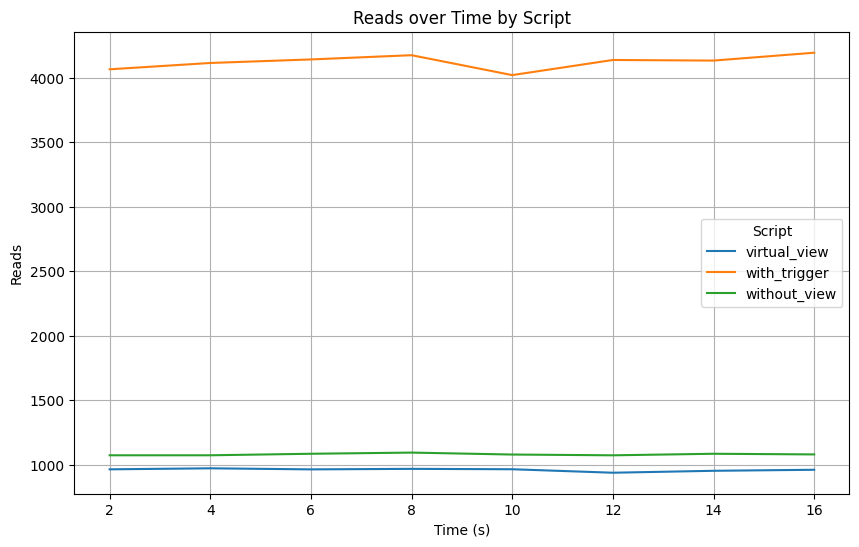
\includegraphics[width=\textwidth]{PNGs/Script/Views/view-comparison/Reads}
    \end{subfigure}
    \hfill
    \begin{subfigure}[t]{0.48\textwidth}
        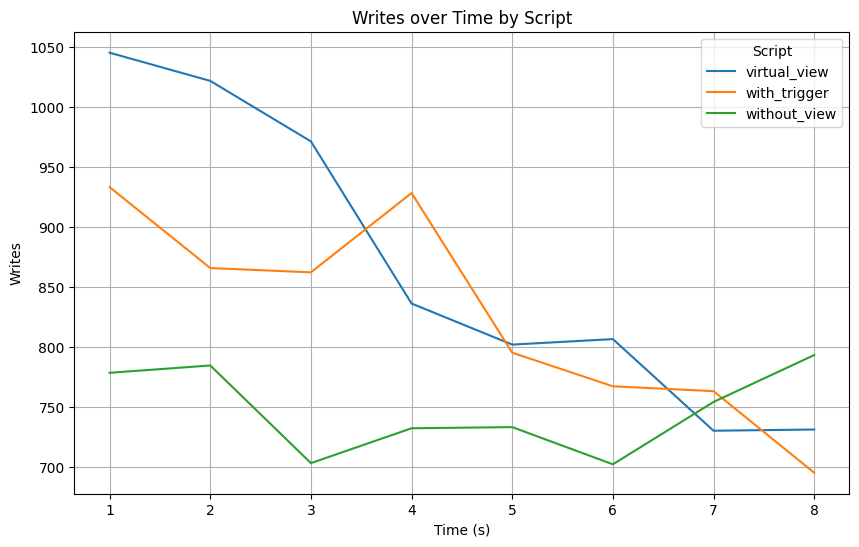
\includegraphics[width=\textwidth]{PNGs/Script/Views/view-comparison/Writes}
    \end{subfigure}
    \vspace{-5pt}
    \caption[Views: Keine View, virtuelle View und Ansatz mit Triggern]{Vergleich zwischen keiner View, der virtuellen und Triggeransatz in MySQL}
    \label{fig:view-comparison-comp-metric}
\end{figure}
\vspace{-15pt}

Bei den Ergebnissen fällt auf, dass die Unterschiede zwischen der virtuellen Sicht und den direkten SQL-Befehlen (\texttt{without\_view}) nur minimal sind.
Dennoch weist \texttt{with\_view} eine leicht schlechtere Performance auf, sowohl bei Lese- als auch bei Schreiboperationen (\ref{fig:view-comparison-comp-metric}).
Einen klaren Performancevorteil kann man beim Trigger-Ansatz erkennen, da die Lesewerte etwa um den Faktor 3 höher sind.
Das liegt daran, dass direkt die Tabelle mit den aggregierten Werten abgefragt wird, wodurch weniger Rechenaufwand erforderlich ist.
Anders hingegen sieht es bei der Schreibperformance aus, da die Trigger ausgelöst werden und zusätzliche Aktualisierungen an der Tabelle \texttt{KUNDEN\_MAT\_OVERVIEW} durchführt werden müssen.
Dadurch sehen wie einen deutlichen Unterschied zu den anderen beiden Ansätzen, da die Werte bei den Schreibvorgängen etwa 15--20\% langsamer sind.

Im letzten Benchmark sollen unterschiedliche Implementierungen von materialisierten Sichten getestet werden.
Dazu wird der Ansatz mit Triggern in MySQL mit der nativen Implementierung in PostgreSQL verglichen.
Die materialisierte Sicht in Postgres kann mithilfe des Befehls aus~\ref{lst:create_mat_view} direkt erstellt werden.
Da Postgres die inkrementeller Auffrischung nicht unterstützt, muss die materialisierte Sicht nach den \texttt{INSERT} und \texttt{DELETE}-Befehlen auf der Kundentabelle immer vollständig aktualisiert werden.
Da der Einfluss auf die Performance des Befehls~\ref{lst:refresh-materialized-view} untersucht werden soll, wird dieser einmal nach der Einfügung jeder Zeile in die Kundentabelle und einmal, nachdem alle Datensätze eingefügt wurden, ausgeführt.

Um die Performanceunterschiede zwischen PostgreSQL und MySQL zu ermitteln, wird der Trigger-Ansatz auch in PostgreSQL implementiert.
Die Implementierungen für die Insert- und Select-Befehle sind bei beiden DBMS identisch, bei der Erstellung der Tabellen und Trigger gibt es aber Unterschiede.
Zum einen unterscheiden sich die Mechanismen zur automatischen Generierung von Primärschlüsseln, da PostgreSQL \texttt{SERIAL} und MySQL \texttt{AUTO\_INCREMENT} verwendet.
Zum anderen kann in MySQL die Logik eines Triggers direkt in der \texttt{CREATE TRIGGER}-Anweisung definiert werden, während in PostgreSQL ein Trigger eine separate Funktion aufrufen muss, die die Logik enthält und mit \texttt{RETURNS TRIGGER} definiert ist.
Auch die Deklarierung der Variablen unterscheidet sich, da in PostgreSQL mehrere Variablen in einem \texttt{DECLARE}-Block und in MySQL jede Variable einzeln im \texttt{BEGIN...END}-Block deklariert werden muss.

\vspace{-5pt}
\begin{figure}[H]
    \centering
    \begin{subfigure}[t]{0.48\textwidth}
        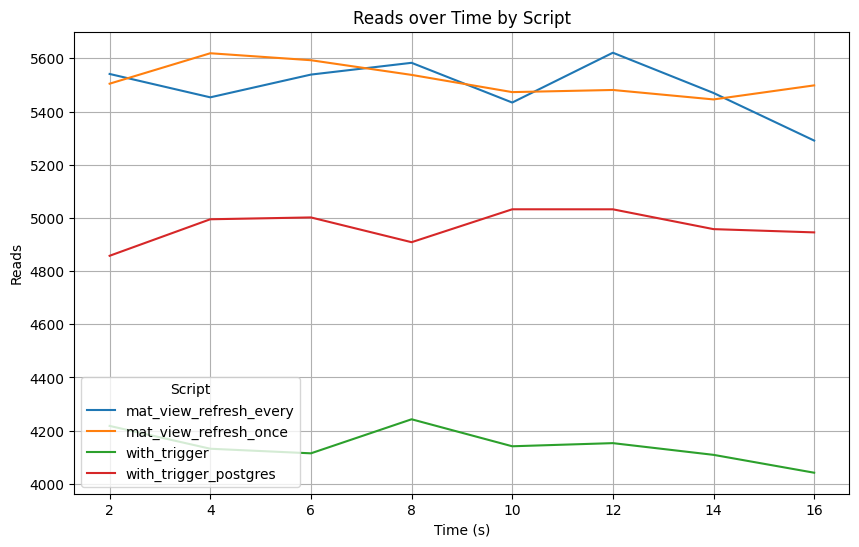
\includegraphics[width=\textwidth]{PNGs/Script/Views/mat-view-comparison//Reads}
    \end{subfigure}
    \hfill
    \begin{subfigure}[t]{0.48\textwidth}
        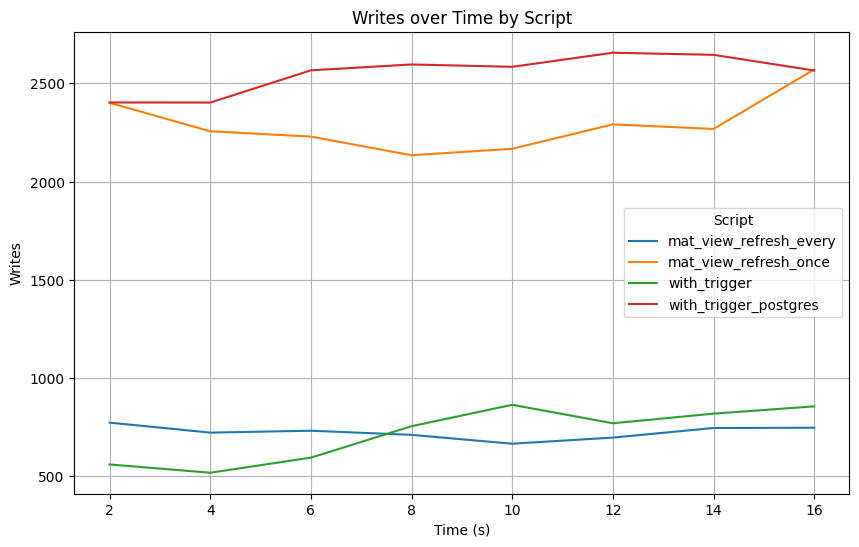
\includegraphics[width=\textwidth]{PNGs/Script/Views/mat-view-comparison/Writes}
    \end{subfigure}
    \vspace{-5pt}
    \caption[Views: Beide Triggeransätze sowie materialisierte Sicht]{Vergleich zwischen Triggeransatz in MySQL und Postgres, sowie zwei nativen Implementierungen in Postgres }
    \label{fig:mat-view-comparison-comp-metric}
\end{figure}
\vspace{-15pt}

Bei der Grafik~\ref{fig:mat-view-comparison-comp-metric} wird zuallererst ein sehr deutlicher Performanceunterschied beim Ansatz mit den Triggern zwischen PostgreSQL und MySQL sichtbar.
Begründet werden kann dieser Unterschied mit den verschiedenen Vorteilen des jeweiligen DBMS und dessen Umgebung.
Beide Systeme wurden mit dem gleichen Ansatz gebenchmarkt, um die Implementierung der nativen materialisierten Sicht, die nur in PostgreSQL möglich ist, besser vergleichen zu können.
Denn die Ergebnisse der nativen Implementierung sind in Bezug auf die Abfragegeschwindigkeit tatsächlich am performantesten und die Anzahl an Aktualisierungen (\ref{lst:refresh-materialized-view}) hat dabei keinen Einfluss.
Anders hingegen sieht es bei der Einfüge-Geschwindigkeit aus, da dort die Implementierung, die nach jedem Insert-Befehl aktualisiert nicht am schnellsten, sondern am langsamsten ist.
Der Vergleich zwischen den Datenbankmanagementsystemen fällt wieder schwer, da die Unterschiede zwischen \texttt{with\_trigger} und \texttt{with\_trigger\_postgres} sehr groß sind (etwa um Faktor 2--3).
Damit wird noch einmal deutlich wie stark die Einfügedauer bei den materialisierten Sichten von der Anzahl an Refreshs abhängig ist, da \texttt{mat\_view\_refresh\_every} unterhalb der Performance von \texttt{with\_trigger} liegt.
In vorliegenden Beispiel ist die einmalige Aktualisierung der Sicht besser als das Verwenden der Trigger in Postgres.

Es lässt sich also zusammenfassen, dass virtuelle Sichten wenig Auswirkungen auf die Performance haben.
Dies ist im eigentlichen Sinne aber auch nicht der Absicht der virtuellen Sicht, denn sie ist besser geeignet, um beispielsweise die Organisation der Rechte für unterschiedliche Nutzer der Datenbank zu gewährleisten.
Wenn man hingegen beispielweise in OLTP-Systemen die Notwendigkeit hat, dass man aggregierte Daten häufig zu der Analyse von bestimmten Daten benötigt, dann sind materialisierte Sichten nützlich.
Man sollte allerdings vor allem die Performanceauswirkungen von diesen Sichten nicht unterschätzen und sich gut überlegen, wie häufig und zu welcher Zeit die Daten aktualisiert werden müssen.
%! Author = danielmendes
%! Date = 13.02.25

\chapter{Replikation}\label{ch:replikation}
In diesem Kapitel befassen wir uns mit dem Thema Replikation.
Replikation ist die Grundlage für den Aufbau großer, leistungsstarker Anwendungen auf der Basis von MySQL\@.
Es verfolgt dabei die sogenannten "Scale-Out"-Architektur, bei der mehrere Storage-Knoten parallelisiert arbeiten und nach außen wie ein einziges Gesamtsystem (\cite{scale_out_eigenschaften}).
Dadurch ist die Skalierbarkeit nahezu unbegrenzt durch das einfache Hinzufügen weiterer Speicherknoten und nicht wie bei Scale-Up durch die Systemgrenzen eines einzelnen Geräts limitiert.
Es trägt allerdings auch Nachteile mit sich, zu denen wir u.a.\ auch später in diesem Abschnitt kommen.
In schon in den vorherigen Kapiteln gehen wir zuerst auf die Grundlagen ein, dann betrachten wir die Konfiguration, die die Basis für die Benchmarks bilden und abschließend analysieren wir die Ergebnisse.

\section{Grundlagen}\label{sec:replication-grundlagen}
Replikation ermöglicht die Konfiguration eines oder mehrere Server als Replicas eines anderen Servers, auch Master genannt (\cite[pp. 447--477]{schwartz2012high}).
Neben der Begrifflichkeit Master-Replika, sind auch die Varianten Primary-Secondary, als auch Master-Slave üblich.
Das grundlegende Problem, das die Replikation löst, besteht darin, die Daten eines Servers mit denen eines anderen synchron zu halten.
Es können sich mehrere Replicas mit einem einzigen Master verbinden und mit diesem synchron bleiben.
Master und Replicas können in vielen verschiedenen Konfigurationen angeordnet werden.
Neben der klassischen Master-Replica-Variante können Replicas selbst als Master für weitere Replicas dienen.
Zudem ist auch eine Master-Master-Kombination möglich.
Das Prinzip der Replikation ist nicht nur für eine höhere Effizienz vorteilhaft, sondern auch für hohe Verfügbarkeit, Skalierbarkeit und Datenanalysen im Data Warehousing, aber sollte keine richtigen Backups ersetzten.
Effizienzvorteile gibt es insbesondere durch die Lastverteilung, die Leseanfragen auf mehrere Server verteilt werden, was besonders für leselastige Anwendungen vorteilhaft ist.
Außerdem kann man das Ganze mit Methoden wie Round-Robin-DNS oder Loadbalancer optimieren.

Im folgenden Abschnitt erklären wir die Funktionsweise der Replikation und betrachten dabei den einfachen Fall mit einem Master und einem oder mehreren Replicas.
Unmittelbar bevor jede Transaktion, die Daten aktualisiert, auf dem Master abgeschlossen wird, zeichnet der Master die Änderungen in seinem Binärlog (engl.\ binary log) auf.
MySQL schreibt Transaktionen seriell im Binary-Log und teilt nach dem Schreiben der Ereignisse den Storage Engines mit, die Transaktionen zu committen.
Zu diesen Änderungen können beispielsweise neu deklarierte Tabellen oder Trigger sowie Einfügeoperationen in bestehende Tabellen gehören.
Im nächsten Schritt muss die Replica die Veränderungen auf dem Master mitbekommen.
Dazu wird ein Worker-Thread gestartet, der als I/O-Slave-Thread bezeichnet wird, und eine Client-Verbindung zum Master geöffnet.
Anschließend wird ein spezieller Prozess (binlog dump process) gestartet, der die Ereignisse aus dem Binary-Log des Masters liest.
Nach dem Verarbeiten schreibt der Thread die Werte auf seine eigene Festplatte, in das sogenannte Relay-Log.
Wenn er alle Ereignisse auf dem Log verarbeitet hat, geht er in einen passiven Zustand und wartet auf Aktualisierungen.
Den letzten Teil des Prozesses übernimmt der SQL-Slave-Thread.
Er liest und spielt Ereignisse aus dem Relay-Log ab und aktualisiert so die Daten des Replicas, sodass sie mit denen des Masters übereinstimmen.
Wenn dieser Thread eine etwa gleich schnelle Verarbeitung wie der I/O-Thread, dann bleibt das Relay-Log normalerweise im Cache des Betriebssystems, sodass Relay-Logs nur sehr geringe Overhead-Kosten haben.
Die Ereignisse, die der SQL-Thread ausführt, können optional zusätzlich in das eigene Binary-Log des Replicas geschrieben werden.

\begin{figure}[!ht]
  \centering
  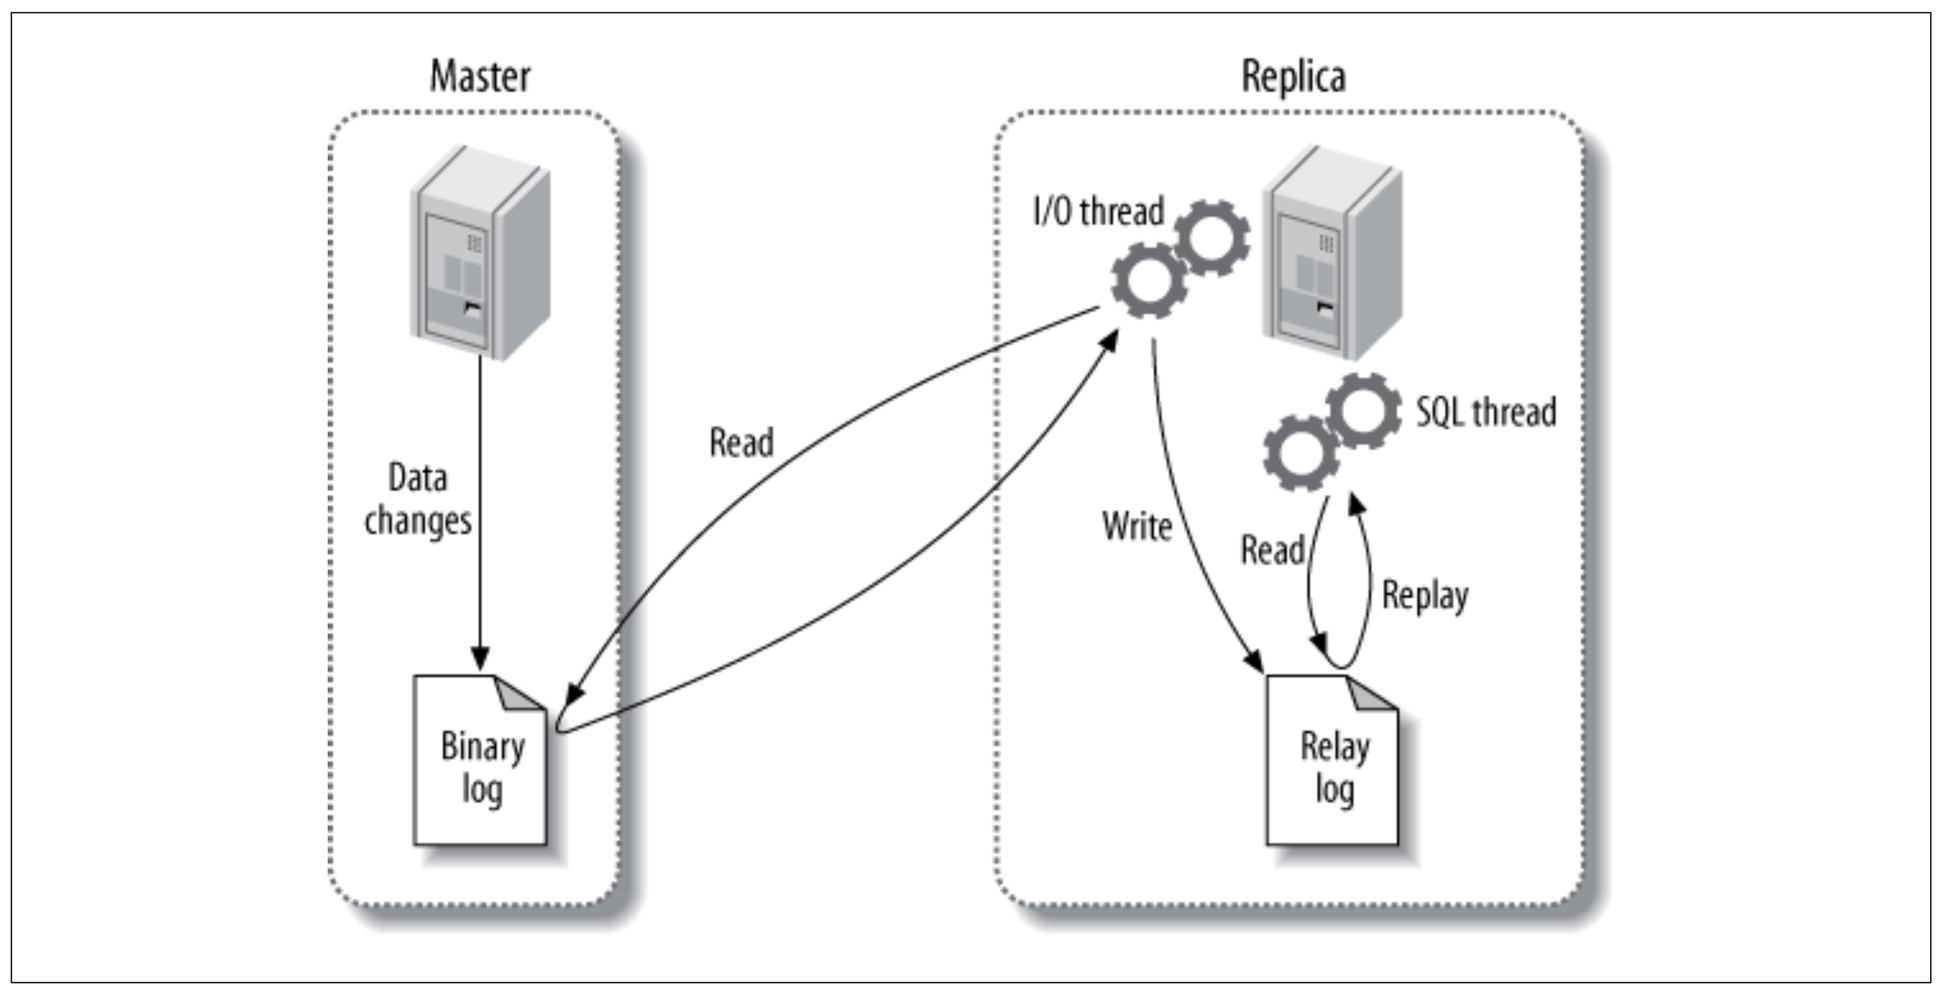
\includegraphics[width=.8\textwidth]{PNGs/Textbook/Master_Replica}
  \caption[Master - Replica - Grafik]{Darstellung der unterschiedlichen Threads}
  \label{fig:master-replica}
\end{figure}

Die Abbildung~\ref{fig:master-replica} zeigt nur die beiden Replikation-Threads, die auf dem Replica laufen.
Zusätzlich gibt es jedoch einen weiteren Thread auf dem Master, da die vom Replica zum Master geöffnete Verbindung einen Thread auf dem Master startet, ähnlich wie jede andere Verbindung zu einem MySQL-Server.

Diese Replikationsarchitektur entkoppelt die Prozesse des Abrufens und Abspielens von Ereignissen auf dem Replica.
Dadurch können die beiden Threads asynchron arbeiten, sodass der I/O-Thread unabhängig vom SQL-Thread agieren kann.
Dies hat jedoch zur Folge, dass Änderungen, die parallel in verschiedenen Threads auf dem Master ausgeführt werden könnten, auf dem Replica nicht parallelisiert werden können, da sie in einem einzelnen Thread ausgeführt werden.
Generell gibt es keine Garantie für die Latenz auf der Replica und große Abfragen können dazu führen, dass die Replica Sekunden, Minuten oder sogar Stunden hinter dem Master zurückbleibt.
Der Flaschenhals (engl.\ bottleneck) des gesamten Systems stellt die Anzahl der Schreibvorgänge dar, die der langsamste Thread ausführen kann.

Die Replikation fügt dem Master nur wenig Overhead hinzu.
Das binäre Logging, das für ordnungsgemäße Backups und Point-in-Time-Recovery erforderlich ist, kann jedoch einen erheblichen Overhead verursachen.
Abgesehen davon verursacht jede angeschlossene Replica nur geringe Last (hauptsächlich Netzwerk-I/O) auf dem Master.
Das Anbinden vieler Replicas an einen Master führt einfach dazu, dass die Schreibvorgänge mehrfach ausgeführt werden, jeweils einmal auf jeder Replika.
Trotzdem sollte man nicht zu leichtfertig mit der Anzahl an Replicas übertrieben, da dadurch im Wesentlichen viele Daten unnötig dupliziert werden.
Bei sehr hoher Arbeitslast (z.B.\ 5.000 Transaktionen pro Sekunde) und vielen Replicas kann der Overhead durch das Aktivieren aller Replica-Threads jedoch erheblich werden.
Replikation eignet sich gut zum Skalieren von Lesevorgängen.

Die Replikation von MySQL ist größtenteils abwärtskompatibel, d.h.\ dass ein neuerer Server in der Regel problemlos als Replika eines älteren Servers fungieren kann.
Andersherum kann es aber zu Fehler kommen, da möglicherweise neue Funktionen oder die SQL-Syntax des neueren Servers nicht verstanden werden kann.
In unserem Beispiel verwenden wir ohnehin nur eine MySQL-Version (siehe~\ref{sec:replication-durchfuhrung}).

Es gibt zwei verschiedene Arten der Replikation, die von MySQL unterstützt werden: die anweisungsbasierte (engl.\ statement-based) und die zeilenbasierte (engl.\ row-based) Replikation.
Die anweisungsbasierte Replikation wird seit MySQL 5.0 und älter unterstützt und funktioniert, indem die Abfrage, die die Daten auf dem Master geändert hat, protokolliert wird.
Wenn eine Replica das Ereignis aus dem Relay-Log liest und ausführt, wird die tatsächliche SQL-Abfrage erneut ausgeführt, die der Master ausgeführt hat.
Der offensichtlichste Vorteil davon ist, dass sie relativ einfach zu implementieren und das Protokollieren und Wiederholen von den Anweisungen sollte die Replica logischerweise mit dem Master synchron halten.
Außerdem sind die Binary-Log-Ereignisse in der Regel recht kompakt sind und verbrauchen nicht viel Bandbreite.
In der Praxis gibt es jedoch Änderungen auf dem Master, die von Faktoren abhängen, die über den reinen Abfragetext hinausgehen.
Beispielsweise werden Anweisungen zu leicht oder sogar deutlich unterschiedlichen Zeiten auf dem Master und dem Replica ausgeführt.
Deshalb muss der Binary Log nicht nur der Abfragetext enthalten, sondern auch Metadaten wie den aktuellen Zeitstempel.
Es gibt einige Anweisungen, die MySQL nicht korrekt replizieren kann, z.B.\ Abfragen, die die Funktion CURRENT\_USER() verwenden und gespeicherte Routinen und Trigger sind ebenfalls problematisch bei dieser Art der Replikation.

Die zeilenbasierte Replikation speichert die tatsächlichen Datenänderungen im Binary-Log.
Ein großer Vorteil, der daraus folgt, ist es, dass MySQL jede Anweisung korrekt replizieren kann.
Zudem können einige Änderungen mithilfe der zeilenbasierte Replikation effizienter sein, da die Replica die Abfragen, die die Zeilen auf dem Master geändert haben, nicht erneut ausführen muss.
Dies ist beispielsweise der Fall, wenn eine Abfrage viele Zeilen in der Quelltabelle scannt, jedoch nur zu drei Zeilen in der Zieltabelle ausführt.
Bei der anweisungsbasierten Replikation müsste eine Replica die Anweisung erneut ausführen, nur um ein paar Zeilen zu erstellen und bei der Zeilenbasierte ist dies effizient und trivial.
Andererseits ist das folgende Ereignis deutlich günstiger mit statement-basierter Replikation zu replizieren:

\vspace{-5pt}
\begin{lstlisting}[language=SQL,caption=Update-Befehl auf dem Master,label={lst:repl_update_command}]
UPDATE master_table SET col1 = 0;
\end{lstlisting}
\vspace{-5pt}

Die Verwendung von zeilenbasierte Replikation für diese Abfrage wäre sehr teuer, da jede Zeile geändert wird und damit auch ins Binary-Log geschrieben müsste, was das Binary-Log-Ereignis extrem groß machen würde.
Dies würde sowohl beim Protokollieren als auch bei der Replikation zu einer höheren Last auf dem Master führen.
Die Durchführung einer Point-in-Time-Wiederherstellung ist mit einem Binary-Log im row-based Format schwieriger, aber nicht unmöglich.

Insgesamt ist die anweisungsbasierte Replikation besser geeignet, wenn das Schema auf dem Master und dem Replikat unterschiedlich ist, und kann in Szenarien eingesetzt werden, in denen Tabellen unterschiedliche, aber kompatible Datentypen, verschiedene Spaltenreihenfolgen usw.\ aufweisen.
Außerdem vereinfacht es das Durchführen von Schema-Änderungen auf einem Replica, das später als Master verwendet werden soll, um möglicherweise die Ausfallzeit zu reduzieren.
Die zeilenbasierte Replikation kann jedoch einige Operationen bei Schema-Änderungen auf einem Replica nicht handhaben.
Dafür aber funktioniert sie zuverlässig mit allen SQL-Konstrukten und es gibt weniger Fälle, in denen es zu Problemen kommt.
Auch stoppt sie bei Fehlern, z.B.\ wenn eine erwartete Zeile auf dem Replikat fehlt, was jedoch auch als Vorteil betrachtet werden kann, da es auf Inkonsistenzen hinweist.
Bei der anweisungsbasierte Replikation führt ein Update auf dem Master zu keinem Fehler, wenn die Zeile auf dem Replica fehlt.
Die zeilenbasierte Replikation erkennt diesen Fehler und stoppt die Replikation, was eine sofortige Überprüfung ermöglicht.
Bei der anweisungsbasierten Replikation erfolgen alle Änderungen über einen bekannten Mechanismus (SQL-Anweisungen), was die Fehlersuche und das Verständnis von Problemen erleichtert, aber es erfordert auch mehr Sperren (Locks).
Genau andersherum sieht es bei der Zeilenbasierte aus, da dort Nachvollziehbarkeit von Änderungen ohne die Speicherung der ursprünglichen SQL-Anweisung erschwert wird, aber dafür gibt es reduziertes Locking.
Die zeilenbasierte Replikation hat auch Vorteile bei der Datenwiederherstellung, da in einigen Fällen auch alte Daten gespeichert werden, was die Wiederherstellung erleichtert.
Auch benötigt sie oft weniger CPU-intensiv, da keine komplexe SQL-Parsing- und Ausführungslogik erforderlich ist und es gibt auch Probleme bei der mehrstufigen Replikation.
Denn wenn eine Anweisung mit @@binlog\_format = STATEMENT auf dem Master ausgeführt wird, dann wird sie dort als Statement protokolliert.
Die nachgelagerte Replicas (Second-Level-Replicas) können diese jedoch als row-basiert weiterleiten, was zu Inkonsistenzen bei der Protokollierung führt.

Da kein Format in jeder Situation perfekt ist, kann MySQL dynamisch zwischen statement-basierter und row-basierter Replikation wechseln
Standardmäßig wird die statement-basierte Replikation verwendet, aber wenn MySQL ein Ereignis erkennt, das nicht korrekt als Statement repliziert werden kann, wechselt es automatisch zur row-basierten Replikation
Sie können das Format auch manuell steuern, indem Sie die Session-Variable binlog\_format setzen

\section{Durchführung}\label{sec:replication-durchfuhrung}

Für die Durchführung nutzen wir wieder die Kundentabelle (\ref{lst:create_table_kunde}) und die Bestelltabelle (\ref{lst:create_table_bestellung}), die wir schon aus dem Beispiel aus Kapitel~\ref{sec:projektaufbau-mit-beispiel} kennen.
Die einzige Anpassung, die wir vornehmen müssen, sind die unterschiedlichen Werte \texttt{STATEMENT}, \texttt{ROW} und \texttt{MIXED}, die die Variable \texttt{binlog\_format} annehmen kann.

\vspace{-5pt}
\begin{lstlisting}[language=SQL,caption=Unterschiedliche Formatimplementationen,label={lst:repl_change_format}]
SET SESSION binlog_format = 'STATEMENT'
SET SESSION binlog_format = 'ROW'
SET SESSION binlog_format = 'MIXED'
\end{lstlisting}
\vspace{-5pt}

Damit können wir die Performanceunterschiede zwischen den einzelnen Arten, insbesondere für die Einfügeoperationen, vergleichen.
Wie wir sehen, sind die Veränderungen an den Lua-Skripten damit minimal, aber der eigentliche Aufwand entsteht bei der Einrichtung der Replikation auf dem lokalen Rechner und in einem Workflow.

Für die Benchmarks betrachten wir das einfachste Szenario der Replikation, bestehend aus einem Master und einer beliebigen Anzahl an Replicas.
Zunächst müssen wir dazu den Master und die Replikationsknoten dazu konfigurieren und anschließend dem Replikat anweisen, sich mit dem Master zu verbinden und von ihm zu replizieren.
MySQL hat einige spezielle Privilegien, die es den Replikationsprozessen erst ermöglichen, zu laufen.
Dazu muss ein Benutzer auf dem Master erstellt werden und diesem die richtigen Privilegien zugewiesen werden, damit der I/O-Thread sich als dieser Benutzer verbinden und das Binary-Log des Masters lesen kann.

\vspace{-5pt}
\begin{lstlisting}[language=SQL,caption=Nutzererstellung und Rechtevergabe,label={lst:repl_privileges}]
GRANT REPLICATION SLAVE, REPLICATION CLIENT ON .
\end{lstlisting}
\vspace{-5pt}

Wir erstellen diesen Nutzer sowohl auf dem Master als auch auf dem Replica.
Der Nutzer, der zur Überwachung und Verwaltung der Replikation verwendet wird, benötigt das \texttt{REPLICATION CLIENT} Privileg und daher ist es einfacher, denselben Benutzer für beide Zwecke zu verwenden.
Der nächste Schritt besteht darin, einige Einstellungen auf dem Master zu aktivieren.
Zum einen müssen die Binärprotokollierung aktiviert und eine Server-ID angegeben werden.
Wenn die Binärprotokollierung im Konfigurationsfile des Masters nicht bereits angegeben wurde, müssen Sie MySQL neu starten.
Zum anderen muss explizit eine einzigartige Server-ID angegeben werden.
Um zu überprüfen, ob die Binary-Logdatei auf dem Master erstellt wurde, kann man folgenden Befehl ausführen:

\vspace{-5pt}
\begin{lstlisting}[language=SQL,caption=Anzeige der Konfiguration,label={lst:repl_master_config}]
SHOW BINARY LOG STATUS; --MySQL ≥8.0.23
SHOW MASTER STATUS; --MySQL <8.0.23
\end{lstlisting}
\vspace{-5pt}

Die wichtigste Einstellung für das Binär-Logging auf dem Master ist sync\_binlog: sync\_binlog=1.
Diese Option sorgt dafür, dass MySQL den Inhalt des Binary-Logs, nicht dem Relay-Log, bei jedem Transaktions-Commit auf die Festplatte synchronisiert und damit kommt es zu keinen verlorenen Log-Ereignissen im Falle eines Absturzes.
Wenn diese Option deaktiviert ist, dann hat der Server etwas weniger Arbeitsaufwand, aber Binary-Log-Einträge könnten nach einem Serverabsturz beschädigt oder verloren sein.
Auf einem Replikat, das nicht als Master fungieren muss, erzeugt diese Option unnötigen Overhead.
Außerdem wird es empfohlen einen Basisnamen für das Binary-Log explizit anzugeben, um einheitliche Binary-Log-Namen auf allen Servern zu erstellen und Änderungen der Binary-Log-Namen zu vermeiden, falls sich der Hostname des Servers ändert.
Dazu muss ein Argument für die \texttt{log\_bin}-Option angegeben werden.

Auf einem Replikat ist nur der Parameter \texttt{server\_id} erforderlich, wir haben zudem aber noch zwei andere optionale Konfigurationsparameter, die wir hinzufügen können.
Zum einen den optionalen Konfigurationsparameter \texttt{relay\_log}, der den Speicherort und den Namen des Relay-Logs angibt, sie passend dazu die Option \texttt{log\_bin} für den Master.
Zum anderen \texttt{log\_slave\_updates}, um das Replikat die replizierten Ereignisse in sein eigenes Binary-Log zu schreiben.
Die Option skip\_slave\_start verhindert, dass das Replikat nach einem Absturz automatisch startet und es gibt dadurch die Möglichkeit, den Server bei Problemen zu reparieren.
Die Option read\_only verhindert, dass die meisten Benutzer nicht-temporäre Tabellen ändern.
Ausnahmen sind der Replikation-SQL-Thread und Threads mit dem SUPER-Privileg.
Daher sollte es auch vermieden werden, normalen Benutzerkonten das SUPER-Privileg zu geben.
Die letztere Option verursacht zusätzlichen Aufwand für die Replikate, aber wir haben gute Gründe, diese optionalen Einstellungen auf jedem Replikat hinzuzufügen.
Wenn ein Replikat stark hinter dem Master zurückliegt, kann der Slave-I/O-Thread viele Relay-Logs schreiben.
Der Replikation-SQL-Thread entfernt diese, sobald er mit deren Verarbeitung fertig ist (dies kann mit der Option relay\_log\_purge geändert werden).
Wenn das Replikat stark im Rückstand ist, könnte der I/O-Thread tatsächlich den Speicherplatz der Festplatte füllen.

Ein Replikat kann nach einem Absturz leicht beschädigt werden, da die Relay-Logs und die master.info-Datei nicht absturzsicher sind

Der nächste Schritt besteht darin, dem Replikat zu sagen, wie es sich mit dem Master verbinden kann und wie dessen Binary-Logs abspielen wird.

\vspace{-5pt}
\begin{lstlisting}[language=SQL,caption=Verbindung der Replica zum Master,label={lst:repl_con_replica_master}]
CHANGE MASTER TO
  MASTER_HOST='YOUR_HOST_NAME',
  MASTER_USER='YOUR_USER',
  MASTER_PASSWORD='YOUR_PASSWORD',
  MASTER_LOG_FILE='mysql-bin.000001',
  MASTER_LOG_POS=0;
\end{lstlisting}
\vspace{-5pt}

Die Spalten \texttt{MASTER\_LOG\_FILE} und \texttt{MASTER\_LOG\_POS} müssen mit dem Ergebnis von dem Befehl aus~\ref{lst:repl_master_config} übereinstimmen.
Um die eigentliche Replikation zu starten, muss man den folgenden Befehl ausführen:

\vspace{-5pt}
\begin{lstlisting}[language=SQL,caption=Starten der Replikation,label={lst:repl_replica_start}]
START SLAVE;
\end{lstlisting}
\vspace{-5pt}

Mit dem folgenden Befehl kann man überprüfen, ob das Ganze erfolgreich war oder nicht.

\vspace{-5pt}
\begin{lstlisting}[language=SQL,caption=Status der Replica,label={lst:repl_replica_status}]
SHOW PROCESSLIST\G;
\end{lstlisting}
\vspace{-5pt}

Die Spalten \texttt{Slave\_IO\_State}, \texttt{Slave\_IO\_Running} und \texttt{Slave\_SQL\_Running} zeigen an, dass die Replikationsprozesse nicht laufen oder nicht.
Wenn \texttt{Seconds\_Behind\_Master} nicht mehr NULL ist, dann bedeutet das, dass der I/O-Thread auf ein Ereignis vom Master wartet, weil er schon alle Binary-Logs abgerufen hat.
Wenn man Änderungen an dem Master vornimmt, dann sollte man beobachten, dass die verschiedenen Datei- und Positionswerte auf dem Replikat inkrementiert werden und auch die Änderungen in den Datenbanken sollten auf dem Replikat sichtbar sein.
Außerdem sollten zwei Threads auf dem Replikat aktiv sein, die immer unter dem Benutzerkonto "system user" laufen.

Bei den vorherigen Setup-Anweisungen sind wir von einer frischen Installation ausgegangen.
Es gibt aber auch andere Möglichkeiten, um ein Replikat von einem anderen Server zu initialisieren und zwar das Kopieren von Daten von einem Master, das Klonen eines Replikats von einem anderen Replikat oder das Starten eines Replikats von einem aktuellen Backup.
Um ein Replikat mit einem Master zu synchronisieren, sind drei Elemente erforderlich: eine Momentaufnahme der Master-Daten zu einem bestimmten Zeitpunkt, die Log-Datei des Masters mit dem entsprechenden Byte-Offset (ermittelbar durch den Befehl~\ref{lst:repl_master_config}) sowie die Binary-Logs des Masters ab diesem Zeitpunkt.
Eine kalte Kopie erfordert das Herunterfahren des Masters, um dessen Dateien zu kopieren, bevor er mit einem neuen Binary-Log neu gestartet wird, was jedoch zu Ausfallzeiten führt.
Bei einer warmen Kopie können die Dateien übertragen werden, während der Server weiterhin läuft.

\section{Analyse}\label{sec:replication-analyse}

Im vorherigen Abschnitt wurde erklärt, wie man die Master und vor allem die Replicas korrekt konfiguriert und den Prozess der Replikation startet.
Es wurde auch erklärt, wie wir das Binlog-Format verändern können und dass wir das Lua-Skript mit den Kunden- und Bestelltabelle verwenden.
Als Nächstes analysieren wir zwei unterschiedliche Situationen.

Im ersten Vergleich wollen wir die Performanceunterschiede zwischen den Master-Replica-Ansatz und dem Ansatz mit einem MySQL-Server feststellen.
Beim Master-Replica-Ansatz verwenden wir mit \texttt{ROW} immer den Default-Wert des Binlog-Formats.
Damit keine Fehler auftreten, müssen wir die beiden Ansätze miteinander kompatibel machen.
Das Problem dabei ist, dass nicht beide den Standardport von MySQL (3306) gleichzeitig nutzen dürfen.
Deshalb starten wir den Master mit der Port 3307 und die Replicas inkrementieren diesen Wert jeweils um 1.
Entsprechend hat die 3.\ Replica den Port 3310.
Die Anzahl an Replicas können wir in der \texttt{envs.json}-Datei mithilfe der Variablen \texttt{REPLICAS\_COUNT} festlegen.
Dementsprechend muss es mit der Anzahl lokal oder innerhalb eines Workflowjobs gestarteten und konfigurierten Replicas übereinstimmen.
Wichtig ist noch zu erwähnen, dass beim Master-Replica logischerweise die Insert-Befehle nur auf dem Master also Port 3307 ausgeführt werden.
Die Select-Befehle werden sowohl auf dem Master als auch auf den Replicas ausgeführt.

\vspace{-8pt}
\begin{figure}[H]
  \centering
  \begin{subfigure}[t]{0.48\textwidth}
    \centering
    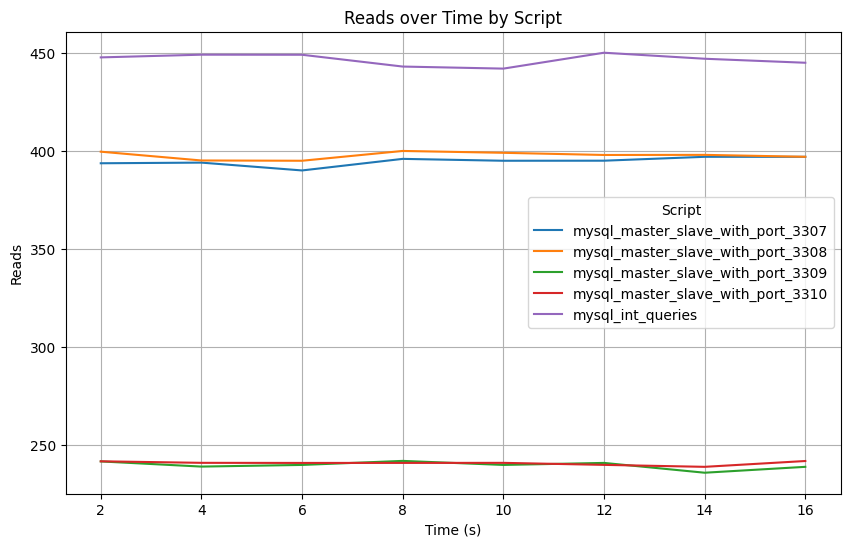
\includegraphics[width=\textwidth]{PNGs/Script/Replication/replication-vs-no/Reads}
    \label{replication-vs-no-reads}
  \end{subfigure}
  \hfill
  \begin{subfigure}[t]{0.48\textwidth}
    \centering
    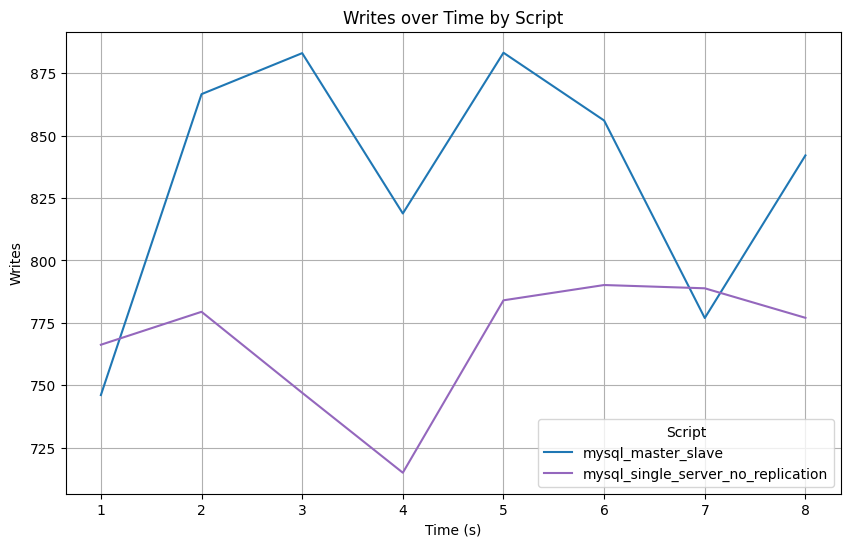
\includegraphics[width=\textwidth]{PNGs/Script/Replication/replication-vs-no/Writes}
    \label{replication-vs-no-writes}
  \end{subfigure}
  \vspace{-20pt}
  \caption[Replikation: Metrikvergleich]{Vergleich zwischen dem Master-Replica-Ansatz und einem normalen MySQL-Server }
  \label{fig:replication-vs-no}
\end{figure}
\vspace{-20pt}

Wenn wir die Ergebnisse aus Abbildung~\ref{fig:replication-vs-no} betrachten, dann fällt auf, dass die Version ohne Replikation am schnellsten ist.
Danach folgen die Readabfragen auf dem Master auf Port 3307.
Der Unterschied der beiden liegt bei ~ 15\%.
Nah an dem Ergebnis vom Master ist die erste Replica (3308).
Überraschenderweise folgen danach die anderen beiden Replicas auf den Ports 3309 und 3310.
Die Writegeschwindigkeit ist in beim Fall ohne und mit Replikation auf einem ähnlichen Niveau.

Im zweiten Vergleich benutzen wir ausschließlich den Master-Replica-Ansatz.
Dafür vergleichen wir aber die unterschiedlichen Binlog-Formate, die wir aus~\ref{lst:repl_change_format} kennen.
Um Variationen zu begrenzen, betrachten wir nur eine Replica pro Master.
Das ergibt sechs unterschiedliche Leseergebnisse, da wir pro Format zwei Ports abfragen.
Einmal den Master-Port und einmal den Port der einzigen Replica.
In der Grafik~\ref{fig:replication-format-change} können wir sehen, dass die Unterschiedliche kaum erkennbar sind bei verschiedenen Binlog-Formaten und Ports.
Und auch die Schreibgeschwindigkeiten verhalten sich bei beiden Varianten sehr ähnlich.

\begin{figure}[H]
  \centering
  \begin{subfigure}[t]{0.48\textwidth}
    \centering
    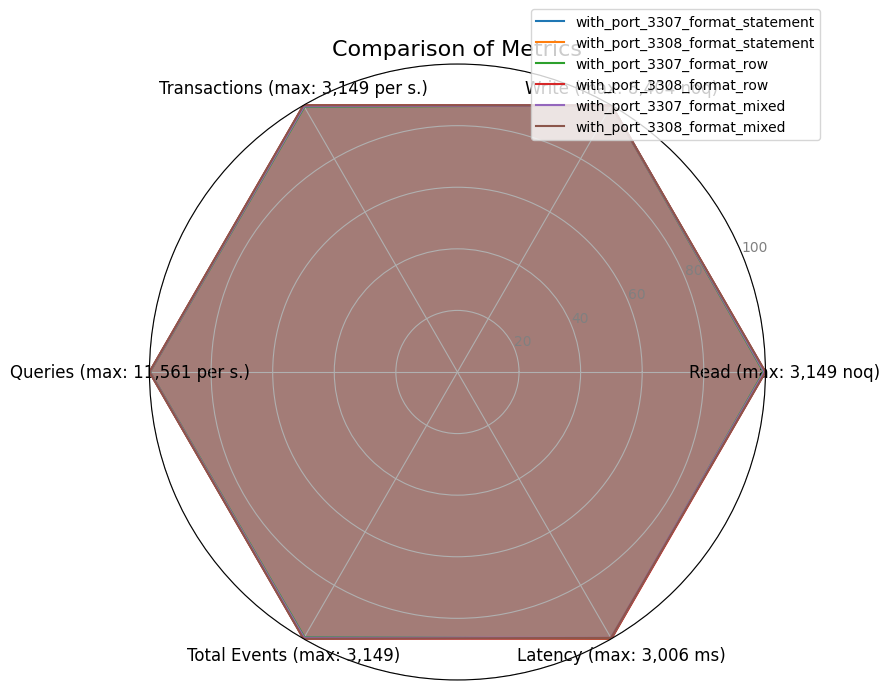
\includegraphics[width=\textwidth]{PNGs/Script/Replication/replication-format-change/statistics}
    \label{replication-format-change-statistics}
  \end{subfigure}
  \hfill
  \begin{subfigure}[t]{0.48\textwidth}
    \centering
    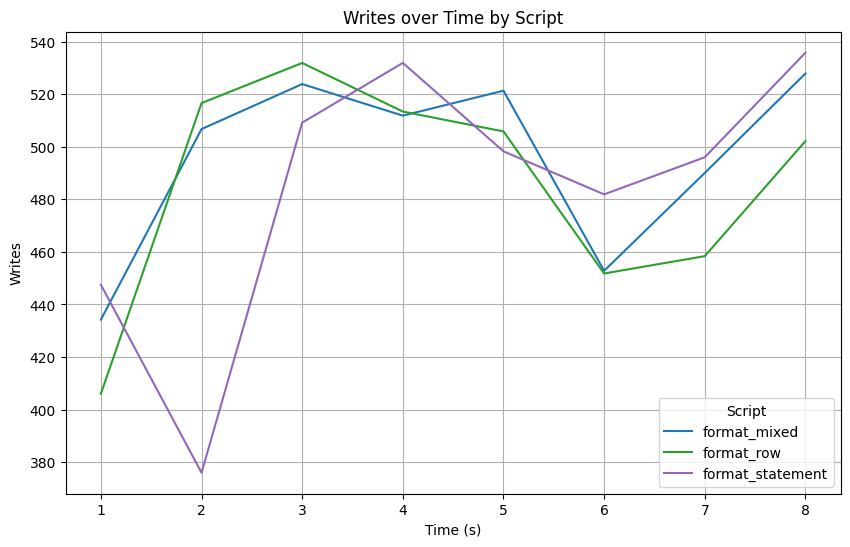
\includegraphics[width=\textwidth]{PNGs/Script/Replication/replication-format-change/Writes}
    \label{replication-format-change-writes}
  \end{subfigure}
  \vspace{-20pt}
  \caption[Replikation: Metrikvergleich]{Vergleich zwischen dem unterschiedlichen Binlog-Typen }
  \label{fig:replication-format-change}
\end{figure}
\vspace{-20pt}

Die Schlussfolgerungen, die wir aus den Messungen gewinnen können, sehen dabei wie folgt aus.
Wir sehen, dass durch Replication, anders als beispielsweise mit Indexen oder Partitionen, keine deutliche Performancevorteile gewonnen werden.
Zum einen könnte sich in einer realen Umgebung anders verhalten, aber zum anderen hat die Replikation andere Vorteile.
Wenn meherere Nutzer auf der Datenbank interagieren und ausschließlich Lesezugriffe benötigen, dann können die Abfragen auf die unterschiedlichen Ports aufgeteilt werden.

TODO: Verteilung auf unterschiedliche Ports durch Sysbench umsetzbar???

%! Author = danielmendes
%! Date = 20.01.25
\chapter{Fazit}\label{ch:fazit}

Die vorliegende Bachelorarbeit ging der Frage nach, wie die Performance einer relationalen Datenbank verbessert werden kann.
Ihr Aufbau orientiert sich am Prozess des Datenentwurfs.
Beim Datenbankentwurf muss man die ermittelten Anforderungen aus den Interviews mit Stakeholdern verwenden, um einen konzeptionellen Entwurf, beispielsweise in Form eines ER-Modells, zu erstellen.
Danach wird aus dem konzeptionellen Entwurf ein Logischer in Form eines Relationenschemas.
Dieses Kapitel dient dazu, eine allgemeine Zusammenfassung der wesentlichen Erkenntnisse zu bieten.

Zuallererst wird der logische Entwurf betrachtet, bei dem neben der Normalisierung der Tabellen auch die Auswahl der korrekten Datentypen eine Rolle spielt.
Das erste Kapitel behandelte dieses Thema im Detail.
Mithilfe der Benchmarks wurde festgestellt, dass der kleinstmögliche Datentyp für eine Spalte deklariert werden sollte.
Dazu muss zunächst festgelegt werden, welcher Bereich an Werten abgebildet werden soll, um darauf basierend den geeigneten Typ auszuwählen.
Dabei ist durchaus von Vorteil, dass der Typ bei einer falschen Einschätzung des Wertebereichs ohne viel Aufwand verändert werden kann.
Beim Betrachten der numerischen Datentypen fiel auf, dass je größer der Wertebereich und damit der Speicherbedarf ist, desto schlechter wird die Leistung.
Deshalb zählen \texttt{DECIMAL} und \texttt{BIGINT} zu den ineffizientesten.
Bei den zeichenkettenbasierten Typen ist die Wahl einfach zu treffen, da in den meisten Fällen der Typ \texttt{VARCHAR} am schnellsten ist.
Nur wenn eine Spalte häufiger aktualisiert als abgefragt wird, kann es sinnvoll sein, den Typ \texttt{CHAR} in Erwägung zu ziehen.
Ein weiterer Leitsatz bei der Wahl der Datenformate ist, eine simplere Datenstruktur zu bevorzugen, was sich im Vergleich zeigte, da \texttt{INT} schneller als \texttt{CHAR} ist.
Zu guter Letzt sollte berücksichtigt werden, dass die Spalten nicht nur aus Performancegründen, sondern auch zur Wahrung der Datenintegrität und -konsistenz an möglichst vielen Stellen als \texttt{NOT NULL} definiert werden sollten.
Nach dem logischen Entwurf einer Datenbank kommt als nächster Schritt die physische Implementierung.
Bei diesem Schritt spielen auch die anderen Aspekte, die betrachtet wurden, wie Indexierung, Sichten, Partitionen oder Replikation, eine Rolle.

Bei der Indexierung wurde gezeigt, wie effektiv sie sein kann, indem der Aufbau und die Funktionsweise der B-Tree- und Hash-Indexe erläutert und getrennt voneinander untersucht wurden.
Der Vergleich beider Varianten hat ergeben, dass der Hash-Index in bestimmten Fällen effektiver ist als der B-Baum-Index.
Auf der anderen Seite kann der B-Baum-Index bei deutlichen mehr Abfragen eingesetzt werden, insbesondere auch bei Bereichsabfragen oder Filtern von Teilen des Indexes.
Im Gegensatz dazu funktioniert der Hash-Index nur bei einem exakten Schlüsselabgleich.
Außerdem ist beim Hash-Index auch die Anzahl an Hashkollisionen relevant für die Performance.
Der größte Nachteil der Verwendung von Indizes ist der höhere Pflegeaufwand, da bei jeder Datenänderung der Index ebenfalls angepasst werden muss.
Wenn Performanceprobleme bei einer Datenbankumgebung auffallen, dann sollte man in den Logs nach Abfragen suchen, die zum einen besonders häufig vorkommen und zum anderen viel Zeit benötigen.
Bei der Analyse kann man möglicherweise eine sinnvolle Nutzung von Indizes identifizieren und diese erstellen.
Nach einigen Tagen oder Wochen bietet es sich an, eine Kontrolle durchzuführen und abhängig vom Ergebnis können einige Indizes entfernt und andere neue hinzugefügt werden.
Ein ähnliches Vorgehen ist auch beim Einsatz von Views nützlich.

Wie bei den Benchmarks für die Sichten festgestellt wurde, wirken sich virtuelle Views nicht auf die Performance aus.
Dafür eignen sich virtuelle Sichten hervorragend für Gewährleistung von Rechtemanagement in einer Organisation, denn sie haben den Vorteil, dass die Daten nicht physisch gespeichert werden und somit keine Redundanzen entstehen.
Materialisierte Sichten hingegen werden auf der Festplatte gesichert und bieten dafür ein erhebliches Performancepotenzial.
Besonders geeignet sind sie in Szenarien, in denen häufig auf aggregierte oder komplexe Abfragen zugegriffen wird, wie zum Beispiel in OLTP-Systemen.
Es ist durchaus sinnvoll, sich bereits beim Datenbankentwurf Gedanken über Sichten zu machen, doch es ist auch möglich, diese, wie bei Indizes, erst im Laufe der Zeit zu ergänzen.
Wie genau die Implementierung von materialisierten Sichten umgesetzt werden kann, hängt vom jeweiligen Datenbankmanagementsystem ab.
Einige DBMS unterstützen materialisierte Sichten, während andere sogar eine inkrementelle Auffrischung ermöglichen.
In MySQL hingegen müssen materialisierte Sichten durch dedizierte Tabellen in Kombination mit Triggern nachgebildet werden.
Bei den Tests ist jedoch deutlich geworden, dass die native Implementierung, z.B.\ in Postgres, einen klaren Performancevorteil gegenüber der Implementierung mit Triggern bietet.
Daher sollte dieser Aspekt bei der Auswahl des DBMS berücksichtigt werden.
In Bezug auf die Schreibperformance muss ebenfalls erwähnt werden, dass die Pflege von materialisierten Sichten die Effizienz negativ beeinflusst.

Bei Partitionen fällt der Mehraufwand geringer aus als bei Indizes oder Sichten, da keine zusätzlichen Datenbankobjekte verwaltet werden müssen.
Stattdessen werden die Datensätze auf mehrere Partitionen verteilt und nicht in einer einzelnen Tabelle gespeichert.
Wenn eine Datenbankoperation ausgeführt wird, muss zunächst die Partition oder die entsprechenden Partitionen ermittelt werden, die die angeforderten Daten enthalten.
Normalerweise ist ein Merkmal, das für die Partitionierung spricht, ein natürliches Trennkriterium wie ein Zeitstempel oder geografische Regionen, da dadurch eine logische Aufteilung der Daten ermöglicht wird.
Abhängig vom Trennkriterium muss man sich für einen der Partitionierungstypen entscheiden: Range, List, Hash oder Key.
Der Vorteil der Partitionierung liegt darin, dass nur die relevanten Partitionen durchsucht werden müssen, anstatt die gesamte Tabelle zu scannen.
Dieser Vorgang wird als Pruning bezeichnet und führt zu einer erheblichen Steigerung der Abfragegeschwindigkeit.
Allerdings gibt es einige Einschränkungen beim Pruning.
Bei der Range-Partitionierung mit einem Zeitstempel können bei einigen Operatoren unerwartete Probleme auftreten.
Ein solches Beispiel stellt der \texttt{YEAR()}-Operator dar, der zwar dasselbe Ergebnis wie eine Bereichsabfrage liefert, jedoch nicht für das Partition-Pruning verwendet werden kann.
In einem solchen Fall müssen alle Partitionen durchsucht werden, was die Abfrage sogar langsamer macht als ohne Partitionierung.
Für die List-Partitionierung hat sich gezeigt, dass der Operator \texttt{IN} am effizientesten ist, gefolgt von \texttt{OR}, während \texttt{UNION} deutlich weniger effizient ist, weshalb von seiner Verwendung abgeraten werden sollte.
Die Hash-Partitionierung trägt zu einer gleichmäßigen Verteilung der Daten bei.
Darüber hinaus wurde festgestellt, dass bei dieser sowie den anderen Typen die Komplexität der Suche innerhalb der Partitionierungsstruktur mit einer steigenden Anzahl von Partitionen zunimmt, was zu einer entsprechenden Verschlechterung der Performance führt.

Zum Schluss wurde der Einfluss der Replikation im Rahmen des Master-Replikat-Ansatzes analysiert.
Anders als bei der Partitionierung werden bei der Replikation vollständige Kopien der gesamten Datenbank auf mehreren Servern erstellt.
Wenn Änderungen am Master vorgenommen werden, werden diese durch verschiedene Threads an die Replikate übertragen.
Dadurch wird die Verfügbarkeit und Ausfallsicherheit erhöht, weshalb Replikation häufig in Verbindung mit Backups eingesetzt wird.
Um die Performance zu testen, wurde die Leistung eines Single-Servers mit der eines Systems aus Master- und Replikaten verglichen.
Dabei wurde festgestellt, dass der Single-Server bei Verwendung eines einzelnen Threads einen Leistungsvorteil hat.
Sobald jedoch mehrere Threads die CPU-Auslastung auf dem Single-Server erhöhen und gleichzeitig die Last auf die Master- und Replikatknoten verteilt wird, zeigt sich der Vorteil der Replikationsverteilung.
In Bezug auf die Verteilung zeigt die Replikation Ähnlichkeiten mit den grundlegenden Konzepten von NoSQL-Datenbanken, die ebenfalls horizontale Skalierung einsetzen, um die Effizienz zu optimieren.
Allerdings treten auch Nachteile beim Einfügen von Daten mit Replikation auf, da das erneute Kopieren der Daten auf die Replikate die Performance negativ beeinflusst.

Zusammenfassend lässt sich festhalten, dass es keine allgemeingültige Lösung für optimale Performance gibt, sondern verschiedene Konzepte, deren Effizienz vom jeweiligen Anwendungsfall abhängt.
Oft führt eine gezielte Kombination mehrerer Techniken zu den besten Ergebnissen.
Ein bewährter Ansatz ist die Verbindung von Partitionierung und Replikation.
Hierbei wird jede Partition auf mehreren Knoten repliziert, wodurch die Datensätze weiterhin einer bestimmten Partition zugeordnet bleiben, gleichzeitig aber redundant gespeichert werden.
Darüber hinaus wirkt sich die Verwendung kleinerer Datentypen positiv auf die Index-Performance aus.
Indizes können effektiv mit Partitionierung oder materialisierten Views kombiniert werden und optimieren in replizierten Systemen die Lesezugriffe auf die Replikate.
Letztlich zeigt sich, dass das Zusammenspiel der verschiedenen Strategien eine nachhaltige Antwort bietet.
% -*- coding: utf-8 -*-

% Ausgabe des Literaturverzeichnisses; ohne weitere Optionen werden nur die
% Bücher und Artikel ausgegeben, die in der Arbeit auch zitiert werden.
\printbibliography

% markiert den Anfang des Anhangs
\appendix

% ein Kapitel, das nicht numeriert, aber trotzdem ins Inhaltsverzeichnis
% aufgenommen wird
\addchap{Anhang}
% TODO (Daniel): update here se-app
Hier beginnt der Anhang.  Siehe die Anmerkungen zur Sinnhaftigkeit eines
Anhangs in Abschnitt%~\ref{sec-app} auf Seite~\pageref{sec-app}.

Der Anhang kann wie das eigentliche Dokument in Kapitel und Abschnitte
unterteilt werden.  Der Befehl \verb|\appendix| sorgt im Wesentlichen nur für
eine andere Nummerierung.

% neue Seite
\clearpage

% keine Seitenzahl
\thispagestyle{empty}

% keine Nummerierung, keine Aufnahme ins Inhaltsverzeichnis
\section*{Eigenständigkeitserklärung}

% Hier müssen Sie natürlich den Titel der Arbeit sowie Ort und Datum ersetzen:
Hiermit versichere ich, dass ich die vorliegende Bachelorarbeit mit dem Titel
\begin{center}
  \textbf{Performance - Optimierung von Datenbanken}
\end{center}
selbstständig und nur mit den angegebenen Hilfsmitteln verfasst habe.  Alle
Passagen, die ich wörtlich aus der Literatur oder aus anderen Quellen wie
z.\,B. Internetseiten übernommen habe, habe ich deutlich als Zitat mit Angabe
der Quelle kenntlich gemacht.

\vspace{2cm}
% TODO (Daniel): update this here
Hamburg, 21.\ Dezember 1940

\end{document}